\documentclass[11pt,a4paper,twoside]{tesis}
% SI NO PENSAS IMPRIMIRLO EN FORMATO LIBRO PODES USAR
%\documentclass[11pt,a4paper]{tesis}

\usepackage[toc,page]{appendix}

\usepackage{color}
\usepackage{array}

\usepackage[T1]{fontenc}
\usepackage{longtable}
\usepackage{graphicx}
\usepackage{float} % para settear posicion a imagenes
\usepackage[utf8]{inputenc}
\usepackage[spanish]{babel}
\usepackage[left=3cm,right=3cm,bottom=3.5cm,top=3.5cm]{geometry}
\usepackage{hyperref} %Para poner link en toc. Creo que tambien para los hrefs en azul
\hypersetup{colorlinks,    citecolor=black,    filecolor=black,    linkcolor=red,    urlcolor=black}
\usepackage{multirow}
\usepackage{bookmark}
%\usepackage{titlesec} 
%\usepackage{sectsty}
\usepackage{amsmath}

%header configuration
\usepackage{titlesec}%Para configurar el formato de los headers (section, subsection, etc)

\titleformat*{\section}{\LARGE\bfseries}
\titleformat*{\subsection}{\Large\bfseries}
\titleformat*{\subsubsection}{\large\bfseries}
\titleformat*{\paragraph}{\large\bfseries}
\titleformat*{\subparagraph}{\large\bfseries}
%end header configuration

%\subsubsectionfont{\large}

\setcounter{tocdepth}{4} % Si se muestra subsubsection o no en el toc
\setcounter{secnumdepth}{4}

\newcommand\dblquote[1]{\textquotedblleft #1\textquotedblright}
\newcommand\sglquote[1]{\textquoteleft #1\textquoteright}
\newcommand\dq[1]{\textquotedblleft #1\textquotedblright}
\newcommand\sq[1]{\textquoteleft #1\textquoteright}

\newcommand*{\allref}[1]{\ref{#1} \nameref{#1}}
\newcommand*{\cerrada}{{\color{green}Cerrada}\newline}

\renewcommand{\appendixname}{Apéndices}
\renewcommand{\appendixtocname}{Apéndices}
\renewcommand{\appendixpagename}{Apéndices}
%\usepackage[nottoc,numbib]{tocbibind}

\begin{document}

%%%% CARATULA
\def\autor{Julián Peller}
\def\titulo{Un sistema de question answering multilingüe}
\def\runtitulo{Un sistema question answering multilingüe}
\def\runtitle{Question answering multilingüe}
\def\director{José Castaño}
%\def\codirector{Master Yoda}
\def\lugar{Buenos Aires, 2013}
\newcommand{\HRule}{\rule{\linewidth}{0.2mm}}
%
\thispagestyle{empty}

\begin{center}\leavevmode

\vspace{-2cm}

\begin{tabular}{l}

\includegraphics[width=2.6cm]{logofcen.pdf}
\end{tabular}


{\large \sc Universidad de Buenos Aires

Facultad de Ciencias Exactas y Naturales

Departamento de Computaci\'on}

\vspace{6.0cm}

%\vspace{3.0cm}
%{
%\Large \color{red}
%\begin{tabular}{|p{2cm}cp{2cm}|}
%\hline
%& Pre-Final Version: \today &\\
%\hline
%\end{tabular}
%}
%\vspace{2.5cm}

{\huge\bf \titulo}

\vspace{2cm}

{\large Tesis presentada para optar al t\'{\i}tulo de\\
Licenciado en Ciencias de la Computaci\'on}

\vspace{2cm}

{\Large \autor}

\end{center}

\vfill

{\large

{Director: \director}

\vspace{.2cm}

%{Codirector: \codirector}

%\vspace{.2cm}

\lugar
}

\newpage\thispagestyle{empty}


%%%% ABSTRACTS, AGRADECIMIENTOS Y DEDICATORIA
\frontmatter
\pagestyle{empty}
%\begin{center}
%\large \bf \runtitulo
%\end{center}
%\vspace{1cm}
\chapter*{\runtitulo}
Question answering es un área de ciencias de la computación que busca generar respuestas concretas a preguntas expresadas en algún lenguaje natural. Es un área compleja que combina herramientas de búsqueda y recuperación de la información (\textit{information retrieval}), de procesamiento del lenguaje natural (\textit{nlp}) y de extracción de información (\textit{information extraction}). Por poner un ejemplo: para el input \textit{\dq{?`Cuándo nació Noam Chomsky?}} un sistema de question answering debería devolver algo como \dq{\textit{el 7 de diciembre de 1928}}.
Este área representa el paso lógico posterior a los sistemas de recuperación de documentos y logró en los último años una serie de hitos impulsados por el proyecto general de la web semántica. Watson, el sistema desarrollado por IBM que derrotó a los mejores competidos de Jeropardy! es el ejemplo más visible, pero incluso buscadores como Bing! y Google comienzan a incorporar este tipo de algoritmia.

En esta tesis investigamos los distintos problemas que se subsumen bajo el concepto general de question answering y reseñamos diferentes soluciones y modelos aplicados para resolverlos, bajo el proyecto de la implementación de dos modelos de question answering. El primer sistema implementado es un modelo de dominio cerrado (específico) y datos estructurados solo para inglés. El segundo modelo es otro sistema multilingüe, de dominio abierto y que utiliza como corpus las wikipedias de diferentes idiomas. Para el primer modelo orientamos nuestro desarrollo de acuerdo al modelo teórico general y simplificado del paper \cite{QADB1} e implementamos soluciones para un conjunto restringido de preguntas.  Para el segundo modelo utilizamos  un subconjunto de los problemas de la competencia CLEF '07 y desarrollamos el sistema utilizando como baseline el framework Qanus, adaptándolo para utilizar herramientas de procesamiento de lenguaje multilingües de la librería Freeling.
\bigskip

\noindent\textbf{Palabras claves:} Question Answering, Closed Domain, Open Domain, Multilenguaje, Information Retrieval, Question processing, Procesamiento del lenguaje natural, Freeling, Qanus

\cleardoublepage
%%\begin{center}
%\large \bf \runtitle
%\end{center}
%\vspace{1cm}
\chapter*{\runtitle}
Question answering is a computer science area that aims to generate concrete responses to questions posed in some natural language. It's a complex area that combines information retrieval, natural language processing and information extraction tools. For example, for the input \textit{\dq{`When was Noam Chomsky born?}}, a question answer system should return something like \dq{\textit{December 7th, 1928}}.
This area represents a logical step beyond the standard information retrieval systems and in the recent years it has achieved a serie of important milestones, driven by the general project of semantic web. Watson, the system developed by IBM which defeated the best human competitors of Jeopardy! is the most visible example, but even search engines like Bing! and Google have started to incorporate this kind of algorithmics.

In this thesis we research the different problems subsumed under the concept of question answering and we reviews different solutions and models applied to resolve them, under the project of the implementation of two basic systems of question answering. The first implemented system is a closed (specific) domain model with structured data only for English. The second model is a open domain multilingual system which uses as corpora wikipedias in different languages. For the first model we oriented our develpmnet following the theoretical framework exposed in the paper \cite{QADB1} and we implemented solutions for a restricted set of questions. For the second model, we used a subset of problems of the competition CLEF '07 and we developed the system using as baseline the framework Qanus, adapting it to use the multilingual natural language processing tools of the library Freeling.
\bigskip

\noindent\textbf{Keywords:} Question Answering, Closed Domain, Open Domain, Multilingual, Freeling, Qanus, CLEF, Semantic Tractability

%\cleardoublepage
\chapter*{Agradecimientos}

\noindent A mi Chiche Hellbun.
 % OPCIONAL: comentar si no se quiere

%\cleardoublepage
%
\hfill \textit{A la política universitaria del kirchnerismo, que me permitió terminar la carrera.}

%\hfill \textit{} \newline

\medskip

\hfill \textit{Y a mi madre, que hizo otro tanto.}  % OPCIONAL: comentar si no se quiere

%\cleardoublepage
\tableofcontents

\mainmatter
\pagestyle{headings}

%%%% ACA VA EL CONTENIDO DE LA TESIS


\chapter{Introducción}
\label{chap:intro}\label{chap:1}


\section{Qué es question answering}
\label{sec:que-es-qa}
% Estado: Cerrado. Contenido y formato está OK, ortografía está corregida.

Question answering es un área de ciencias de la computación que busca generar respuestas concretas a preguntas expresadas en algún lenguaje natural. Es un área compleja que combina herramientas de búsqueda y recuperación de la información (\textit{information retrieval}), de procesamiento del lenguaje natural (\textit{PLN}) y de extracción de información (\textit{information extraction}). Por poner un ejemplo: para el input \textit{\dq{?`Cuándo nació Noam Chomsky?}} un sistema de question answering podría devolver \dq{\textit{7 de diciembre de 1928}}.
Este área representa el paso lógico posterior a los sistemas de recuperación de documentos y logró en los último años una serie de hitos impulsados por el proyecto general de la web semántica. Watson, el sistema desarrollado por IBM que derrotó a los mejores competidos de Jeropardy! en tiempo real\footnote{En esta url está disponible el programa en el que el sistema vence a sus competidores humanos: \url{http://www.youtube.com/watch?v=WFR3lOm_xhE}} es el ejemplo más visible, pero incluso buscadores como Bing! y Google comienzan a incorporar este tipo de algoritmia.

Los sistemas de question answering suelen ser sistemas complejos que abordan distintas problemáticas: por un lado deben definir y optimizar la base de conocimiento para el dominio dado, por otro deben realizar un análisis de las preguntas en lenguaje natural a fin de volverlas
tratables computacionalmente y, finalmente, deben poder buscar -o generar- y decidir la mejor respuesta para la pregunta ingresada, si es que esa respuesta existe.

Algunos de estos subproblemas tienen nombre propio en la literatura y son un sub-área específica. Por ejemplo, dependiendo de la amplitud de la base de conocimiento, un sistema es de dominio cerrado (\textit{closed domain}), si la base es acotada a un dominio de la realidad específico; por el contrario se llama de dominio abierto (\textit{open domain}), si no lo es, es decir, si se espera que sepa responder preguntas de cualquier dominio. Por su parte, dominios de conocimiento más pequeños, en general, requieren y permiten un modelado más exhaustivo
de los datos y un análisis más estructurado, mientras que dominios de conocimiento más abiertos suelen
tener un enfoque apoyado más fuertemente en el análisis lingüístico cuantitativo.

Otra distinción usual contempla el tipo de datos de la base de conocimiento:  puede ser estructurado, como en una base de datos
relacional, semi-estructurado, como los documentos XML, o también sin estructura, como el texto plano. Cada tipo de datos tiene su enfoque:
los datos estructurados definen una ontología acotada que limita qué cosas se pueden preguntar y, en consecuencia, qué cosas se pueden responder: el problema en este caso consiste en traducir la pregunta formulada en un lenguaje humano a una consulta válida definida en el modelo de datos. Por otro lado, si los datos no tienen estructura, no es posible definir una ontología rígida y se hace necesario otro tipo de enfoque más difuso y basado en análisis lingüísticos del corpus de datos mismo contra la pregunta. No siempre,  pero en general una base de conocimiento closed domain está asociada a un tipo de datos estructurado o semi-estructurado, mientras que las bases open domain
suelen ser no estructuradas.

Otro tipo de clasificación se centra en el tipo de preguntas que los sistemas saben responder. Los tipos más conocidos son las factoids -o fácticas-, que refieren a hechos fácticos (¿Cuándo ocurrió ...? ¿Cuántos hijos tiene...? ¿En dónde vivía Y en el año ...?), las listas (¿Qué libros escribió Nietzsche entre 1890 y 1900?)y las definiciones (¿Qué es un huracán?). Otros tipos usuales son las preguntas por un modo (¿Cómo...?), por una razón (¿Por qué...?) y, en general, pueden agregarse subclasificaciones como dependencias temporales explicitas o dependencias semánticas con otras preguntas.
Existe un consenso general a la ahora de definir el modelo de software más abstracto o de arquitectura para encarar la construcción de un sistema de question answering. Esta arquitectura consiste en un pipeline con al menos tres módulos o componentes bien diferenciados:
\begin{itemize}
\item Módulo de procesamiento de la pregunta
\item Módulo de procesamiento de documentos
\item Módulo de procesamiento de la respuesta
\end{itemize}
Cada uno de estos módulos cuenta a su vez con subcomponentes sobre los cuales hay mayor o menor consenso, que determinan, en definitiva, la performance del sistema concreto implementado. Típicamente, un sistema de question answering de dominio abierto dispondrá, mínimamente, de un clasificador de preguntas en su módulo de procesamiento de preguntas, de uno a más sistemas de recuperación y filtrado de información en su módulo de procesamiento de documentos y de diferentes heurísticas en su módulo de procesamiento de respuesta. En \allref{chap:estado-de-arte} veremos con detalle los enfoques arquitecturales usuales del área y los componentes típicos de cada módulo.


\section{Proyecto de la tesis}
\label{sec:proyecto}
% Estado: Cerrado. Contenido y formato está OK, ortografía está corregida.

En esta tesis investigamos los distintos problemas que se subsumen bajo el concepto general de question answering y reseñamos diferentes soluciones y modelos aplicados para resolverlos, todo esto bajo el proyecto general de la implementación de dos modelos de question answering: uno de dominio cerrado, específico, y datos estructurados vinculados con el proyecto Mitic, con adaptaciones bilingües, por un lado, y otro sistema multilingüe, de dominio abierto y que utiliza como corpus las wikipedias de diferentes idiomas, por el otro. Para el primer modelo orientamos nuestro desarrollo de acuerdo al modelo teórico general y simplificado del paper \cite{QADB1} e implementamos soluciones para un conjunto restingido de preguntas. Para el segundo modelo utilizamos   un subconjunto de los problemas de la competencia CLEF '07 y desarrollamos el sistema utilizando como baseline el framework Qanus, adaptándolo para utilizar herramientas de procesamiento de lenguajes multilingües de la librería Freeling.

Mientras el enfoque estructurado resulta imposible de evaluar debido a su dominio acotado y específico, sí resulta posible realizar experimentos sobre las herramientas al utilizarlas en el modelo no estructurado, gracias a las distintas competencias cuya razón de ser es, justamente, la creación de criterios de evaluación al nivel de la comunidad de investigadores del área. Los resultados tangibles de esta tesis son dos modelos de software con diferentes soportes para idiomas: un modelo básico de question answering como interfaz a la base de datos del proyecto Mitic, con algunas funciones bilingües y un modelo no estructurado de dominio abierto, completamente multilingüe, que resuelve algunas subtareas de la competencia Clef '07.


Por un lado, disponemos de una base de datos estructurada, con datos del área de la investigación y la
producción en TICs en Argentina, que requiere un enfoque estructurado con métodos basados en ontologías y en
formalizaciones de dominio. El enfoque aquí es traducir la pregunta formulada en lenguaje humano a un lenguaje más
formal \dq{comprensible} según el modelo de dominio.

Por otro lado, para evaluar métodos de QA para datos no estructurados, resolvimos algunos problemas de la competencia CLEF del '07. La base de conocimientos para
estos ejercicios son algunos snapshots de Wikipedia en español, inglés y portugués anteriores al 2007. Sobre esta base de conocimiento,
el enfoque no es traducir la pregunta a un lenguaje estructurado sino interpretarla y compararla, mediante distintas métricas,
con documentos y pasajes, buscando medidas estadísticas y otras condiciones que permitan \textit{rankear} una respuesta candidata
con un cierto grado de confianza, o bien determinar que no fue posible encontrar una respuesta para la pregunta.


Conceptualmente, los modelos consisten en tres pasos típicos: la creación de la base de conocimientos optimizada, el análisis
lingüístico de la pregunta y la generación de una respuesta desde la base de conocimientos optimizada a partir de la pregunta con sus
anotaciones. Los pasos 1 y 2, la generación de la base de conocimientos optimizada y el procesamiento de la pregunta, son procesos
esencialmente análogos para la base de conocimientos estructurada y para la no estructurada. El tercer paso, la generación de respuestas,
tiene distintos enfoques según el caso.


Con un poco más de detalle, la implementación del modelo de dominio cerrado está vinculada con un marco de trabajo común entre el Grupo de Autómatas, Lenguajes, Lingüística e Información (GALLI)\footnote{\url{http://www.galli.dc.uba.ar/}}, del Departamento de Computación de la Facultad y la Fundación Sadosky\footnote{\url{http://www.fundacionsadosky.org.ar/}}, relacionado con la construcción de una base de conocimiento y la recuperación de la información en el dominio de la investigación y la producción relacionada con TICs en Argentina: el proyecto Mitic. Mitic\footnote{\url{http://www.fundacionsadosky.org.ar/es/Programas-Proyectos/quien-es-quien\#mitic}} es una plataforma web que permite buscar investigadores, empresas, universidades, proyectos y organismos que se encuentren trabajando en temáticas relacionadas con las TIC, y explorar además las relaciones existentes entre ellos. El grafo de relaciones generado por este proyecto es la base de datos sobre la que trabajamos en la sección closed domain de esta tesis. La base de conocimiento generada es estructurada y consta de una serie de entidades: investigadores, universidades, publicaciones, proyectos, empresas y temáticas, con diferentes tipos de relaciones. Esta base de conocimiento está definida como un grafo de relaciones con diferentes pesos y valores entre las entidades, a partir de lo que originalmente era una recopilación heterogénea de datos en varios formatos. El grafo de Mitic tiene relaciones directas y también inferidas, con un cierto grado de confiabilidad (peso) para cada relación. Tomando como punto de
partida esta base de conocimiento, este proyecto se propuso construir un sistema de question answering bilingüe de dominio cerrado, expandible a más idiomas.
Para esto, definimos sobre la base de conocimiento un modelo rígido, que determina un conjunto acotado de preguntas tratables, y utilizamos herramientas de procesamiento de lenguaje natural para clasificar las consultas del usuario dentro de este esquema. Para este modelo, definimos una interfaz única para las entidades que permite la integración de nuevos tipos con un esfuerzo mínimo. La base de datos está principalmente en español, solo algunos títulos y resúmenes de publicaciones están en inglés, pero los tokens que utilizamos para dirigir el flujo de información son formales y no tienen idioma.

Para la traducción o el mapeo de la pregunta a este esquema utilizamos analizadores de distintas librerías, descriptas en \allref{chap:teorico} y en \allref{chap:herramientas}. En particular, ver \allref{sec:freeling}, librería de procesamiento de lenguaje natural multilingüe, que es la principal herramienta utilizada a la hora de traducir preguntas en distintos idiomas al mismo lenguaje formal. La base de datos con la que comenzamos era una serie de XMLs que requerían un esfuerzo de modelado bastante alto. Posteriormente trabajamos con una base de datos en Mongodb donde los modelos estaban mucho mejor definidos.


Por su parte, para desarrollar y evaluar mecanismos de dominio abierto resolvimos algunos ejercicios de la competencia de question answering organizada por CLEF
en 2007. CLEF (de \textit{Cross-Language Evaluation Forum}) es una organización que busca fomentar la investigación en sistemas de information retrieval cross-language. En particular, una vez por año CLEF lanza una competencia de Question Answering multilingüe, con diferentes corpus y diferentes tipos de ejercicios. Estas competencia permiten obtener un patrón estándar de comparación entre distintos desarrollos y una idea general del estado de arte alcanzado en cada área.
Por ejemplo, la competencia ya finalizada del año 2013, QA4MRE@CLEF2013, (Question Answering for Machine Reading Evaluation) se enfoca principalmente en Machine Reading, tarea que incluye un grado de razonamiento elevado para la computadora\footnote{\url{http://celct.fbk.eu/QA4MRE/}}.

Existen distintas conferencias de evaluación de sistemas QA o de subtareas asociadas (por ejemplo TREC - Text Retrieval Conference \footnote{\url{http://trec.nist.gov/}}-, TAC - Text Analysis Conference \footnote{\url{http://www.nist.gov/tac/}}) - y, a su vez, estas distintas competencias ofrecen distintos llamados a competencias. Elegimos resolver una tarea de la competencia Clef '07  por varias razones (Ver \cite{GuidelineClef07} y \cite{OverviewClef07} para un detalle exhaustivo de la conferencia en cuestión). La razón principal fue la pertinencia de la tarea a evaluar al scope de esta tesis. Muchas competencias exigen un grado de complejidad que excede por mucho lo que puede alcanzarse en el tiempo estimado de una tesis de licenciatura y, si bien tuvimos que recortar ciertos aspectos de las tareas a fin de implementar este proyecto en tiempo y forma, estos aspectos fueron pocos.
Otra razón fue la disponibilidad y el atractivo de la base de conocimiento para estos ejercicios: utilizan imágenes de wikipedia.
La competencia del '07 ofrece dos tipos de tareas:
\begin{itemize}
\item Monolingual: donde el idioma de la pregunta y el idioma de la fuente de información son el mismo.
\item Cross-lingual: donde el idioma de la pregunta y el idioma de la fuente de información difieren.
\end{itemize}
Las tareas consideran los siguientes idiomas: inglés, búlgaro, alemán, español, italiano, francés, holandés, rumano y portugués. Por su parte, algunos problemas utilizan corpus de datos privados de la competencia y otros utilizan como fuente las distintas wikipedias. De los problemas que utilizan
wikipedia, implementamos un sistema que responde las preguntas en español, mono-idioma, es decir, ejercicios con preguntas formuladas en español que se responden en base a la wikipedia en español e hicimos lo mismo para el portugués. A su vez, implementamos esta misma solución para el inglés, dado que estaban disponibles las preguntas y señalados los links a las imágenes de wikipedia en inglés, pero no fue posible evaluar sus resultados debido a que las respuestas esperadas no estaban disponibles online y no obtuvimos respuesta de los organizadores de la competencia. El uso estructural de la librería freeling permite la implementación de soluciones para otros idiomas mediante el set-up del corpus en el idioma y una pequeña configuración.
Los ejercicios elegidos constan de 200 preguntas agrupadas. Los grupos de preguntas refieren a un tema, inferible a partir de la primer pregunta.
Por ejemplo, el primer grupo de preguntas es:
\begin{itemize}
\item ¿En qué colegio estudia Harry Potter?
\item ¿Cuál es el lema del colegio?
\item ¿En qué casas está dividido?
\item ¿Quién es el director del colegio?
\end{itemize}
Es decir, para cada grupo se debe inferir el \dq{tema} en la primer pregunta para arrastrarlo a la hora de responder las siguientes. Más allá de esta particularidad,
las preguntas son preguntas simples. Más adelante haremos un análisis de las mismas con más detalle.


\section{Estructura de la tesis}
% Estado: Falta cerrar definitivo cuando esté completa la tesis, ya que versa sobre su estructura concreta.
% De lo existente, el contenido y formato está OK, ortografía está corregida.
\faltadependiente

La tesis se articula de la siguiente manera: En la Introducción (\ref{chap:1}), cerrándose en estos párrafos, realizamos en primer lugar una introducción mínima al área del question answering (\ref{sec:que-es-qa}) y en segundo lugar mencionamos los alcances de esta tesis (\ref{sec:proyecto}).

En el siguiente capítulo (\ref{chap:teorico}) recorreremos los conceptos generales de algunas áreas en las que se apoya question answering, repasando primero la terminología básica (\ref{sec:terminologia}) para pasar luego a comentar estructuras típicas de recuperación de la información (\ref{sec:information-retrieval}) y, finalmente, de procesamiento de lenguajes (\ref{sec:nlp}) aplicado a problemas de question aswering.

En el capítulo III (\ref{chap:estado-de-arte}) pasamos revista general del estado de arte del área. Primero realizamos una introducción general (\ref{sec:intro-general-qa}), considerando la historia de la disciplina, las competencias en las que la investigación se nucleó (\ref{subsec:historia}) y las métricas utilizadas por estas competencias para evaluar a los competidores (\ref{subsec:metricas}), luego hacemos un recorrido de diferentes enfoques, considerando el estado de arte académico para dominio abierto (\ref{subsec:open-domain}) y dominio cerrado (\ref{subsec:closed-domain}) y finalmente, el comercial, reseñando el funcionamiento de Watson de IBM (\ref{subsec:ibm-watson}).

En los siguientes capítulos presentamos los modelos implementados. En el IV (\ref{chap:4}) comentamos el modelo de dominio cerrado para la base de datos  Mitic, presentando primero la base de conocimientos y su API específica de acceso (\ref{sec:grafo-mitic}), el proceso de anotado de preguntas (\ref{sec:qp-mitic}) y los mecanismos de traducción implementados (\ref{sec:ar-mitic})
En el V (\ref{chap:5}) presentamos el modelo de dominio abierto para las wikipedias de diferentes idiomas, presentando en primer lugar los problemas seleccionados de la competencia Clef '07 (\ref{sec:ejecicio-de-clef}), en segundo lugar la implementación baseline de Qanus, las adaptaciones multilingües y demás mejoras realizadas (\ref{sec:sistema}) y, finalmente, los diferentes experimentos que realizamos sobre este baseline y sus mejoras (\ref{sec:eval}).

\faltadependiente

% El trabajo se estructura de la siguiente manera. En el capítulo \allref{chap:teorico} se hará una breve introducción terminológica y conceptual algunas de las  herramientas principales de information retrieval y procesamiento de lenguaje natural utilizadas en esta tesis, complementada por el detalle técnico más concreto expuesto en \allref{chap:herramientas}. En el capítulo \allref{chap:estado-de-arte} pasamos revista de varias implementaciones de sistemas de question answering, haciendo especial foco en el sistema de IBM -Watson- y de su arquitectura DeepQA como ejemplo de un proyecto exitoso de question answering, mientras también comentamos otros sistemas -Qanus, OpenEphyra, Aranea y Just.Ask-, haciendo énfasis en Qanus, debido a que su uso en un modelo inicial del proyecto. Finalmente, en el capítulo \allref{chap:implementacion} describiremos nuestra implementación de los modelos closed y open domain para la base de datos de Mitic y para los ejercicios de la competencia CLEF '07.
\chapter{Marco teórico}
\label{chap:teorico}
\cerradaarg{Falta mejorar ref y allref}
En este capítulo vamos a recorrer algunos términos básicos y problemas de procesamiento de lenguaje e information retrieval que deben conocerse para comprender mejor lo que discutiremos sobre question answering en los siguientes capítulos. En la primer sección (\ref{sec:terminologia}) vamos a introducir terminología básica como $token$, \textit{n-grama}, \textit{ontología} y $feature$, en la segunda (\ref{sec:information-retrieval}) comentaremos qué es information retrieval, cuales son las métricas de evaluación del área y qué es un índice invertido de búsqueda y, finalmente (\ref{sec:nlp}), describiremos los principales problemas propios de procesamiento de lenguajes relacionados con QA (POS tagging o etiquetado gramatical, NE tagging o reconocimiento de entidades y clasificación de preguntas) y mencionamos algunas otras herramientas y conceptos de uso frecuente. 

\section{Terminologia}
\label{sec:terminologia}
\subsection*{Tokens}
Un token es una palabra o un signo de puntuación en el contexto de un texto.
Por ejemplo, el texto {\textquotedblleft}El sol
brilla.{\textquotedblright} tiene cuatro tokens:
\{{\textquoteleft}El{\textquoteright}, {\textquoteleft}sol{\textquoteright}, {\textquoteleft}brilla{\textquoteright}, {\textquoteleft}.{\textquoteright} \}. 
Las herramientas que generan una lista de tokens a partir de un texto se llaman
\textit{tokenizers} y suelen permitir distintos tratamiento de ciertas
palabras o signos de puntuación. (Por ejemplo: pasar todo a minúsculas, eliminar signos de puntuación, considerarlos aparte, etc).
Las bibliotecas que proveen tokenizers suelen proveer también herramientas para dividir un texto en
oraciones (\textit{Sentence Segmentation}). 
Estos dos procesos suelen ser el primer paso de todos los análisis de procesamiento de lenguaje natural.


\subsection*{N-Gramas}
Un n-grama es una subsecuencia continua de \textit{n} tokens de un string.

Por ejemplo, la oración: {\textquotedblleft}Hoy está nublado{\textquotedblright}, tiene los siguientes n-gramas:

\begin{tabular}{lll}
Tres unigramas & : & \{ {\textquotedblleft}Hoy{\textquotedblright}, {\textquotedblleft}está{\textquotedblright}, {\textquotedblleft}nublado{\textquotedblright} \} \\
Dos bigramas & : & \{ {\textquotedblleft}Hoy está{\textquotedblright}, {\textquotedblleft}está nublado{\textquotedblright} \} \\
Un sólo trigrama & : & \{ {\textquotedblleft}Hoy está nublado{\textquotedblright} \}\\
\end{tabular}
\medskip

Los n-gramas son útiles para recorrer un texto con distintos tamaños de ventana en busca de algún patrón conocido, por ejemplo: buscando entidades nombradas que no fueron reconocidas por otras herramientas.

\subsection*{Ontología}
El término `ontología' es un término originalmente filosófico, que refiere al estudio de lo que hay, de lo que es, o, dicho de otro modo, a la definición y al estudio de los entes que existen en la realidad última y de sus cualidades esenciales y sus relaciones intrinsecas. Aplicado a ciencias informáticas, principalmente dentro áreas como inteligencia artificial y representación del conocimiento, esta noción original se sostiene, acotando la noción de realidad a uno o varios dominios de problemas. Más concretamente, la noción de ontología en informática refiere a la definición formal y exhaustiva de un conjunto de conceptos que representan entidades, tipos o clases de entidades, propiedades y relaciones entre estas entidades relevantes para el modelado de un dominio de problemas dado. Esta ontología formal define un vocabulario inicial fijo que determina el tipo entidades, atributos de entidades y relaciones entre ellas que existe en un dominio dado, permitiendo definir formalmente los problemas que se pueden plantear (y resolver) para ese dominio en ese ontología.

Algunos ejemplos de ontologías populares son dbPedia\footnote{\url{http://dbpedia.org/}}, Yago\footnote{\url{http://www.mpi-inf.mpg.de/departments/databases-and-information-systems/research/yago-naga/yago/}} y Freebase\footnote{\url{http://www.freebase.com/}}, bases de conocimiento estructuradas extraídas de diferentes fuentes de datos (entre ellas: wikipedia, wordnet) que ofrecen una interfaz de consultas basada en RDF.

\subsection*{Features}
\label{subsec:features}

En machine learning, un feature puede definirse como una propiedad medible de un fenómeno siendo observado. En las aplicaciones de procesamiento de lenguaje natural, el dominio de “fenómenos observados” está restringido a los fenómenos lingüísticos y las propiedades medibles también. Un ejemplo de feature es: un booleano indicando \dq{la palabra comienza con mayúscula}. En general, los features toman valores numéricos o booleanos, aunque también es posible utilizar features más complejos (como strings, o listas). Los features se agrupan en vectores. Durante un proceso de análisis, cada entidad procesada tiene un vector de features que la representa de manera tratable. Por ejemplo, podemos asignarle a cada palabra de una oración el siguiente vector de tres features:

\begin{center}
\begin{tabular}{ll}
$v_1$:$bool$ & indica si la palabra comienza con mayúscula \\
$v_2$:$int$ & indicando la longitud de la palabra \\
$v_3$:$string$ & representa la palabra en minúsculas \\
\end{tabular}
\end{center}


Encontrar features (o “características”) discriminantes e independientes entre si es una forma con la que se modelan correctamente muchos problemas de nlp, como la asignación de diferentes etiquetas a las palabras de una oración (por ejemplo: pos tags, ner tags), la clasificación de preguntas y la extración de tópicos. 

Los features aparecen en muchos contextos, por ejemplo: en \allref{chap:5} nosotros construimos una serie de features a mano en la sección de answer retrieval, para subir la posición de la respuesta esperada entre la lista de pasajes rankeados. En las herramientas lingüísticas que veremos a continuación (\ref{sec:nlp}), los features son normalmente extraídos automáticamente de un corpus. En estos casos, el volumen de features suele ser relativamente alto (10.000, 100.000) y se incorporan patrones estadísticos complejos alejados de la simplicidad del vector de tres features de nuestro ejemplo. 

A modo de ilustración, reproducimos los ejemplos que se pueden encontrar en \\ \cite{NER1} sobre dimensiones de features típicas para el proceso de reconocimiento de entidades. Veremos sobre reconocimiento de entidades en breve (\ref{subsec:nerc}), pero, brevemente, lo que se busca es encontrar entidades nombradas como \dq{Buenos Aires} o \dq{Juán Perez} en oraciones. En este proceso podrían usarse, por ejemplo, tres tipos de features basados en propiedades de las palabras mismas, en diccionarios conocidos y en propiedadades de los documentos del corpus.

\begin{center}

\begin{tabular}{|p {4cm} |p {10cm} |}
\hline
\multicolumn{2}{|c|}{Features a nivel palabra} \\ \hline
Features & Ejemplo \\ \hline
\multirow{3}{*}{Case} & Empieza con mayúscula \\
 &  La palabra está en mayúsculas \\
 &  Mezcla mayúsculas y minúsculas (por ejemplo: eBay, laTex) \\ \hline
\multirow{3}{*}{Puntuación} & Termina con punto, tiene un punto en el medio \\
& (por ejemplo: Sr., I.B.M.) \\
 &  Contiene un apóstrofre  \\ \hline
\multirow{2}{*}{Morfología} & Prefijo, sufijo, stem \\
 & Terminaciones comunes \\ \hline
Part-of-speech & nombre propio, sustantivo, verbo, etc \\ \hline
\multirow{5}{*}{Funcional} & Sólo letras, sólo símbolos, n-gramas \\
& Versión en mayúsculas / minúsculas \\
& Patrones (matchs con expresiones regulares) \\
& Cantidad de tokens, cantidad de carácteres \\ 
& Terminaciones comunes \\ \hline 
\end{tabular}

\begin{tabular}{|p {4cm} |p {10cm} |}
\hline
\multicolumn{2}{|c|}{Features sobre listas conocidas} \\ \hline 
Features & Ejemplo \\ \hline
\multirow{4}{*}{Lista General} & Diccionario general \\
 &  Stop words \\
 &  Sustantivos capitalizados (por ejemplo: Octubre, Lunes) \\
 &  Abreviaciones comunes (por ejemplo: Sr., PhD.) \\ \hline
 \multirow{3}{*}{Lista de Entidades} & Organizaciones, gobiernos, aerolineas, etc \\
 &  Nombre típico, apellido, celebridad \\
 &  Estrella, continente, país, calle \\ \hline
\multirow{3}{*}{Lista de pistas} & Palabras típicas de una organización ("asociados") \\
 &  Títulos, prefijos de nombres \\
 &  Palabras típicas de lugares ("río", "puerto") \\ \hline
\end{tabular}

\medskip

\begin{tabular}{|p {4cm} |p {10cm} |}
\hline
\multicolumn{2}{|c|}{Features extraídos de documentos} \\ \hline 
Features & Ejemplo \\ \hline
\multirow{3}{*}{Ocurrencias múltiples} & Entidades en el contexto \\
 &  Ocurrencias en mayúsculas o minúsculas \\
 &  Anáforas, correferencia \\ \hline
 Posición en documento & Posición según oración, parrafo, documento \\ \hline
\multirow{3}{*}{Metadatos} & URI, mail headers, sección del xml \\
 &  imágenes asociadas \\
 \multirow{3}{*}{Frecuencia en corpus} & Frecuencia de la palabra o la frase \\
 &  Co-ocurrencia \\
 &  Permanecia de una unidad de varias palabras \\ \hline
\end{tabular}
\end{center}


\section{Information Retrieval}
\label{sec:information-retrieval}
\label{subsec:information-retrieval}

El problema conocido como recuperación de la información (o \textit{information retrieval}) consiste, formalmente, en retornar \textit{información relevante} para una \textit{consulta} (\textit{information need}) a partir de una \textit{base de conocimiento}. 

Como la generalidad de esta definición sugiere, information retrieval es un área de trabajo amplia que abarca disciplinas variadas y problemas diversos (como por ejemplo: el almacenamiento físico de la información y su calidad, la representación de la información en modelos formales, el modelado semántico de las nociones de ``similaridad`` y ``relevancia`` entre las consultas de usuarios y los diferentes documentos de la base de información). 

El caso de uso socialmente más relevante y conocido son los motores de búsqueda web: en los motores de búsqueda, la base de conocimiento son las páginas de la web, la consulta es la cadeba de texto que ingresamos en el input del buscador, y la información relevante es una lista de documentos priorizados que, se espera, satisfará la necesidad de información del usuario. En estos sistemas, las consultas se interpretan como una serie de tokens concatenados con distintos operadores lógicos binarios, donde la barra espaciadora funciona como or inclusivo. El core del sistema es un \textit{índice de búsqueda} de los documentos de la base de conocimiento, que en principio podemos pensar como un diccionario indexado de palabras en documentos (más adelante veremos índices invertidos). El proceso de creación y mantenimiento de estos índices depende del tipo y del dinamismo de la base de conocimiento, y oscila entre un modesto setup a mano de una lista de documentos estáticos hasta el ejército de \textit{spiders} de google indexando la web en tiempo real. 

La consulta no es la necesidad de información del usuario sino lo que el usuario puede expresar de su necesidad dentro de la interfaz de consultas que el sistema de information retrieval sabe interpretar. Question Answering puede pensarse como un sistema de recuperación de la información que busca presentar una interfaz de consultas más cercana a la representación lingüística usual de una pregunta concreta y que entiende como información relevante una respuesta concreta en lugar de una lista de documentos. 

\subsection{Métricas}
\label{subsec:metricas-ir}
Las métricas de rendimiento de los sistemas de information retrieval articulan de diferentes maneras los documentos totales devueltos por el sistema, la cantidad de documentos relevantes y la cantidad de documentos irrelevantes para una consulta dada. En la práctica existen diferentes maneras de adjudicar relevancia a un documento. 

\begin{equation}\label{eq:precision}
 \mbox{Precisión}=\frac{|\{\mbox{documentos relevantes}\}\cap\{\mbox{documentos recuperados}\}|}{|\{\mbox{documentos recuperados}\}|} 
\end{equation}

\begin{equation}\label{eq:recall}
  \mbox{Recall}=\frac{|\{\mbox{documentos relevantes}\}\cap\{\mbox{documentos recuperados}\}|}{|\{\mbox{documentos relevantes}\}|} 
\end{equation}

\medskip 

Las dos métricas principales son la precisión y el recall.
La precisión \eqref{eq:precision} mide cuantos de los documentos devueltos son relevantes, la proporción de documentos relevantes en el total de documentos devueltos para la consulta. La precisión puede evaluarse sobre el total de documentos devueltos o sobre un corte arbitrario, considerando solamente los primeros $n$  resultados obtenidos. Por su parte, el recall\eqref{eq:recall} (traducido como \textit{exhaustividad}), mide cuantos de los documentos relevantes disponibles en la base de conocimiento fueron efectivamente recuperados. En general la precisión es la métrica privilegiada en casos de uso de sistemas de information retrieval. En QA, como veremos, las condiciones son diferentes.



Otras métricas conocidas son la familia de métricas $F$, que representa distintos trade off entre precisión y recall.
La formula general \eqref{eq:fb} introduce el parámetro $\beta$ que podera recall sobre precisión. $F_\beta$ pondera $\beta$ veces más el recall que la precisión. Las más utilizadas son $F_1$ (o solo $F$), $F_2$ y $F_{0.5}$. $F_2$ \eqref{eq:f2} pondera 2 veces más el recall que la precisión, por lo que es muy utilizada para evaluar subtareas de information retrieval en question answering.

\begin{equation}\label{eq:fb}
  F_\beta = \frac{(1 + \beta^2) \cdot (\mathrm{Precision} \cdot \mathrm{Recall})}{(\beta^2 \cdot \mathrm{Precision} + \mathrm{Recall})}
\end{equation}


\begin{equation}\label{eq:f2}
%  F = \frac{2 \cdot \mathrm{Precision} \cdot \mathrm{Recobrado}}{(\mathrm{Precision} + \mathrm{Recobrado})}
  F_2 = \frac{5 \cdot (\mathrm{Precision} \cdot \mathrm{Recall})}{(4 \cdot \mathrm{Precision} + \mathrm{Recall})}
\end{equation}


\subsection{Indice invertido de búsqueda}
\label{subsec:indice-invertido}

Un índice invertido es la estructura de datos típica utilizada en problemas de information retrieval. Consiste en un mapeo de términos en documentos que los contienen. Es decir, para un término dado, un índice invertido devuelve una lista de los documentos cargados que lo contienen. Este tipo de estructuras invierte la relación normal en la cual a partir de un documento se accede a la lista de términos que este documento contiene (de allí el nombre invertido).
Por ejemplo, para los textos:
\medskip

\begin{tabular}{lll}
T[0] & = & ``qué es esto" \\
T[1] & = & ``esto es un ejemplo" \\
T[2] & = & ``qué gran ejemplo" \\
\end{tabular}

\medskip
Un índice invertido contendría las siguientes entradas (dónde el número \textit{n} es un puntero al texto T[n]):
\medskip

\begin{tabular}{lll}
	``qué" & : & \{0, 2\}\\
	``es" &:& \{0, 1\}\\
	``esto" & :& \{0, 1\} \\
	``un" & :&   \{1\} \\
	``ejemplo" & :& \{1, 2\} \\
	``gran" & :& \{2\} \\
\end{tabular}


\section{Procesamiento de Lenguaje Natural}
\label{sec:nlp}

El problema de question answering puede pensarse como un problema de information
retrieval, pero en realidad excede este dominio: su objetivo no es devolver una lista de documentos para
una serie de palabras, sino una respuesta puntual a una pregunta
puntual. Para esto incorpora una dimensión semántica, esto es, toda
una serie de problemas de procesamiento de lenguaje natural que se
abordan con varias herramientas, que aportan distintos modelos de
análisis lingüístico a nivel \textit{oración}, tanto de la
consulta del usuario, como de los documentos indexados. Por ejemplo: el
pos-tagger es un analizador que genera la estructura gramatical de la
oración, mientras que \ el reconocimiento de entidades nombradas
(NER) identifica entidades como {\textquotedblleft}Buenos
Aires{\textquotedblright}, {\textquotedblleft}José
Pérez{\textquotedblright}, etc- y las clasifica (como \textit{lugar}
y \textit{persona}, respectivamente) . Los sistemas de QA utilizan
distintas herramientas para modelar la consulta y para buscarla, con
algún grado de comprensión semántica, dentro de su base de
conocimiento.
En lo que sigue de esta sección comentaremos algunas herramientas de procesamiento de lenguajes relevantes para question answering en general, y para nuestra tesis en particular.

\subsection{Part-of-speech (POS) tagging}
\label{subsec:pos}

El POS-tagging o \textit{etiquetado gramatical} consiste en asignar a los diferentes 
tokens una etiqueta con el rol o categoría gramatical que cumplen en su contexto de emisión (por lo general, una oración o un párrafo). 
El POS-tagging cumple un rol fundamental en áreas como el reconocimiento de voz, el procesamiento de lenguaje natural e information retrieval.
El input de un pos tagger es una lista de tokens y un tagset (conjunto de etiquetas) específico, mientras que su output es un tag para cada uno 
de los tokens. Como ejemplo introductorio, consideremos la siguiente oración y un etiquetado gramatical posible:

\begin{center}
{\textquotedblleft}El hombre bajó la escalera.{\textquotedblright} 
\end{center}
\medskip

El resultado de un POS-tagger podría ser el siguiente:%\newline

\begin{center}
\begin{tabular}{| l | l |}
 \hline
Token & Etiqueta Gramatical (POS-tag) \\ \hline
El  & Determinante, artículo definido, masculino, singular\\ \hline
hombre &  Nombre común masculino singular (sustantivo) \\ \hline
bajó  & Verbo principal indicativo pasado tercera persona del singular (genero indefinido)\\ \hline
la  & Determinante, artículo femenino singular \\ \hline
escalera & Nombre común femenino singular (sustantivo) \\ \hline
.  & Punto final\\ \hline
\end{tabular}
\end{center}

La asignación de etiquetas no es un proceso trivial debido a la ambigüedad de roles posibles que tienen muchas palabras. Por ejemplo, la palabra
\sq{ayuda} puede funcionar como sustantivo (en \dq{La ayuda llegó a tiempo}) o como verbo (en \dq{Batman ayuda a los ciudadanos de Ciudad Gótica}). 
Un algoritmo de pos-tagging debe resolver estas ambigüedades seleccionando la categoría adecuada según el contexto. Más allá de estos casos, muchas palabras tienen una sola categoría posible (por ejemplo: \sq{ventana} es siempre un sustantivo, mientras que \sq{lentamente} es un adverbio y \sq{corrió} un verbo, etc).

Existen diferentes formas de clasificar gramaticalmente a las palabras. El esquema más general y reconocido de categorias gramaticales tal vez sea el siguiente, de 9 clases:
\begin{center}
\begin{tabular}{| l | l |}
 \hline
Categoría General & Ejemplos \\ \hline 
Determinante & aquel, este, mi, sus, nuestras \\ \hline
Pronombre & yo, tú, él, mí, nos, aquéllos, suyos \\ \hline
Preposición & a, ante, bajo, con, contra\\ \hline
Conjunción & y, aunque, pero, incluso\\ \hline
Interjección & ah, eh, ejem\\ \hline
Sustantivo & chicos, tesis, Pedro, cortapapeles\\ \hline
Verbo & cantamos, corrió, bailarán\\ \hline
Adjetivo & alegre, bonita, pésimos, desnuda\\ \hline
Adverbio & despacio, hábilmente, posteriormente\\ \hline
\end{tabular}
\end{center}

Mientas a algunas de estas categorías se les puede agregar más información, como \textit{género} y \textit{número} a los sustantivos, otras son categorías que no toleran modificaciones. Veremos esto con más detalle al hablar del tagset propuesto por el grupo EAGLES en breve.

Si bien en ciertos idiomas estas categorías no resultan del todo adecuadas o explicativas, dentro del scope de esta tesis podemos dejar de lado este problema.
Estas clases de palabras -en general, para muchos idiomas- pueden dividirse en dos superclases conceptuales de acuerdo a su naturaleza: las clases cerradas y las abiertas. Las primeras constan de una lista acotada y fija de palabras y está, por lo general, cristalizada. Esto es: no se incorporan, a esta altura de la historia del lenguaje, nuevas palabras a las clases gramaticales cerradas. Además, estas clases de palabras cumplen un rol funcionaal en la construcción de la oración y, como una nota más, son palabras cortas. Son clases cerradas, de las 9 recién enunciadas, los determinantes, los pronombres, las preposiciones, las conjunciones y las interjecciones. En contraposición, las clases abiertas son los sustantivos, los verbos, los adjetivos y los adverbios. Las clases abiertas incorporan, con naturalidad y frecuencia, nuevas palabras a su lista: se inventan nuevos objetos y en consecuencia nuevos sustantivos y nuevas acciones (nuevos verbos). Existen esquemas formales de conjugación de miembros a las clases abiertas, teniendo la mayoría sus miembros ciertas regularidades morfológicos que se repiten. 

A partir de las clases de lingüística teórica y algunas otras características de la morfología de las palabras se construyen los \textit{tagsets}. Estos son diferentes conjuntos de etiquetas que se utilizan de hecho en los algoritmos de tagging, siendo los más conocidos el tagset de 87 etiquetas usado en el Corpus Brown y algunos de sus derivados: el tagset de Penn Treebank, de 45 tags; el C5, de 61 tags, usado en el proyecto CLAWS y el C7, más grande, de 146 tags. 
El pos tagger de Stanford\cite{POS2} (usado en esta tesis) utiliza el tagset de Penn Treebank, cuyas etiquetas y significados se listan en la siguiente tabla:

\begin{figure}[H]
  \centering
    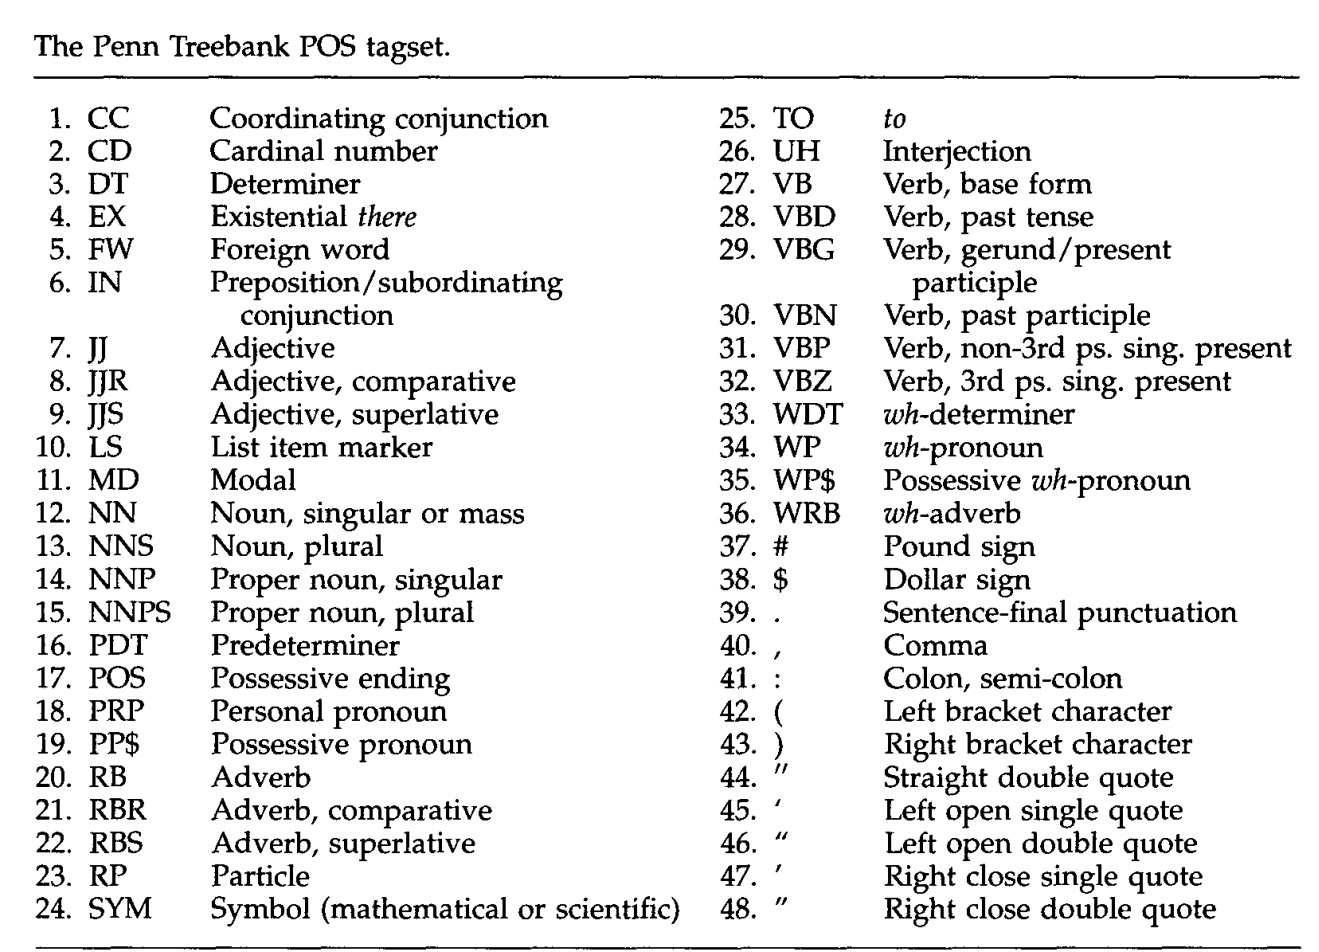
\includegraphics[scale=0.3]{graficos/penn-tagset}
  \caption{Tagset Penn Treebank}
  \label{fig:tagset-penn}
\end{figure}

%\newline

Por su parte, el pos-tagger español de Freeling, por su naturaleza multilingüe, utiliza el tagset propuesto por el grupo EAGLES (\textit{Expert Advisory Group on Language Engineering Standards})\footnote{\url{http://www.ilc.cnr.it/EAGLES96/home.html}}, una organización europea que fomenta la investigación multilingüe, mientras que por una cuestión de compatibilidad, se preservan los tags de Penn Treebank para el inglés. Los tags de EAGLES tienen en consideración diferentes matices para contemplar las variaciones de diferentes idiomas. Sobre un conjunto inicial de 12 categorías -las 9 recién enunciadas más \sq{Signos de puntuación}, \sq{Numerales} y \sq{Fechas y horas} define etiquetas mucho más especificas. En concreto, un tag consta de entre 6 y 7  posiciones, cada una de las cuales expresa una caracteristica de la palabra dependiendo del valor especificado en la posición anterior. Para algunas clases alguno de estos valores no tienen sentido, mientras que para algunas palabras algunos valores no están o no pueden definirse (en el caso de subespecificación de un atributo, esta se nota como un \sq{0}). 
A continuación presentamos la especificación para el conjunto de tags relacionados con sustantivos y un ejemplo de su aplicación.

\begin{center}
\begin{tabular}{| l | l | l | l |}
 \hline
 \multicolumn{4}{|c|}{Nombres} \\ \hline
Pos. & Atributo & Valor & Código \\ \hline
1 & Categoría &  Nombre & N \\ \hline
\multirow{2}{*}{2} & \multirow{2}{*}{Tipo} & Común  & C \\ \cline{3-4}
  & &      Propio & P \\ \hline
\multirow{3}{*}{3} & \multirow{3}{*}{Género} & Masculino & M \\ \cline{3-4}
 & & Femenino &  F \\ \cline{3-4}
 & & Común    & C  \\ \hline
\multirow{3}{*}{4} & \multirow{3}{*}{Número} & Singular & S \\ \cline{3-4}
 & & Plural &  P \\ \cline{3-4}
 & & Invariable & N  \\ \hline
 \multirow{4}{*}{5-6} & \multirow{4}{*}{Clasificación Semántica} & Persona & SP \\ \cline{3-4}
 & & Lugar &  G0 \\ \cline{3-4}
 & & Organización &  O0 \\ \cline{3-4}
 & & Otros & V0  \\ \hline
\multirow{2}{*}{7} & \multirow{2}{*}{Grado} & Aumentativo  & A \\ \cline{3-4}
  & & Disminutivo & D \\ \hline
\end{tabular}
\end{center}


\begin{center}
\begin{tabular}{| l | l | l |}
 \hline
Forma & Lema & Etiqueta \\ \hline 
chico & chico & NCMS000 \\ \hline
chicas & chico & NCFP000 \\ \hline
gatito & gato & NCMS00D \\ \hline
oyente & oyente & NCCS000 \\ \hline
oyentes & oyente & NCCP000 \\ \hline
cortapapeles & cortapapeles &NCMN000 \\ \hline
tesis & tesis & NCFN000 \\ \hline
Barcelona & barcelona & NP000G0 \\ \hline
COI & coi & NP000O0 \\ \hline
Pedro & pedro & NP000P0 \\ \hline
\end{tabular}
\end{center}


Existen varios enfoques algoritmicos al problema del POS tagging: desde los más primitivos basados en reglas escritas a mano pasando a los basados en HMMs (Hidden Markov Models), Maximum Entropy o Transformation Based Learning. Un detalle de estos métodos excede la introducción al problema que supone esta sección de la tesis. El POS tagger de Freeling está basado en el approach de HMMs y el de Stanford en el de Maximum Entropy, ambos modelos de machine learning. En \allref{subsec:freeling-pos} y \allref{sec:stanford-pos} se encuentran algunos comentarios más técnico de los algoritmos de POS tagging que utilizamos en este trabajo y vinculos a bibliografía pertinente y en la sección siguente \allref{subsec:nerc} veremos una descripción más detallada de enfoques algorítmicos al problema que ilustrarán, al menos de modo general, la estructura de la algoritmía basada en machine learning aplicada a procesamiento de lenguajes. 
A continuación listamos ejemplos concretos de análisis de la oración de ejemplo del comienzo de esta sección (\dq{El hombre bajó la escalera.}) para mostrar un funcionamiento real de los algoritmos utilizados en esta tesis. 


\begin{center}
\begin{tabular}{| l | l | l |}
\hline
\multicolumn{3}{|c|}{Freeling (ES)} \\ \hline
Forma &  Etiqueta & Descripción \\ \hline 
El & DA0MS0 & Determinante, Artículo, Másculino, Singular\\ \hline 
hombre & NCMS000 & Nombre, Común, Másculino, Singular  \\ \hline 
bajó & VMIS3S0 & Verbo, Principal, Indicativo, Pasado, Tercera Persona, Singular\\ \hline 
la & DA0FS0 & Determinante, Artículo, Femenino, Singular\\ \hline 
escalera& NCFS000 & Nombre, Común, Femenino, Singular \\ \hline 
.& Fp& Punto final\\ \hline \hline
\multicolumn{3}{|c|}{Freeling (EN)} \\ \hline
Forma & Etiqueta & Descripción \\ \hline 
The &DT & Determiner \\ \hline 
man &NN & Noun, singular or mass \\ \hline 
came  &VBD& Verb, past tense\\ \hline 
down  &RP& Particle \\ \hline 
the &DT& Determiner \\ \hline 
stairs & NNS& Noun, plural \\ \hline 
.& Fp& Sentence final punctuation \\ \hline \hline
\multicolumn{3}{|c|}{Stanford (EN)} \\ \hline
Forma & Etiqueta & Descripción \\ \hline 
The &DT & Determiner \\ \hline 
 man & NN & Noun, singular or mass \\ \hline 
  came &VBD  & Verb, past tense \\ \hline 
 down & RP  &  Particle\\ \hline 
 the & DT  &  Determiner \\ \hline 
 stairs. &NN   & Noun, plural \\ \hline 
 \end{tabular}
\end{center}

En el scope de este proyecto, utilizamos pos-tagging para filtrar clases de palabras inútiles y para seleccionar tres tipos: las qwords, los verbos y los sustantivos (Las qwords son los pronombres interrogativos: qué, quién, cómo, etc. y en inglés, who, when, where...). \newline


\subsection{Reconocimiento de Entidades Nombradas (NER)}
\label{subsec:nerc}

El reconocimiento de entidades nombradas (NER, de Named Entity
Recognition) es una subtarea de Information Extraction. Information
Extraction es, brevemente, todo el dominio de problemas vinculado con
la extracción de información estructurada a partir de datos no
estructurados o semi estructurados. NER es, dentro de este dominio, el
proceso de reconocer unidades de información (las entidades
nombradas) tales como nombres de personas, organizaciones, lugares,
expresiones numéricas como tiempo, fechas, dinero, porcentajes, etc.
A veces se habla de NERC (Named Entity Recognition and Classification)
para poner énfasis en la asignación de un tipo (por ejemplo: nombre
de empresa) a la entidad nombrada reconocida.

Los primeros sistemas de NER eran algoritmos basados en reglas
hardcodeadas, mientras que los más modernos incorporan técnicas de
machine learning y son, en general, algoritmos basados en features.

El primer sistema data de 1991 y constaba de reglas escritas a mano y
heurísticas simples. Recién en 1996, con el estímulo de la MUC-6
(una conferencia reconocida en el área que dedicó una edición a
NER), el área comenzó a acelerar su crecimiento.

Muchos trabajos sobre NER están basados sólo en inglés, pero también existen trabajos para otros idiomas y, más en general, que buscan la independencia del idioma (o también ser multi-idioma). En la CONLL-2003 (otra conferencia reconocida del área) se trabaja fuertemente el problema NER para el alemán, mientras que en la CONLL-2003 se estudia el español y el holandés y, en general, el estado de arte tiene avances, más o menos prometedores, para una gran variedad de idiomas.

El problema del reconocimiento de entidades nombradas está acotado a lo que el filósofo del lenguaje Saúl Kripke llamó “designador rígido”, dejando afuera las descripciones definidas. Por ejemplo, podemos referirnos a Saúl Kripke como “Saúl Kripke” o como “el filósofo de lenguaje que acuñó el concepto de designador rígido”. El primer ejemplo es un designador rígido y un NER debería detectarlo, mientras que el segundo es una descripción y por lo tanto queda afuera de esta subtarea. Notar que ambos denotan unívocamente a un individuo. Para identificar a la compañía automotriz creada por Henry Ford, dos designadores rígidos son “Ford” y “Ford Company”, etc. Más en general, los designadores rígidos incluyen nombres propios tanto como clases naturales (por ejemplo, especies de biología y nombres de sustancias, etc). Además, se incorpora al problema la detección de expresiones temporales (“26 de Agosto de 2013”) y ciertas expresiones numéricas como dinero (“U\$D 250”) y otros tipos de unidades (“20\%”, “10,25”, etc). En un principio se buscaba detectar nombres propios en general, pero luego se incorporó la clasificación como un paso de esta subtarea. Las clases más utilizadas, por una cuestión completamente pragmática, son: persona, organización y lugar (location). Estas tres clases se conocen con el nombre de ENAMEX. A su vez, existen trabajos que subclasifican estas tres clases, dando como output, para un lugar (location), un subtipo como  “ciudad”, “estado” o  “país” y para personas alguna definición más específica (“político”, “farandulero”, “deportista”, etc). Algunos trabajos incluyen otras clases como “varios”, para aquellos que no caen con un grado alto de confiabilidad en ninguna categoría, y categorías específicas para los valores numéricos (date, time, money, percent, etc). Las categorías estándar pueden, sin embargo, adaptarse a las clases de entidades nombradas de un dominio de problemas puntual, pero por lo general este enfoque requiere del entrenamiento de módulos de machine learning, lo cual suele requerir una serie de inputs de los que no siempre se dispone (principalmente, un corpus de datos suficientemente grande para entrenar el sistema y la disponibilidad temporal para configurarlo).


Además de los ya mencionados sistemas de reconocimiento de entidades nombradas basados en reglas escritas a mano del comienzo de las investigaciones en el área, existen los basados en machine learning, en los cuales vamos a detenernos brevemente en esta sección. Los algoritmos basadon en machine learning son entrenados sobre un corpus de datos con ejemplos positivos y negativos de entidades nombradas, a partir de los cuales infieren sus propias reglas de reconocimiento basadas en features. Hay tres tipos de enfoques al problema basados en machine learning: aprendizaje supervisado , aprendizaje semi supervisado y aprendizaje no supervisado.
El aprendizaje supervisado es la técnica actualmente más utilizada para resolver el problema de reconocimiento de entidades. Estos métodos incluyen Hidden Markov Models (HMM), Decision Trees, Maximum Entropy Models (ME), Support Vector Machines (SVM)  y Conditional Random Fields (CRF). Estos métodos son variantes de un modelo único de aprendizaje supervisado que consiste en leer un gran corpus de datos anotados, crear features de identificación y clasificación de entidades a partir de estos datos (generar un \textit{modelo entrenado}) y finalmente identificar y clasificar un input nuevo en base a este modelo. 

En cuanto al aprendizaje semi supervisado, la principal técnica aplicada a NER es conocida como “bootstraping” e involucra un grado de supervisión bajo, como por ejemplo, configurar un conjunto inicial de semillas (seeds) para el algoritmo de aprendizaje. Un ejemplo típico de este tipo de enfoque puede verse en el algortimo {\color{red} KnowItAll?? explicado en la sección Relation Extraction}. Más genéricamente, un algoritmo de aprendizaje semi automático podría buscar a partir de los ejemplos iniciales (dados manualmente) otras entidades que cumplan el mismo rol léxico en contextos similares, para luego iterar sobre el conjunto ampliado.
Otro enfoque consiste en aplicar una serie de reglas simples basadas en patrones (por ejemplo: “New York” es una entidad de tipo location; si empieza con “Sr.” es una entidad de tipo person”) y luego identificar contextos de uso común sobre un corpus para generar reglas basadas en contextos. Un contexto puede incluir desde el rol semántico de las palabras en cuestión hasta ciertos patrones (como por ejemplo “empezar con ‘Sr.’”).

Finalmente, existen algortimos de reconocimiento de entidades basados en aprendizaje no supervisado. El enfoque típico es el clustering, por ejemplo: agrupar entidades nombradas de diferentes clusters basados en similaridad de contexto.  La forma general consiste en aplicar diferentes recursos léxicos (por ejemplo, Wordnet) sobre patrones léxicos y estadísticas tomadas de un gran corpus no anotado. 

En nuestro trabajo utilizamos los NER taggers de Stanford\cite{NER2} y de Freeling, el primero implementando un algoritmo CRF, es decir, de aprendizaje supervisado (ver \allref{sec:stanford-both}) mientras que el segundo es un algoritmo trivial basado en Autómatas Finitos (ver \allref{subsec:freeling-mods}). Para descripciones y referencias de diferentes implementaciones de algoritmos de NERC ver \cite{NER1}.


\subsection{Clasificación de Preguntas (QC)}
\label{subsec:qc}
Question Classification es la tarea de categorizar preguntas en diferentes 
clases semánticas que impongan restricciones significativas a las respuestas potenciales 
para utilizarlas en fases posteriores del proceso de QA.
La clasificación de preguntas es una subclase del problema de la clasificación. 
Un clasificador es una herramienta que asigna a un elemento una de
\textit{k} clases. La clasificación es un área bastante fecunda de nlp y, más en general, de machine learning. 
Los clasificadores de preguntas son herramientas que clasifican preguntas según su tipo de respuesta esperada. Por ejemplo:
\dq{?`Quién descubrió América?} espera, más allá del nombre concreto, \textit{un nombre de persona}; {\textquotedblleft}?`Cuándo se descubrió
América?{\textquotedblright} espera \textit{una fecha} (o, más en
general, \textit{un tiempo}), {\textquotedblleft}?`Dónde se
descubrió América?{\textquotedblright} espera, como respuesta,
\textit{un lugar}, etc. Este es un eje de clasificación conocido como
tipo de respuesta esperado, aunque existen otros. Notar que este último ejemplo, en concreto confuso (¿tiene sentido la pregunta?), no lo es a nivel estructural.

El rol del módulo de QC en un sistema de QA es doble: Por un lado, impoen restricciones a la respuesta final, permitiendo filtrar y verificar respuestas candidatas.
Por otra lado, provee información para estructurar el flujo de código de los procesos subsiguientes, permitiendo implementar estrategias puntuales para cada tipo de respuesta esperada. Por ejemplo, para la pregunta \dq{?`Quién fue el primer presidente constitucional de Argentina?} resulta de gran utilidad, a la hora de evaluar pasajes, saber que la respuesta esperada debe ser una \textit{persona}: de este modo se puede evitar el procesamiento lingüístico de un gran dominio de pasajes no relevantes. Estas mismas razones justifican la deseabilidad de la especificidad: saber que la respuesta final debe ser un \textit{presidente} o un \textit{político} es más informativo y útil para el resto del proceso que solo saber que es una \textit{persona}.

Debido a la complejidad de análisis lingüístico intrinseca en la clasificación específica, los sistemas de QC más básicos adoptan un esquema de clases acotado y basado en reglas simples. Típicamente, las clases son: \textit{Persona}, \textit{Lugar}, \textit{Organización}, \textit{Fecha}, \textit{Cantidad}, \textit{Duración}, \textit{Medida}, mientras las reglas de clasificación son parecidas a las siguientes:
\begin{itemize}
\item Si la pregunta empieza con \textit{Quién} o \textit{Quiénes}, entonces el tipo es \textit{Persona}
\item Si la pregunta empieza con \textit{Dónde}, entonces el tipo es \textit{Lugar}
\item Si la pregunta empieza con \textit{Cuándo}, entonces el tipo es \textit{Fecha}
\item Si la pregunta empieza con \textit{Qué}, entonces determinar el tipo de acuerdo al sustantivo principal de la pregunta (utilizando pos-tagging)
\item ...
\end{itemize}

Como nota al pie, este esquema de clasificación semántico es uno entre otros. Por ejemplo, \cite{QC-other} propuso un esquema \textit{conceptual} de 13 clases en las que incluye, por ejemplo: antecedentes y consecuencias causales, habilitación, verificación, disyunción, etc.

Estas reglas básicas -triviales, si se quiere- cubren gran parte de las preguntas con una eficacia alta. En \allref{sec:stanford-qc} veremos un enfoque más complejo que permite una clasificación más granular, basado en machine learning. El uso de algoritmos de machine learning tiene una serie de ventajes interesantes a la hora de definir un sistema de clases complejo. Como mencionamos al hablar de los otros taggers, la definición de reglas manuales es una tarea tediosa y con poca capacidad de adaptarse o modificarse, mientras que la definición de un set de features adecuado para el aprendizaje programático, en cambio, permite la fácil incorporación de nuevas clases y/o la incorporación de nuevas mejoras descubiertas. Por otro lado, un esquema de clases semánticamente rico -más granular que el modelo básico recién enunciado- requiere la consideración de una gran cantidad de dimensiones lingüísticas, tanto sintácticas como semánticas, lo que hace que la definición manual de reglas una tarea potencialmente imposible en terminos de costo de tiempo humano. 

Finalmente, cabe mencionar que no existen clasificadores de preguntas para el español y que a la hora de abordar este problema en nuestra implementación debimos apelar a mecanismos ad-hoc. En particular, para el modelo estructurado implementamos un sistema de reglas simples como el recién enunciado y para el modelo no estructurado utilizamos el resultado de la clasificación de la misma pregunta pero formulada en inglés (pues las preguntas están disponibles en ambos idiomas).
Actualmente, un tesista del grupo GALLI está trabajando en la construcción de un corpus para alimentar un clasificador de preguntas basado en machine learning para el español, pero lamentablemente por cuestiones de tiempos no pudimos hacer uso del mismo en esta tesis.


\subsection{Otras tareas}

Algunas tareas conocidas de procesamiento de lenguajes que no fueron utilizadas en esta tesis pero que son parte de la \sq{caja de herramientas} con las que podemos encarar problemas que requieran análisis lingüísticos: detección de idiomas, tokenización y particionamiento de textos en oraciones (estas en realidad sí la usamos), resolución de correferencias (por ejemplo: en \dq{Nietzsche murió en 1900. Antes de morir, él estuvo aquejado de una enfermedad mental degenerativa}, \textit{él} refiere a \textit{Nietzsche}), generación de árboles sintácticos y de dependencias, codificación fonética, anotaciones basadas en recursos léxicos (como Wordnet), desambiguación de sentido de palabras (Word sense disambiguation), extracción de relaciones (por ejemplo, para \dq{Nietzsche murió en 1900.} extraer la relación \textit{morir(Nietzsche, 1900)}) y traducción automática (o machine translation). 

\chapter{Estado de Arte}
\label{chap:estado-de-arte}
\section{Introducción general}
\label{sec:intro-general-qa}
\cerrada
Como vimos brevemente en la introducción, QA es un área de investigación de ciencias de la computación que busca generar respuesta concretas a preguntas expresadas en algún lenguaje natural. Es, por esto mismo, un problema complejo que involucra herramientas y modelos de otras áreas de existencia autónoma, como information retrieval (IR), procesamiento del lenguaje natural (PLN, NLP) e information extraction (IE). 

También señalamos algunos ejes de subclasificación de problemas de QA. Con respecto al dominio de hechos y conocimientos sobre los que se espera que el sistema sepa responder los sistemas se clasifican como de dominio abierto (\textit{open domain}) o de dominio cerrado (\textit{closed domain}): mientras de los primeros se espera que sepan responder pregunta acerca cualquier tema o dominio, de los segundos solo se espera que sepan responder preguntas acerca de un dominio acotado particular. A su vez, los datos pueden ser estructurados, semi estructurados o no estructurados. El ejemplo típico de una base de conocimientos estructurada es una base de datos relacional, un tipo de datos semi estructurados puede ser un documento xml no normalizado, mientras que el tipo de datos no estructurado por antonomasia es un corpus de documentos en texto plano. 

Las bases de conocimiento de los sistemas de QA pueden tener uno o más tipos de datos, pero cada unos de estos tipos determina un enfoque algorítmico diferente. Por ejemplo, si la base de conocimientos es una DB relacional con un lengueja formal de consultas similar al SQL, el problema de QA típico consiste en encontrar un mappeo desde la pregunta en lenguaje natural a una consulta formal expresada en un lenguaje comprensible para la base de datos. Esto implica que el foco de trabajo está en la generación de esta consulta y no en el trabajo posterior sobre los resultados de ejecutarla. Por otro lado, un corpus no estructurado no permite una consulta formal, por lo que el enfoque usual es obtener una lista de documentos relevantes para luego aplicar distintas técnicas de procesamiento de textos para extraer la respuesta buscada. 

Estos dos ejes de clasificación (grado de especificidad del dominio y grado de estructuración de los datos) suelen tener una correlación, a saber: los dominios cerrados suelen disponer (o permitir la construcción sencilla de) una base de conocimientos estructurada, mientras que los dominios abiertos suelen forzar datos no estructurados. Esta correlación no es una asociación. En realidad, muchos sistemas open domain actuales son hídridos para estas clasficaciones, ya que suelen combinar varias bases de conocimiento de distintos tipos. Un sistema híbrido podría tener un corpora no estructurado basada en la web para preguntas generales y, a su vez, varias bases estructuradas para dominios especificos, que permiten responder solo algunas preguntas con un resultado mejor. Otro uso puede ser extraer respuestas mediante métodos de pln sobre corpora no estructurados para luego verificar su tipo contra bases de conocimiento estructuradas generales como Freebase o dbPedia. 

En cuanto a aplicaciones comerciales masivas, podemos mencionar la aplicación Siri, el asistente personal de iOS y también la incorporación de funcionalidades de question aswering en los grandes buscadores\footnote{Buscar, por ejemplo: \dq{¿Cuándo nació Bill Gates?} en Google}.  Otros proyectos relativamente actuales que podríamos mencionar son Wolfram|Alpha\footnote{\url{www.wolframalpha.com}}, un sistema online de question answering lanzado por la compañía Wolfram Research y también a IBM-Watson, el sistema de IBM que venció a los favoritos del show de trivia estadounidense Jeopardy!

La organización de este capitulo es como sigue: en lo que queda de esta sección (\allref{sec:intro-general-qa}), repasaremos la historia de la disciplina, desde sus origenes hasta el estado actual de las competencias en torno a las cuales está hoy estructurada la investigación (\ref{subsec:historia}), luego reseñaremos las métricas utilizadas por estas competencias a la hora de evaluar la performance de los sistemas (\ref{subsec:metricas}). En la siguiente sección (\allref{sec:literatura}) pasaremos revista de diferentes investigaciones actuales sobre question answering para definir un modelo más o menos estándar del dominio de problemas y los acercamientos típicos, discutiendo diferentes investigaciones sobre QA open-domain (\ref{subsec:open-domain}), un enfoque estructurado para dominios cerrados (\ref{subsec:closed-domain}) y, finalmente el caso concreto de la implementación de IBM-Watson (\ref{subsec:ibm-watson}) y de otros sistemas  (\ref{subsec:otros-sistemas}).


\subsection{Historia y Competencias}
\label{subsec:historia}
\label{subsec:competencias}
\cerrada
Los primeros sistemas que podemos considerar como pertenecientes al área datan de los años sesenta. Las primeras décadas de investigación al respecto están centradas en sistemas de dominio cerrado, es decir, su objetivo consiste en responder preguntas sobre temas específicos, apoyandose en general en una base de conocimientos estructurada, especificamente creada para el sistema. Por ejemplo Baseball \cite{BASEBALL}, un proyecto del MIT que data de 1961, es la primera investigación académica cuyo enfoque la incorpora con certeza en este área que pudimos encontrar en Internet. Baseball respondía preguntas sobre algunos hechos vinculados al torneo de la Liga Americana de baseball de un año (no se especifica cuál). La información se archivó de manera estructurada y contenía: el día, el mes, el lugar, los equipos y los puntajes de cada juego por un año\footnote{Como una nota de color, trascribimos las dos primeras oraciones del abstract: \dq{Baseball is a computer program that answers questions phrased in ordinary English about stored data. The program reads the question from punched cards}. Traducido: Baseball es un programa de computadora que responde preguntas verbalizadas en inglés común sobre datos guardados. El programa lee la pregunta de tarjetas perforadas.}. Otro ejemplo conocido es el chatbot-psicóloga Eliza, cuyo código original fue escrito en 1966, que se basa en reglas muy simples de matcheo de las lineas ingresadas por el usuario para simular una conversación de terapia bastante convincente\footnote{En internet están disponibles diferentes implementaciones de Eliza. En \url{https://github.com/julian3833/eliza} puede encontrarse una implementación funcional en python}. Existieron otros desarrollos e investigaciones durante las siguientes décadas, con complejidad creciente, pero con un enfoque similar al de Baseball y de Eliza. Pero la investigación, la producción de software y, principalmente, la formación de una comunidad de desarrollo e investigación mínimamente articulada vinculada con el question answering estuvo impulsada fuertemente por el lanzamiento de los ejercicios de QA en la competencia TREC\footnote{\url{http://trec.nist.gov/}} (Text Retrieval Conference) en el año 1999, la TREC-8 \cite{TREC8}.

TREC se convirtió en una referencia obligada y centro de nucleamiento de la investigación en QA. Esta primera competencia monolengua (para inglés), consistía en retornar un fragmento de texto de entre 50 y 250 bytes conteniendo la respuesta a preguntas fácticas (factoids). La evaluación, que marcó la historia futura de la evaluación de QA en competencias, consideraba el sistema de QA como un todo, es decir, no consideraba la evaluación de subcomponentes. La organización permitía dar una lista con 5 respuestas posibles por cada pregunta, y esto siguió así hasta la TREC-2002, cuando se comenzó a exigir una sola respuesta por pregunta. TREC siguió lanzando un track de QA en todas sus competencias anuales, variando la forma y la complejidad de los ejercicios propuestos, por ejemplo: incorporando preguntas largas, con un formato realista y corpora de mayor tamaño, también introduciendo preguntas sin respuesta (NIL answers) y preguntas de tipo Lista (por ejemplo: \sq{¿Qué libros escribió Friedrich Nietzsche entre 1870 y 1896?}), pregunta de definiciones (por ejemplo: \sq{¿Quién es el General Paz?}), en TREC 2003, preguntas agrupadas por un tema (target), explícito o implícito y de diferentes tipos -como personas, organizaciones, cosas, eventos, etc-, restricciones temporales (por ejemplo: antes, durante y después de una fecha, evento o período), anáforas y co-referencias entre preguntas (por ejemplo: ¿Quién es George Bush?. ¿Y quién es \textit{su} esposa?), etc. Las competencias anuales de la TREC, por otro lado cambiaron el enfoque que existía en décadas anteriores, hacia preguntas de dominio abierto y corpora de datos textuales planos. 

En lo que respecta a los sistemas multi-idioma (y mono-idioma no centrados en inglés), más allá de algunos eventos anteriores, un hito clave es el lanzamiento, en 2003, de la primer tarea de QA \cite{CLEF03} de CLEF (Cross Language Evaluation Forum)\footnote{\url{http://www.clef-initiative.eu/}} proponiendo ejercicios tanto monolingües como multilingües en varios idiomas europeos. Se propusieron ejercicios monolingües para francés, español, alemán, italiano y neerlandés, y ejercicios multilingües, con corpora en inglés y preguntas en otros idiomas europeos. En este año, se exigían respuesta de hasta 50 bytes, se permitía una lista de 3 respuestas por pregunta y los ejercicios podían incluir preguntas sin respuesta en los corpora. En la CLEF 2004, la tarea de QA principal incorporó 9 lenguas de origen (lengua de la pregunta) y 7 de destino (lengua del corpus), habilitando 55 ejercicios mono y bilingües. La cantidad de respuesta se redujo a 1 y se incorporaron preguntas de tipo "¿Cómo...?", de definiciones, de listas y también se agregaron restricciones temporales (antes, durante y después de una fecha, evento o período). CLEF continuó presentando pistas de ejercicios de QA todos los años desde entonces, con diferentes variaciones. Otra conferencia de prestigio en el área es NTCIR \footnote{\url{http://research.nii.ac.jp/ntcir/}}, que puede es un análogo a CLEF para idiomas asiáticos, incorporando tareas monoligües y bilingües entre inglés, japonés y chino, entre otras.

\subsection{Métricas de evaluación}
\label{subsec:metricas}

En cuanto a las métricas de evaluación utilizadas por estas competencias respecta, es importante distinguir la evaluación de las respuestas a una pregunta y la evaluación general del sistema. Con respecto a la evaluación de respuestas, la clasificación usual de evaluación consiste en 4 valores asignados a cada respuesta: Correcta (C), si responde a la pregunta y el fragmento de soporte justifica esa respuesta; No soportada (U, de Unsupported), si responde a la pregunta pero el fragmento de soporte no está o no justifica la respuesta; Inexacta (X), si sobra o falta información en la respuesta (algunas campañas solo aceptan respuestas exactas) y, finalmente, Incorrecta (I), si ninguna de las condiciones anteriores se cumple. 

La evaluación de respuestas puede ser estricta (strict) o \textit{indulgente} (lenient) dependiendo de si considera las respuestas no soportadas como válidas o como inválidas. Por otro lado, la evaluación puede ser manual -llevada a cabo por un jurado especial- o bien automática. En el caso de la evaluación automática, siempre es indulgente, ya no hay forma de decidir si un fragmento soporta o no una respuesta. Para este tipo de evaluaciones se suele utilizar un set de patrones de respuestas correctas que se deriva de un set de "respuestas conocidas" generadas por los organizadores y los mismos competidores, conocido como R-set, pero no es un proceso trivial: en principio, es dificil saber qué respuestas correctas puede esperarse, ya que por la naturaleza del problema es probable que diferentes sistemas devuelvan respuestas textualmente distintas. 

Con respecto a la métricas de evaluación para sistemas como un todo, veremos a continuación las métricas másconocidas: MRR (Mean reciprocal rank, o promedio de rankings recíprocos), CWS (Confidence Weighted Score, Puntaje ponderado por confiabilidad) y K-Measure (Medida K).

\subsubsection*{MRR Mean Reciprocal Rank}
El MRR mide la habilidad de un sistema para responder un conjunto de pregunta $Q$. Asume que el sistema devuelve una o más respuestas por pregunta, en orden de "confiabilidad". El puntaje de cada pregunta individual ($RR(q_i)$) se define como la inversa de la posición de la primera respuesta correcta en la lista de respuestas dada, o cero si no hay ninguna.

\begin{equation}\label{eq:precision}
 \text{MRR} = \frac{1}{|Q|} \sum_{i=1}^{|Q|} \frac{1}{RR(q_i)}. \!
\end{equation}

\begin{equation*}
    RR(q_i) = \begin{cases}
               0     & \text{si existe al menos una respuesta correcta}\\
               \frac{1}{\text{Posicion de }q_i} & \text{si }q_i\text{ es la primer respuesta correcta}\\
           \end{cases}
\end{equation*}

MRR puede tomar valores entre 0 y 1 inclusive, aunque el RR de cada pregunta tiene un espectro finito de valores (por ejemplo, para 5 respuestas puede valer 0, 0.2, 0.25, 0.33, 0.5 o 1). La primera vez que se usó MRR fue en la competencia TREC-8. En esa competencia se permitía una lista de 5 respuestas ordenadas para cada pregunta.  


\subsubsection*{“Confidence Weighted” Score}
“Confidence Weighted” Score, (CWS, also known as 
Average Precision) was defined for TREC-11 and is inspired 
from Document Retrieval’s uninterpolated average precision. 
Assuming exactly one possible answer by question (from a Q 
set), and that all these answers must be ordered by system’s 
confidence in its response, CWS rewards correct answers 
placed earlier more than later one. It is defined as: 


\begin{equation}\label{eq:recall}
  \mbox{Recall}=\frac{|\{\mbox{documentos relevantes}\}\cap\{\mbox{documentos recuperados}\}|}{|\{\mbox{documentos relevantes}\}|} 
\end{equation}

% 1
% 1
% (number correct in first ranks)
% Q
% i
% CWS i
% Q =
% = ∑
 
CWS ranges between 0 (no correct at all) and 1 (perfect 
score). It was abandoned because it was inappropriate due to 
changes in the TREC-12 track definition, but also because, it 
could reward QAS ordering answers strategies rather than 
their correctness to answer. 

\subsubsection*{K-Measure}
K-Measure was designed at CLEF 2004’s Pilot Task 
(Herrera et al., 2004) for rewarding systems “that return as 
many different correct answers as possible to each question, 
but at the same time, punishing incorrect answers”. It needs 
as a prerequisite a “self” confidence score, between 0 and 1, 
for each answer candidates. K-Measure is defined as follows: 
% 1 { }
% ( ) ( ) 1
% max ,
% i
% Q
% a sysAnswers
% i i i
% confidence a judgement a
% K
% Q R sysAnswers
% ∈
% =
% ⋅
% =
% ∑
% ∑
 
where, for a question i: Ri 
is the set of correct answers; 
sysAnswersi
 is the set of answer candidates (a); confidence(a) 
is the confidence score given by QAS to an answer; and 
judgement(a) is the judgment given by an human assessor 
valued between {1, 0, -1} respectively for an answer judged 
correct, for an answer already judged, and for an incorrect 
one. K-Measure is ranged between 0 (no evidence of 
correctness) and 1 (certainty of correctness). As authors 
pointed out, the main difficulty is still determining an 
exhaustive Ri
 set for each question. So, they propose an 
alternative, called K1-Measure, when only one single answer 
is admitted per question. It assumes Ri
 can be approximated 
by the Known set of correct answers. K1 is defined like 
K-measure without the recall part (the “maximum” 
denominator). Also, to have better clues on correlation 
between self-scoring confidence and assessors judgment 
correctness, they defined a correlation coefficient called r. 

\subsubsection*{Otros}
List Questions or measuring many answers at the same 
time: Expected answers (instances) to List questions 
constituted a closed set usually assembled from many 
documents. It can be evaluated using Accuracy, i.e. the ratio 
of distinct correct answers to target number of instances; or 
even with Recall, Precision and F-Measure since the R-set is 
actually exhaustive for these questions. Last possibility is to 
adapt the Non-Interpolated Average Precision (NIAP) 
measure borrowed to Document Retrieval community and 
defined as: 
% 1 { ' | ' , ( ') ( )}
% ( )
% i
% i
% i a R
% a a R rank a rank a
% NIAP
% R rank a ∈
% ∈ ≤
% = ∑
 
where, for a question i: Ri 
is the set of correct answers; 
and rank(a) is the rank of an answer in the (ordered) answer 
candidates to evaluate. 


Measures for Definition Questions. Such questions pose 
a problem: they accept many possible correct answers, but all 
will not be accurate or interesting, from a user’s point of 
view (profiled as “an adult, a native speaker of English, and 
an average readers of ‘US’ newspapers”). Therefore, since 
recent evaluations, assessors built a by pipelining many 
processing list of vital nuggets of information, a QAS should 
return to a Definition question (Voorhees, 2003). Using this 
list, questions can be manually evaluated at a conceptual 
level (to abstract vocabulary, syntactic and others paraphrases 
mismatches). Recall, Precision (depending on an allowance 
length score to penalize verbosity) and F-measures are then 
computed. 
(Lin and Demner-Fushman, 2005) and recently (Marton, 
2006) proposed automatic metrics to replace this final 
manual evaluation. First authors, presented a measure, traced 
from ROUGE measure - (Chin-Yew and Hovy, 2003) used in 
automatic document summarization - which made the same 
assumption that the term co-occurrence statistics (unigrams) 
can replace the manual semantic matching process. They 
showed that their metrics highly correlate with TREC 
assessors’ evaluation. Marton, echoed and investigated 
further to better approximate assessment score. His method 
used binary classifiers, based on up to trigrams, using 
function of an idf-based weight, an informativeness score and 
a recall threshold. He showed many improvements such as 
interpretable score, a confidence interval, exactly reproducing 
already done human assessments, better accuracy through 
additional annotation and support for using judgment data.

\section{Literatura y sistemas}
\label{sec:literatura}
\subsection{Enfoques sobre open domain}
\label{subsec:open-domain}

Existe un consenso general a la ahora de definir el modelo de software más abstracto o de arquitectura para encarar la construcción de un sistema de question answering open domain. Esta arquitectura consiste en un pipeline con al menos tres módulos o compotentes bien diferenciados:
\begin{itemize}
\item Módulo de procesamiento de la pregunta
\item Módulo de procesamiento de documentos
\item Módulo de procesamiento de la respuesta
\end{itemize}

Cada uno de estos módulos cuenta a su vez con subcomponentes sobre los cuales hay mayor o menor consenso, que determinan, en definitiva, la performance del sistema concreto implementado. 

El módulo de procesamiento de la pregunta tiene como subcomponente principal un Clasificador de Preguntas (Ver \allref{subsec:qc} y \allref{sec:stanford-qc}) y puede incorporar otros componente como identificadores del \sq{foco} (\textit{focus}) y del tipo esperado de la respuesta (\textit{answer type}), y también puede incluirse en este módulo un componente encargado de expandir o reformular la pregunta para optimizar los resultados del módulo de procesamiento de documentos ( este subcomponente también se suele considerar como parte del módulo de procesamiento de respuestas). Este último subcomponente tiene diferentes nombres en la literatura (\textit{query reformulation}, \textit{query generation}, \textit{query expansion}, etc).

En el núcleo del módulo de procesamiento de documentos, por lo general, hay uno o más índices invertidos (como Lucene o {\color{red} XXX}) como el descripto en \allref{subsec:indice-invertido}, o bien accesos a un buscador web, o, más en general, estructuras de information retrieval. Como vimos (\ref{subsec:metricas-ir}, existen dos métricas fundamentales a la hora de evaluar el funcionamiento de un módulo de information retrieval: precisión y recall. La precisión es la proporción de documentos relevantes devueltos sobre el total documentos devueltos por el módulo, mientras que el recall es la proporción de documentos relevantes devueltos sobre el total de documentos relevantes existentes en la base de conocimientos. Estas dos métricas suelen comportarse una con la otra como un trade-off, es decir: suelen aparecer escenarios de diseño en los que se deberá optar por priorizar una o bien la otra. Considerando esto, existe una tercera métrica extendida, la medida $F$, que busca parametrizar este compromiso. 

En el contexto de uso de los sistemas de QA, la métrica que se busca maximizar para el módulo de procesamiento de documentos es el recall, es decir, no interesa que el módulo no recupere documentos no relevantes siempre y cuando recupere todos los documentos relevantes existentes que pueda. El motivo es simple: se espera que el análisis lingüístico fino del módulo de procesamiento de la respuesta sea capaz de eliminar texto irrelevante en la misma o en mejor medida que el sistema de information retrieval subyacente al módulo de documentos. Por otro lado, si al recuperar los documentos se filtra una respuesta válida como irrelevante, entonces el resto del pipeline vera sus probabilidades de éxito mermadas (sino directamente anuladas).  La expansión/reformulación de la pregunta del paso anterior apunta, justamente, a generar una query que priorice el recall sobre la precisión. O

Otras tareas que se realizan en el módulo de procesamiento de documentos es la división de los documentos en parágrafos, el filtrado de documentos o parágrafos irrelevantes y el ranking de los resultados. Si bien los sistemas de information retrieval suelen rankear sus resultados, este ranking puede resultar no del todo adecuado para la tarea en cuestión y mejorable teniendo en cuenta la información disponible. 

Finalmente, el módulo de procesamiento de respuestas introduce el valor agregado que distingue un sistema de IR típico y un sistema de QA propiamente dicho. Este módulo es el menos estandarizado de los tres y tiene diferentes enfoques más o menos elaborados en la literatura, pero el grado de consenso sobre la viabilidad del uso de un grupo de técnicas fijas sobre otras no ocurre como, por ejemplo, en el uso de un clasificador de preguntas en el módulo de procesamiento de preguntas o de un índice de búsquedas en el módulo de procesamiento de documentos. Típicamente, el módulo consta de tres momentos: a partir de los parágrafos o documentos rankeados generados por el módulo de documentos se busca identificar oraciones o respuestas candidatas mediante distintas técnicas. Para estas respuestas candidatas identificadas, se extrae la información concreta que responde a la pregunta utilizando heurísticas basadas en las etiquetas obtenidas para la pregunta (clase de pregunta, foco, tipo de respuesta, etc). Finalmente, se implementa algún mecanismo de corroboración o de validación de respuestas, generando una respuesta final.

A continuación nos extenderemos con más detalle sobre los tres módulos propuestos señalando algunos enfoques usuales, usando como guía los papers \cite{QA-survey}, \cite{QA1}, \cite{QA2}, \cite{QA3} y \cite{PASSAGE1}.

\subsubsection*{Módulo de procesamiento de la pregunta}
Este módulo recibe como input una pregunta formulada en algún lenguaje natural y genera como output una representación de la misma que resulte útil para los módulos siguientes. Esto suele realizarse agregando labels o etiquetas (ver Features, en \allref{sec:terminologia}) a la pregunta completa y a sus distintos términos.

La etiqueta principal generada es el tipo de pregunta (\textit{question type}) y para obtenerlo se utiliza un clasificador como el que describimos en (\ref|{subsec:qc})· Lamentablemente, la clasificación de preguntas no está desarrollada para otros idiomas que el inglés, al menos, no con el mismo grado de precisión y visibilidad que, por ejemplo, el clasificador de Stanford \cite{QC1} \cite{QC2}. Como vimos anteriormente, el principal problema a la hora de clasificar una pregunta es la ambigüedad intrinseca de ciertas clases de preguntas. 

A partir del tipo de pregunta se define el tipo de respuesta esperada (\textit{answer type}). No existe un algoritmo automático estándar difundido para generar el tipo de respuesta esperado. El enfoque general encontrado es la aplicación de un mappeo simple basado en reglas, desde el tipo de pregunta generado por el clasificador a una serie de tipos de respuestas predefinido para el dominio de problema.

Otro análisis interesante pero, según nuestra investigación, no sistematizado, es el análisis del \dq{foco} (\textit{question focus}). En \cite{QA3} se define el foco como una palabra o secuencia de palabras que indican qué se está preguntando. Por ejemplo, para la pregunta \dq{¿Quién fue nombrado presidente de Argentina en  1983?} el foco sería \dq{presidente}). {\color{red} VER MI RESUMEN DE QA-SURVER, COMENTARIO PERSONAL}. El concepto aparece también en \cite{WATSON1} pero no encontramos detalles sobre los mecanismos técnicos implicados en la extracción y todo parece señalar a una serie de heurísticas de procesamiento lingüístico escritas a mano. 

Otros análisis que se realizan sobre la pregunta son el POS-tagging (Ver \allref{subsec:pos}), el reconocimiento de entidades nombradas (NER, ver \allref{subsec:ner}) y la búsqueda de dígitos u otros patrones útiles para el contexto. 

Finalmente, se ejecuta la reformulación o expansión de la pregunta para genera un input para el módulo de information retrieval tal que maximice el recall. 
La idea guía es la extracción de keywords relevantes y existen diferentes enfoques, usando los pos-tags y el resultado del ner. También pueden utilizarse recursos léxicos como Wordnet para generar sinónimos de términos importante. 

En \cite{QA1} y \cite{QA3} se propone una heurística basada en 8 reglas para implementar este paso. Las reglas propuestas son:

\begin{itemize}
\item {\color{red} Fill me neddy}
\end{itemize}

\subsubsection*{Módulo de procesamiento de documentos}
El input del módulo de procesamiento de documentos es la pregunta reformulada según describimos en los párrafos inmediatamente anteriores y su output es una lista de documentos (o parágrafos) ordenados según la factibilidad de que contengan la respuesta a la pregunta. El módulo consta, en general, de uno o más sistemas de information retrieval (entre los cuales puede estar la web indexada) y de submodulos de filtrado, fragmentación y reordenamiento. Sobrelos sistemas de information retrieval es importante notar que suelen usarse sistemas tradicionales y no aquellos basados en distancias coseno, como el utilizado, por ejemplo, en latent semantic analysis (LSA). Este último enfoque, que demostró ser útil a la hora de eliminar o reducir problemas de {\color{red} qué resuelve LSA} en information retrieval, pero en QA es importante que las keywords de búsqueda mismas estén presentes en los documentos relevantes y no que sean solamente \dq{semánticamente similares}. Dada la gran cantidad de documentos que se espera que retorne el subsistema de information retrieval (como señalamos, se prioriza el recall y no la precisión), existe un paso de filtrado (en \cite{WATSON1} se lo nombra como \sq{soft filtering}) en el cual: 1\textsuperscript{o} se reduce la cantidad de documentos a retornar por el módulo en general y 2\textsuperscript{o} se reduce la cantidad de texto en cada documento. El principio que guía este proceso es la idea de que las palabras clave de la pregunta deben aparecer, de alguna manera, cercanas entre sí. De este modo, es posible buscar por estas keywords en los documentos y quedarse solo con los $N$ parágrafos que contengas las keywords, desechando el resto del texto

{\color{red}Implementación de LASSO??}

Finalmente, se procede a ordenar los parágrafos / documentos filtrados. Una implementación posible de este ordenamiento es utilizar radix sort, considerando los siguientes tres scores. {\color{red} INCONCLUSO}


\subsubsection*{Módulo de procesamiento de la respuesta}
Finalmente, el modulo de procesamiento de respuestas es el encargado de generar una respuesta a partir del output de los otros dos módulos. Para ello debe identificar la respuesta dentro de los parágrafos, extraer la fracción de texto que responde puntual y concretamente a la pregunta y, finalmente, validar su corrección. 

Para identificar la respuesta se utilizan distintas heurísticas, utilizando el tipo de respuesta esperado cuando es posible. Sin embargo, el tipo de respuesta esperado no siempre es explícito en la pregunta o en la respuesta, por lo que se utilizan diferentes reglas basadas en pos-tags, ners, en un parser específico para el reconocimiento de las respuestas candidatas.

Para las respuestas candidatas se extrae luego el o los términos concretos de la respuesta final {\color{red} Por ejemplo: }. Existe sobre este punto heúristicas más o menos avaladas basadas en distancias entre keywords, número de keywords presentes y otras métricas similares (ver, por ejemplo, {\color{red} Qanus, scorers}. Típicamente, si no se encuentra ninguna coincidencia confiable, los sistemas de QA productivos recaen en la devolución de los primeros $n$ parágrafos mejor rankeados por el módulo de documentos. 

Como señalamos anteriormente, en las competencias TREC hasta 2001 se permitía devolver una lista de 5 respuestas, mientras que desde el 2002 se exige una única respuesta.

Finalmente, hay distintas formas de validar la corrección o de estimar un grado de confianza en la corrección de una respuesta. En primer lugar, pueden usarse diferente corpus especificos {\color{red} INCONCLUSO}.

\subsection{QA como interfaz a una base de datos}
\label{subsec:closed-domain}

\subsection{IBM-Watson}
\label{subsec:ibm-watson}
Watson\cite{WATSON1}\cite{WATSON2} es un sistema diseñado por IBM con el objetivo de competir en
tiempo real en el programa de televisión estadounidense Jeopardy,
logrando resultados del nivel de los campeones humanos de este
programa.

El proyecto demoró 3 años de investigación, en los cuales se
logró obtener la performance esperada (nivel humano experto) en
cuanto a precisión, confiabilidad y velocidad, logrando derrotar a
dos de los hombre con mayores récords históricos del show en un
programa en vivo\footnote{En esta url está disponible el programa en el que el sistema vence a sus competidores humanos: \url{http://www.youtube.com/watch?v=WFR3lOm_xhE}} en febrero de 2011.

El objetivo del \ proyecto puede considerarse una extensión de lo que
fue Deep Blue, el sistema que logró el nivel de los expertos humanos
en el ajedrez, porque buscó superar un reto que significativo y
visible del campo de la Inteligencia Artificial tanto para la comunidad
científica como para la sociedad en general:
{\textquotedblleft}?`puede un sistema computacional ser diseñado para
competir con los mejores hombre en alguna tarea que requiera altos
niveles de inteligencia humana y, si es el caso, que clase de
tecnología, algoritmos e ingenieria se
requiere?{\textquotedblright}\footnote{Traducción propia de
un fragmento de \cite{WATSON1}, p. 2}

Watson es la implementación específica para participar en este
programa de una arquitectura más genérica de question answering,
DeepQA, que da el nombre al proyecto de la corporación. Esta
arquitectura es de construcción reciente y ejemplifica perfectamente la complejidad del problema de
QA de dominio abierto e incorpora tecnologías de punta de distintos
dominios de ciencias de la computación, y de IA en particular:
information retrieval, natural language processing, knowledge
representation and reasoning, machine learning e interfaces humano -
computadora. En el transcurso de esta tesis, IBM lanzó el programa
\sq{Watson Ecosystem} (en noviembre de 2013) que promete la utilización
de tecnología de punta para aplicaciones creadas por la comunidad\footnote{
Announcing the IBM Watson Ecosystem Program: \url{http://www-03.ibm.com/innovation/us/watson/}}.

\subsubsection*{El problema}

Watson debe realizar tareas como parsing, question classification,
question descomposition, automatic source adquisition and evaluation,
entity and relation detection, logical form generation, knowledge
representation and reasoning manteniendo ciertos atributos de calidad
bastante exigentes derivados de la naturaleza del show. Estas
restricciones son:

\begin{itemize}
\item Confiabilidad de la respuesta: \newline
Jeopardy tiene tres participantes con un pulsador y el que desee
responder debe pulsar antes que los demás. Además, existe una
penalización por respuestas incorrectas, por lo que es esencial que
el sistema pueda determinar la confiabilidad de la respuesta obtenida a
fin de optar por responder o no responder.
\item Tiempos de respuesta: \newline
La confiabilidad de la respuesta, o al menos una estimación, debe
calcularse antes de que pase el tiempo para decidir responder (6
segundos) y también de que otro participante oprima su pulsador
(menos de 3 segundos).
\item Precisión:\newline
El tipo de respuestas que se dan en el show suelen ser respuestas
exactas (por ejemplo: solamente un nombre, un número o una fecha,
etc). 
\end{itemize}

\bigskip

El sistema cuenta con varios componentes heurísticos que estiman
ciertos features y grados de confiabilidad para diferentes respuestas,
los cuales son evaluados por un sistema general que sintetiza un grado
de confiabilidad para una respuesta final y determina así si
responder o no responder. 

El programa consta de un tablero con 30 pistas (o preguntas) organizadas
en seis columnas, cada una de las cuales es una categoría. Las
categorías van desde temas acotados como
{\textquotedblleft}historia{\textquotedblright} o
{\textquotedblleft}ciencias{\textquotedblright} hasta temas más
amplios como {\textquotedblleft}cualquier cosa{\textquotedblright} o
{\textquotedblleft}potpourri{\textquotedblright}. Watson intenta
respuestas sobre varias hipótesis de dominio y verifica en cual de
ellos se logran respuestas de mayor confiabilidad. 

Por otra parte, el grueso de las preguntas de Jeopardy son del tipo
\textit{factoid}, esto es, preguntas cuya respuesta esta basada en
información fáctica acerca de una o más entidades individuales.


\bigskip

Por ejemplo:

Categoría: Ciencia General

Pista: Cuando es impactado por electrones, un fósforo emite energía
electromagnética de esta forma

Respuesta: Luz (o fotones)


\bigskip

A su vez, existen ciertos tipos de pistas que requieren un enfoque
particular, por ejemplo, pistos que constan de dos subpistas muy
débilmente relacionadas, o problemas matemáticos formulados en
lenguaje humano, o problemas de fonética, etc, que no pueden ser
simplemente dejados de lado porque, si bien tiene poca probabilidad de
aparición, cuando aparecen lo hacen en bloque y pueden arruinar el
juego de Watson. Se acordó con la productora del programa, sin
embargo, dejar de lado preguntas audiovisuales (aquellas que presentan
una imagen o un audio y requieren interpretarlo) y preguntas que
requieren instrucciones verbales del presentador.


\bigskip

Para determinar el dominio de conocimiento, los investigadores
analizaron 20000 preguntas, extrayendo su LAT (lexical answer type, o
tipo léxico de respuesta). El LAT se define como una palabra en la
pista que indica el tipo de la respuesta esperado. Por ejemplo, para la
pista {\textquotedblleft}Investanda en 1500{\textquoteright}s para
agilizar el juego, este movimiento involucra dos
piezas{\textquotedblright} el LAT es
{\textquotedblleft}movimiento{\textquotedblright}. Menos del 12\% de
las pistas no indicaba explícitamente ningún LAT, usando palabras
como {\textquotedblleft}esto{\textquotedblright} o
{\textquotedblleft}eso{\textquotedblright}. En estos casos, el sistema
debe inferir el tipo de respuesta del contexto. Del análisis de estas
20000 pistas se reconocieron 2500 tipos léxicos distintos, de los
cuales los 200 más frecuentes no llegaban a cubrir el 50\% del total
de pistas. Esto implica que un approach estructurado (orientado por el
tipo de respuesta), si bien resulta útil para algunos tipos, no es
suficiente para abordar el problema completo.

\subsubsection*{Métricas}

Las métricas de resultados, además del tiempo de respuesta, son la
\textit{precisión} (preguntas contestadas correctamente / preguntas
contestadas) y el \textit{porcentaje de respuestas dadas }(preguntas
contestadas / total de preguntas). Mediante la configuración de un
threshold de \textit{confiabilidad} pueden obtenerse distintas
estrategias de juego: un umbral bajo repercutirá en un juego más
agresivo, incrementando la proporción de respuestas contestadas,,
pero disminuyendo su precisión, mientras que un umbral alto
determinará un juego conservador, con menos respuestas dadas pero
mayor precisión en las mismas. Es un clásico escenario de trade-off
entre dos atributos de calidad. Un buen sistema de estimación de
confiabilidad implica una mejora general del sistema, aún cuando el
módulo de generación de respuestas permanezca idéntico.


\bigskip

En el show, el porcentaje de respuestas dadas depende de la velocidad
con la que se llega a presionar el pulsador, lo cual sólo interesa
para el dominio de QA como una restricción temporal. 


\bigskip

Mediante análisis numérico, los investigadores determinaron que los
campeones de Jeopardy lograban tomar entre el 40\% y el 50\% de las
preguntas y, sobre ellas, lograban una precisión de entre el 85\% y
el 95\%, lo que determinaba una barrera de performance bastante
exigente en lo que respecta a QA.


\bigskip

\subsubsection*{Baseline}

El equipo de IBM intentó utilizar dos sistemas consolidados en QA y
adaptarlos al problema \ de Jeopardy. \ El primero fue PIQUANT
(Practical Intelligent Question Answering Technology), un sistema
desarrollado por IBM en conjunto con el programa del gobierno
estadounidense AQUAINT y varias universidades, que estaba entre los
mejores según la TREC (Text Retrieval Conference), una autoridad en
el área. PIQUANT consta de un pipeline típico (véase QANUS) con
tecnología de punta, logrando un rango del 33\% de respuestas
correctas en las evaluaciones TREC-QA. Los requerimientos de la
evaluación de TREC son muy distintos de los de Jeopardy: TREC ofrece
un corpus de conocimiento relativamente pequeño (1M de documentos) de
donde las respuestas deben ser extraídas y justificadas, el tipo de
preguntas de TREC son menos complejas a nivel ling\"uístico que las
de Jeopardy y la estimación de confiabilidad no resulta una métrica
importante (dado que no hay penalización por respuestas incorrectas).
Además, los sistemas tienen permitido acceder a la web y las
restricciones temporales son, por mucho, más amplias (por ejemplo:
una semana para responder 500 preguntas). En Jeopardy, además de las
restricciones ya mencionadas, un requerimiento fue que el sistema
trabaje sobre datos locales y no acceda a la web en tiempo real. El
intento de adaptar PIQUANT al problema de Jeopardy dio pésimos en
comparación con los necesarios: 47\% de precisión sobre el 5\% de
respuestas con mayor confiabilidad y 13\% de precisión en general. 

Por otro lado, el equipo intentó adaptar el sistema OpenEphyra
(véase OpenEphyra), un framework open-source de QA desarrollado en
CMU (Carnegie Mellon University) basado en Ephyra (no libre),
diseñado también para la evaluación TREC. OpenEphyra logra un
45\% de respuestas correctas sobre el set de datos de evaluación TREC
2002, usando busqueda web. La adaptación resultó aún peor que la
de PIQUANT (con menos del 15\% de respuestas correctas y una mala
estimación de la confiabilidad). 

Se probaron dos adaptaciones de estos sistemas. una basada en
búsquedas de texto puro y otra basada en reconocimiento de entidades.
En la primera, la base de conocimiento se modeló de manera no
estructurada y las preguntas se interpretaron como términos de una
query, mientras que en la segunda se modeló una base de conocimientos
estructurada y las preguntas se analizaron semánticamente para
reconocer entidades y relaciones, para luego buscarlos en la base.
Comparando ambos enfoques en base al porcentaje de respuestas dadas, el
primero dio mejores resultados para el 100\% de las respuestas,
mientras que la confiabilidad general era baja; por otro lado, el
segundo enfoque logró altos valores de confiabilidad, pero sólo en
los casos en que efectivamente logra identificar entidades. De aquí
se infiere que cada enfoque tiene sus ventajas, en el dominio de
problemas apropiado.

\subsubsection*{La arquitectura DeepQA}
\label{subsec:deep-qa}
Los intentos de adaptación iniciales, como vimos, no dieron
resultados, así como tampoco sirvieron las adaptaciones de algoritmos
de la literatura científica, los cuales son realmente difíciles de
sacar de su contexto original y de las evaluaciones sobre las cuales
fueron testeados. Este problema, veremos -por ejemplo, con QANUS y
Reverb- , se repitió en nuestro proyecto. Como conclusión de estos
intentos frustrados, el equipo de IBM entendió que una arquitectura
de QA no debía basarse en sus componentes concretos sino en la
facilidad para incorporar nuevos componentes y para adaptarse a nuevos
contextos. Así surgió DeepQA, la arquitectura de base, de la cual
Watson es una instancia concreta para un contexto particular (con
requerimientos de alta precisión, buena estimación de
confiabilidad, lenguaje complejo, amplitud de dominio y restricciones
de velocidad). DeepQA es una arquitectura de computo paralelo,
probabilistico, basado en recopilación de evidencia y scoring. Para
Jeopardy se utilizaron más de 100 técnicas diferentes para analizar
lenguaje natural, identificar y adjudicar valor a fuentes de
información, encontrar y generar hipótesis, encontrar y rankear
evidencias y mergear y rankear hipótesis en función de esta
evidencia. La arquitectura sirvió para ganar Jeopardy, pero también
se adaptó a otros contextos como la evaluación TREC, dando
resultados mucho mejores que sus predecesores. Los principios de
diseño subyacentes de la arquitectura son:

\begin{itemize}
\item Paralelismo masivo\newline
Para evaluar distintas hipótesis en distintos dominios con poco
acoplamiento.
\item Pervasive confidence estimation:\newline
Ningún componente genera la respuesta final, sino que da una serie de
features y grados de confiabilidad y evidencia para distintas
hipótesis, que luego son sintetizados.
\item Integrate shallow and deep knowledge:
\end{itemize}

\bigskip

A continuación, enumeraremos la lista de pasos que sigue el sistema
para obtener la respuesta a una pregunta:

\subsubsection*{Adquisición de contenidos}

El primer paso de DeepQA es la adquisición de contenidos. Este paso es
el único que no se realiza en tiempo de ejecución y consiste en
crear la base de conocimiento en la cual el proceso final buscará la
respuesta a la pregunta, combinando subprocesos manuales y
automáticos. 

En principio se caracteriza el tipo de preguntas a responder y el
dominio de aplicación. El análisis de tipos de preguntas es una
tarea manual, mientras que la determinación del dominio puede
encararse computacionalmente, por ejemplo, con la detección de LATs
que señalamos antes. Dado el amplio dominio de conocimientos que
requiere Jeopardy, Watson cuenta con una gran cantidad de
enciclopedias, diccionarios, tesauros, artículos académicos y de
literatura, etc. A partir de este corpus inicial, el sistema busca en
la web documentos relevantes y los relaciona con los documentos ya
presentes en el corpus. 

Además de este corpus de documentos no estructurados, DeepQA maneja
contenidos semi-estructurados \ y estructurados, incorporando bases de
datos, taxonomías y ontologías como dbPedia, Wordnet y las
ontologías de Yago. 

\subsubsection*{Análisis de la pregunta}

El primer paso en run-time es el análisis de la pregunta. En este paso
el sistema intenta entender qué es lo que la pregunta está
preguntado y realizar los primeros análisis que determinan cómo
encarará el procesamiento el resto del sistema. Watson utiliza
shallow parses, deep parses, formas lógicas, pos-tags,
correferencias, detección de entidades nombradas y de relaciones,
question classification, además de ciertos análisis concretos del
domiento del problema.

En este proceso se clasifica el tipo de la pregunta (los tipos están
determinados por el show: puzzles, matemáticos, etc). También se
busca el tipo de respuesta esperada, dónde los tipos manejados son
por Watson son los LATs extraídos de las preguntas de ejemplo. El LAT
determina el {\textquotedblleft}tipo{\textquotedblright} de la
respuesta, que clase de entidad \textit{es} la respuesta (una fecha, un
hombre, una relación, etc). El equipo de IBM intentó adaptar
distintos algoritmos de clasificación preexistentes, pero después
de intentar entrenarlos para el dominio de tipos de Jeopardy, llegaron
a la conclusión de que su eficacia era dependiente del su sistema de
tipos default, y que la mejor forma de adaptación era mappear su
output a los tipos utilizados por Watson (un enfoque similar fue
utilizado en esta tesis con respecto al clasificador de Stanford). Otra
anotación importante es el
{\textquotedblleft}foco{\textquotedblright} de la pregunta, la parte de
la pregunta tal que si se la reemplaza por la respuesta, la pregunta se
convierte en una afirmación cerrada.

Por ejemplo, para {\textquotedblleft}El hombre que escribió Romeo y
Julieta{\textquotedblright}, el foco es {\textquotedblleft}El hombre
que{\textquotedblright}. Este fragmento suele contener información
importante sobre la respuesta y al reemplazarlo por una respuesta
candidata se obtiene una afirmación fáctica que puede servir para
evaluar distintos candidatos y recolectar evidencia. Por ejemplo,
reemplazando por distintos autores y verificando que la oración
resultante esté presente en el corpus.

Por otro lado, muchas preguntas involucran relaciones entre entidades y,
más puntualmente, tienen una forma sujeto-verbo-objeto. Por ejemplo,
tomando la pista anterior, podemos extraer la relación
\textit{escribir(x, Romeo y Julieta)}. La amplitud del dominio de
Jeopardy hace que la cantidad de entidad y de relaciones entre
entidades sea enorme, pero esto empeora aún más al considerar las
distintas formas de expresar la misma relación. Por eso, Watson
sólo logra encontrar directamente una respuesta mediante
reconocimiento de entidades y relaciones sobre el 2\% de las pistas. En
general, este tipo de enfoque es útil sobre dominios más acotados,
mientras que la detección de relaciones como approach general a un
problema de question answering de dominio amplio es un área de
investigación abierta. 

Una particularidad ya señalada de las preguntas de Jeopardy son las
pistas con subpistas no relacionadas. Para atacar este problema, Watson
genera distintas particiones y resuelve todas en paralelo, sintetizando
las respuesta de cada partición generada mediante algoritmos ad-hoc
de ponderación de confiabilidad y otras características.

\subsubsection*{Generación de hipótesis}

El tercer paso (segundo en run-time) es la generación de hipótesis:
tomando como input el resultado del paso anterior se generan respuestas
candidatas a partir de la base de conocimiento offline. Cada respuesta
candidata reemplazada por el foco de la pregunta es considerada una
hipótesis, que el sistema luego verificará buscando evidencias y
adjudicando un cierto grado de confiabilidad.

En la búsqueda primaria de respuestas candidatas, se busca generar
tantos pasajes como sea posible. El resultado final obtenido revela que
el 85\% de las veces, la respuesta final se encuentra entre los
primeros 250 pasajes devueltos por la búsqueda primaria. La
implementación utiliza una serie variada de técnicas, que incluyen
diferentes motores de búsqueda de textos (como Indri y Lucene),
búsqueda de documentos y de pasajes, búsquedas en bases de
conocimiento estructuradas como SPARQL con triple store y la
generación de mutiples queries a partir de una sola pregunta. La
búsqueda estructurada de triple stores depende del reconocimiento de
entidades y relaciones del paso anterior.

Para un número pequeño de LATs, se definió una suerte de conjunto
de entidades fijas (por ejemplo: países, presidentes, etc). Si la
respuesta final no es retornada en este paso, entonces no hay
posibilidad de obtenerla en los siguiente. Por eso se prioriza el
recall sobre la precisión, con el supuesto de que el resto del
pipeline logrará filtrar la respuesta correcta correctamente. Watson
genera varios cientos de hipótesis candidatas en este paso.


\bigskip

\subsubsection*{(Soft filtering)}

Para optimizar recursos, se realiza un filtrado liviano de respuestas
antes de pasar a la recopilación de evidencia y al scoring de
hipótesis. Un filtrado liviano es, por ejemplo, comprobar similaridad
de la respuesta candidata con el LAT esperado de la respuesta. Aquellas
hipótesis que pasan el filtro pasan al siguiente proceso, que realiza
un análisis más exhaustivo.


\bigskip

\subsubsection*{Recuperación de evidencias y scoring de pasajes}

Para recuperar evidencias se utilizan varios algoritmos. Uno
particularmente útil es buscar la hipótesis candidata junto con las
queries generadas por la pregunta original, lo que señala el uso de
la respuesta en el contexto de la pregunta. \ Las hipótesis con sus
evidencias pasan al siguiente paso, dónde se les adjudica un score. 

El proceso de scoring es donde se realiza la mayor parte del análisis
más fuerte a nivel computacional. DeepQA permite la incorporación
de distintos Scorers, que consideran diferentes dimensiones en las
cuales la hipótesis sirve como respuesta a la pregunta original. Esto
se llevó a cabo definiendo una interfaz común para los scorers.
Watson incorpora más de 50 componentes que producen valores y
diferentes features basados en las evidencias, para los distintos tipos
de datos disponibles (no estructurados, semi estructurados y
estructurados). Los scorers toman en cuenta cuestiones como el grado de
similaridad entre la estrurctura de la respuesta y de la pregunta,
relaciones geoespaciales y temporales, clasificación taxonómica,
roles léxicos y semánticos que se sabe que el candidato puede
cumplir, correlaciones entre terminos con la pregunta, popularidad (u
obscuridad) de la fuente del pasaje, aliases, etc.

POR EJEMPLO: COPIAR NIXON

Los distintos scores se combinan luego en un score único para cada
dimensión.

(Merge)

Recién después de este momento, Watson realiza un merge entre
hipótesis idénticas. Las hipótesis idénticas son diferentes
formulaciones ling\"uisticas de lo mismo, por ejemplo:
{\textquotedblleft}X nació en 1928{\textquotedblright} o
{\textquotedblleft}El año de nacimiento de X es
1928{\textquotedblright}. Finalmente, se procede a estimar un ranking
único y una confiabilidad única para las distintas hipótesis. En
este paso se utilizan técnicas de machine learning que requieren
entrenamiento, y modelos basados en scores. Se utilizan técnicas
jerárquicas como mixture of experts y stacked generalization y,
finalmente, un metalearner fue entrenado para ensamblar los distintos
resultados intermedios. 


\bigskip

\subsubsection*{Tiempos y escala}

DeepQA utiliza Apache UIMA, un framework que implementa UIMA
(Unestructured Information Management Architecture): todos los
componentes de DeepQA son IUMA-annotators, módulos que producen
anotaciones y aserciones sobre un texto.

La implementación inicial de Watson corría sobre un sólo
procesador y demoraba aproximadamente 2 horas en contestar una sola
pregunta. La arquitectura paralela permite, sin embargo, que al
correrlo sobre 2500 núcleos -de la implementación final- los
tiempos de respuesta oscilen entre 3 y 5 segundos, que es lo esperado.

Finalmente, la implementación de Watson logró alcanzar el estándar
de resultados de los campeones de Jeopardy y, como ya dijimos,
compitió y ganó el programa en Febrero de 2011. Además, se
realizaron adaptaciones para trabajar sobre los problemas de TREC, en
los cuales se demostró una amplia mejoría en comparación con
PIQUANT y OpenEphyra


\bigskip

\subsubsection*{Conclusiones sobre IBM-Watson}

System level approach.


\bigskip


\subsection{Otros sistemas de QA: OpenEphyra, Aranea y Just.Ask}
\label{subsec:otros-sistemas}
\bigskip

\subsubsection{No incorporado a QANUS}
En efecto, la arquitectura DeepQA no está disponible para la comunidad, el ya mencionado OpenEphyra, como veremos en breve, no funciona, mientras que otros sistemas resultan igualmente inaccesibles (Aranea, Qanda) mientras que QA-sys es un sistema de QA out of the box. Mencionaremos los logros y los límites de estos objetivos cuando hablemos de nuestro intento por montar nuestro propio sistema sobre Qanus. 

\bigskip


El paper describe las arquitecturas de todos los sistemas, si sirve
meter más info

El paper [EPHYRA1] \ busca crear un criterio cuantitativo para comparar
la eficacia de distintos pasos de Just.Ask, Open Ephyra y Aranea
basándose en la arquitectura \textit{pipeline de tres pasos}
compartida por todos. Los tres sistemas, por lo demás, están
basados en la web, utilizando distintas APIs de buscadores o bien
analizando los resultados de la interfaz de usuario de los mismos. 

El primer ítem importante a destacar de este trabajo, es que, al
momento de la experimentación \textbf{Aranea no funcionaba más y
estaba discontinuado}\footnote{\ (Resaltado en Sección 8, muy
concluyente).\par }\textbf{. }El autor se comunicó con el responsable
del proyecto que corroboró que las APIs de los buscadores en los que
se basaba Aranea cambiaron y no había interés en readaptar el
código para que vuelva a funcionar. Las comparaciones que logró
entre Just.Ask y Open Ephyra son interesantes y concluyentes a favor de
la performance de OpenEphyra. 

(Freeling \ + Cambio de Base + Rigidez)





\chapter{Herramientas y marco de trabajo}

\section{Modelo}

Nuestro sistema resuelve dos problemas de QA similares pero distintos. 

Por un lado, disponemos de una base de datos estructurada, con datos del área de la investigación y la
producción en TICs en Argentina, que requiere un enfoque estructurado con métodos basados en ontologías y en 
formalizaciones de dominio. El enfoque aquí es traducir la pregunta formulada en lenguaje humano a un lenguaje más
formal ``comprensible" según el modelo de dominio. 

Por otro lado, para evaluar métodos de QA 
para datos no estructurados, resolvimos algunos ejercicios de la competencia CLEF del '07. La base de conocimientos para
estos ejercicios son algunos snapshots de Wikipedia en Espa\~nol y en Inglés, anteriores al 2007. Sobre esta base de conocimiento,
el enfoque no es ``traducir" la pregunta a un lenguaje estructurado sino interpretarla y ``compararla", mediante distintas métricas, 
con documentos y pasajes, buscando medidas estádisticas y otras condiciones que permitan \textit{rankear} una respuesta candidata
con un cierto grado de confianza, o bien determinar que no fue posible encontrar una respuesta para la pregunta. 


Conceptualmente, el modelo consiste en los tres pasos típicos: la
creación de la base de conocimientos optimizada, el análisis
lingüístico de la pregunta y la generación de una respuesta desde
la base de conocimientos optimizada a partir de la pregunta con sus
anotaciones. 
Los pasos 1 y 2, la generación de la base de conocimientos optimizada y el procesamiento de la pregunta son procesos
esencialmente análogos para la base de conocimientos estructurada y para la no estructurada. El tercer paso, la generación de respuestas,
tiene distintos enfoques según el caso. 
En las siguientes secciones recorreremos ambos enfoques en conjunto, señalando las decisiones de dise\~no y los distintos módulos
utilizados, haciendo las distinciones pertinentes cuando sea necesario.

En las secciones subsiguiente comentaremos las implementaciones de los
distintos pasos, con sus decisiones de dise\~no y las tecnologías
utilizadas. 


\bigskip



\section{Base de conocimiento}
\bigskip


La creación de la base de conocimiento es el único que se ejecuta offline
y consiste en la obtención del corpus original y en la generación de índices
invertidos. Los índices invertidos, recordamos, son índices que permiten
buscar, para una serie de términos vinculados lógicamente, un conjunto
ponderado de documentos pertinentes. Por su naturaleza, este paso está 
separado de la ejecución del resto del código.


La base de conocimiento de los ejercicios de Clef '07 es mucho más sencilla 
porque no existe ningún modelo \emph{a priori} más allá del documento de lucene.
El formato de la entidad ``artículo", como señalamos antes, es: $(id, titulo, cuerpo)$. 
En este caso, el trabajo más fino no está en el modelado inicial del dominio 
sino la capacidad lingüística de extraer pasajes a partir de un artículo y recomponer información
estructurada a partir de estos pasajes. Mientras que para un modelo estructurado la base de conocimiento
debería permitirnos, para un cierto input, identificar univocamente una entidad y darnos pistas sobre un pedido de
información acerca de esa entidad, el objetivo sobre un corpus de documentos en 
traer todos los documentos en los que sea posible que exista un pasaje respondiendo a la pregunta o
evidencia relevante para apoyar una respuesta. Es decir, mientras una respuesta acotada es una virtud para
el manejador de una base de conocimientos estructurada, el manejador de una lista de documentos de texto debería devolver
una lista lo suficientemente grande para contener la respuesta dentro de los pasajes. La razón de esta política es que si
por ser demasiado estrictos a la hora de retornar documentos llegasemos a descartar un pasaje candidato válido esto
redundaría en una baja generar de efectividad, mientras que en pasos subsiguiente será trivial descartar toda información irrelevante
sin tanto costo. Por eso, el acceso a los indices de wikpedia consta simplemente de un generador de queries similar al recién comentado
accediendo y acumulando resultados (rankeados) a partir de un $LuceneIndexReader$ común (Ver \ref{sec:lucene} \nameref{sec:lucene} para más información).


\bigskip

\section{Análisis de la pregunta}
\label{sec:qprocess}
En este paso se realizan diferentes análisis lingüísticos de la pregunta.
El resultado son distintas características asociadas a la pregunta (anotaciones)
y distintas entidades semánticas reconocidas útiles para el proceso de generación de respuestas. 
Las herramientas de procesamiento de lenguaje natural que utilizamos en 
la implementación de este paso del pipeline 
incluyen: detección de lenguaje, extracción y verificación de entidades nombradas (NER), 
de verbos, sustantivos, qwords (qué, quién, cómo) (POS), análisis de n-gramas y categorización por tipo de pregunta (QC).

El proceso de análisis de la pregunta es bastante similar para ambos approachs (estructurado y no estructurado), por lo
que comentaremos ambos en simultaneo, mencionando diferencias cuando corresponda. 
Estructuraremos esta parte de la tesis en las siguientes secciones:

\begin{itemize}
\item Detección de idioma 
\item Detección y verificación de entidades nombradas
\item Análisis gramatical
\item Clasificación del tipo de pregunta
\end{itemize}

Si bien es cierto que el segundo item está basado principalmente en NER-tagging, el tercero en POS-tagging y el cuarto en Question Clasiffication, 
cada uno de estos pasos utiliza estas herramientas de diferentes maneras. Por ejemplo, para la detección y verificación de entidades del analisis estructurado, además del NER-tagger también utilizamos la base de conocimiento y el análisis gramatical y, para el español, la clasificación del tipo de pregunta se hace apoyandose en las qwords identificadas por el POS-tagger.





\subsection{Entidades nombradas}
\label{subsec:impl-ner}

Para la detección de entidades utilizamos la clase simple de detección (NER) y clasificación (NEC) de entidades de Freeling y el NERC de Stanford (ver \allref{sec:freeling} y \allref{sec:stanford-ner}). Las herramientas de Stanford en general superan a las de Freeling -al igual que el detector de idiomas de Cybozu-, pero solo sirven para inglés. La clasificación utilizada por ambos es la más general de las comentadas en \allref{subsec:nerc}: persona, lugar, organización y otros. 

Veamos algunos ejemplos de funcionamiento de los módulos de detección de entidades. 

\begin{center}
\begin{tabular}{| p {8cm} | l | l | l |}
\hline
Texto & Freeling & Stanford & Resultado \\ \hline
¿Dónde queda la Universidad de Buenos Aires? & es & es & es \\ \hline
Where is located the University of Buenos Aires? & en & en & en \\ \hline
Where is located the Univesidad de Buenos Aires? & en & en & en \\ \hline
Where is located Universidad de Buenos Aires? &  {\color{red}es} & en & en \\ \hline
Quién es Carolina Fernandez? & es & es & es \\ \hline
Who is Carolina Fernandez? &  {\color{red}none} & en & en \\ \hline
Quién es John McCain? & {\color{red}none} & es & es \\ \hline
Who is John McCain? & en & en & en \\ \hline
Dónde vive John McCain y por qué vive allí? & es & es & es \\ \hline
Where does Carolina Fernandez live and why does she lives there? & en & en & en \\ \hline
\end{tabular}
\end{center}

\medskip

Mientras la detección de entidades para los ejercicios de Clef se detiene en el reconocimiento de entidades nombradas a nivel lingüísitico, para el sistema estructurado el proceso es un poco más complejo. Esto se debe a que en este caso la detección de entidades es esencial. Si en el proceso de anotado de la pregunta no se logra identificar alguna entidad reconocida por el modelo de datos, entonces se está muy lejos de encontrar una respuesta. Por eso, además de utilizar los modulos NER recién mencionado, agregamos otros algoritmos de detección y, también, verificación de entidades. 

En principio, verificamos la o las entidades nombradas reconocidas contra la base de conocimiento. El $KnowledgeManager$ ofrece diferentes servicios de verificación de entidades. Para una cadena de tokens cualquiera, este módulo puede decidir, con un cierto grado de confianza, si:

\begin{itemize}
  \item La cadena de tokens es una entidad dentro del modelo de datos. Esto incluye:
    \begin{itemize}
      \item Es una entidad del modelo de datos: una universidad, una empresa, un investigador, un proyecto, una publicacion o una tematica
      \item Es una entidad inferida: una ciudad, una provincia, un centro de investigación, un lugar de trabajo
    \end{itemize}
  \item La cadena es una colección del modelo de datos, es decir, si se están nombrando \dblquote{Investigadores} o \dblquote{Universidades} como clase de entidades.
  \item La cadena es un atributo o una relación de una clase. (nombre de investigador)
\end{itemize}

Parte importante del trabajo para este esquema es lograr identificar este tipo de entidades lingüísticas, por lo que además de verificar los resultados del proceso de NER-tagging, también generamos otras cadenas de input. Notar además que los nombres de clase y de atributos de clase no tendrían por que ser reconocidas por el NER-tagger. Por ejemplo, para ``¿Qué investigadores trabajan en Córdoba?", \dblquote{investigadores} está haciendo referencia al nombre de una clase pero no es el tipo de entidades lingüísticas que detecta un NER-tagger. 

Por estas razones, generamos más entidades lingüísticas posibles además de las entidades detectadas por los NER-taggers. Una vez que todas las entidades nombradas fueron verificadas, generamos n-gramas sobre el resto de la pregunta para chequear por más tokens reconocibles. Configuramos la generación de n-gramas de 1 a 3, con ciertos filtros para no verificar construcciones que no representan entidades de manera trivial. Por ejemplo: dejamos sólo los unigramas que cumplan el rol de sustantivos, eliminamos bigramas que sean un sustantivo y una acción, salteamos NERs ya reconocidas, etre otros.


\subsection{Análisis gramatical}
\label{subsec:impl-pos}
De las diferentes etiquetas que generan los POS-taggers, en nuestro sistema distinguimos los verbos, los sustantivos, las qwords y las palabras triviales. 
Las palabras etiquetadas cumplen distintos roles a lo largo del proceso de generación de respuestas. Como señalamos recién, los n-gramas que se verifican contra la base de datos están filtrados por los roles gramaticales de sus tokens. Por otro lado, a la hora de generar el tipo de pregunta para una pregunta en español, utilizamos, como mecanismo ad-hoc, las qwords. 

\begin{center}
\begin{tabular}{| l | l |}
\hline
Clase & Ejemplos\\ \hline
qword  & qué, quién, cómo, dónde, cuándo\\ \hline
verbo & trabaja, trabajar, trabajando \\ \hline
trivial  & lo, a, de, y \\ \hline
sustantivos  & universidad, impresora, álgebra \\ \hline
\end{tabular}
\end{center}

Los usos más intensivos de estas etiquetas son el filtrado de n-gramas que describimos en la sección anterior para el caso estructurado (\allref{subsec:impl-ner}), un algoritmo ad-hoc de etiquetado de Q-Type para el caso español (es el próximo tema a discutir en \allref{subsec:qtype}) y, para la generación de respuestas, las ponderaciones de pasajes en los scorers de los ejercicios de Clef (\allref{subsec:scorers}), y finalmente, sirven para desempatar por atributos o relaciones preguntadas en algunos casos del modelo estructurado.

\subsection{Clasificación}
\label{subsec:qtype}
Para clasificar la pregunta según su tipo de respuesta esperada utilizamos el Question Classiffier de Stanford, tomando la configuración de Qanus. Este clasificador arroja una clase y una subclase (ver \allref{sec:stanford-qc} para una lista detallada de las posibles clases) y un grado de confianza para esta asignación. A continuación presentamos algunos ejemplos que ilustran estos resultados.

\begin{center}
\begin{tabular}{| l | l | l |}
\hline
Pregunta & Clase y Subclase & Confianza\\ \hline 
What's his name? & HUM:ind & 0.74 \\ \hline 
Where do you come from? & DESC:desc & 0.62 \\ \hline 
What's your phone number? & NUM:code & 0.63 \\ \hline 
How old are you? & NUM:period & 0.78 \\ \hline 
When were you born? & NUM:date & 0.99 \\ \hline 
What does he look like? & DESC:desc & 0.82 \\ \hline 
\end{tabular}
\end{center}

Sin embargo, como ya señalamos oportunamente (ver \allref{subsec:qc}), no existen herramientas de clasificación de preguntas para el idioma español. Esto nos llevó a tomar diferentes medidas para aproximar un tipo de pregunta y no tener distintos casos de código para el inglés y el español. Para las preguntas de Clef formuladas en español, utilizamos su versión en inglés para obtener el tipo.
Para este caso, el tipo de respuesta esperada de \dblquote{¿En qué colegio estudia Harry Potter?} es el mismo que el tipo de respuesta esperada de ``In what school does Harry Potter study?" (ENTY:cremat con 0.22 de confianza). Para el caso estructurado, al no disponer de una traducción segura, escribimos un clasificador básico basado en reglas escritas a mano sobre QWords. Las qwords son palabras clave de las preguntas que señalan el tipo de respuesta. Por ejemplo: una pregunta que comienza con `Cuándo' tendrá como tipo de respuesta una fecha, un tiempo, etc. En el modelo estructurado, definimos una serie acotada de categorías de tipo de respuesta esperadas y unificamos los resultados del clasificador de Stanford y nuestras reglas sobre qwords para español para unificar el código. Estas categorías son:  Who, Whom, Where, Which,  When,  What y Other. Es decir: Quién, Quiénes, Dónde, Cuál, Cuándo, Qué y otros. Las clases y subclases del clasificador de Stanford se mapearon a estas categorías que coinciden con los resultados de las reglas escritas a mano para el español. 



\section{Generación de Respuestas}

El proceso de generación de respuestas difiere sustancialmente entre ambos modelos de dominio. Para el sistema basado en datos estructurados, el approach es determinan en casos de código las distintas posibilidades, acotadas, de las cosas que se pueden responder. Nuestro dominio es tal que solo se pueden responder entidades, atributos de entidades o relaciones entre entidades. De ese modo, si no es posible redirigir el flujo de la pregunta hacia alguna respuesta conocida, no hay posibilidad de articular una respuesta significativa. Para el caso de los ejericicios de Clef sobre wikipedia, el enfoque es muy distinto. En primer lugar, no hay un modelo de los datos del dominio, hay textos con pasajes (u oraciones). Si bien es posible una cierta jerarquización de los datos (por ejemplo, utilizando los nombres de los articulos como verificación de la existencia de una entidad), un enfoque estructurado resulta imposible. En este contexto se utiliza la técnica de rankeo semántico de pasajes en base a features (características). Estas dimensiones de valoración de los pasajes son llamados Scorers (ver \allref{subsec:scorers}). Los Scorers, como veremos, pueden ser tan sencillos como preferir minimamente una cierta longitud sobre otra y también pueden incorporar dimensiones de análisis lingüístico (por ejemplo, la presencia de cierta entidad en un cierto rol semántico). El algoritmo de generación de respuestas consiste, en el caso no estructurado, en encontrar features útiles, significativos y en establecer mecanismo inteligentes de priorización de estos features. 

\chapter{Implementación de datos estructurados}
\label{chap:4}
En este capítulo, finalmente, nos toca hablar del primero de los dos sistemas implementados en este trabajo.
El sistema en cuestión implementa, con algunas limitaciones que mencionaremos, el modelo de Popescu descripto en \cite{QADB1} y \cite{QADB2} y reseñados por nosotros en \ref{subsec:closed-domain}.


Cabe notar que, al igual que muchos otros trabajos de área, los que utilizamos describen, con mayor o menor detalle, una implementación del modelo teórico, pero el código en sí mismo no es accesible. Nuestro código, por su parte, está accesible públicamente en la siguiente dirección: github. Allí pueden encontrarse, además del código en sí mismo, los procedimientos de instalación, ejemplos de ejecución y una lista con los principales puntos técnicos que pueden mejorarse (ver, también, \allref{subsec:popescu-cierre}).


Testeamos este sistema sobre la base de datos World, en inglés, ofrecida por MySQL\footnote{Ver \url{http://dev.mysql.com/doc/world-setup/en/index.html} y \url{http://dev.mysql.com/doc/index-other.html}} que consta de información geográfica básica sobre países, ciudades e idiomas.

Cabe mencionar que el scope original de este sistema era ser bilingüe y ejecutarse sobre una base de datos sobre universidades, empresas e investigación nacional del ámbito de la informática. Lamentablemente, por una cuestión de tiempos y de errores a la hora de estimar esfuerzos, no pudimos completar este plan original. En la sección \allref{subsec:popescu-cierre} presentamos un roadmap para estas adaptaciones.

La estructura del capítulo es como sigue: En \ref{sec:popescu-db} pasamos revista de la base de datos que utilizamos para testear el sistema y en \ref{sec:popescu-implementacion} discutimos la implementación. \ref{subsec:popescu-codigo} se divide, a su vez, en \ref{subsec:popescu-ejemplos}, donde discutimos la implementación en sí misma, 4.2.2, donde mostramos y comentamos algunos ejemplos de ejecuciones y \ref{subsec:popescu-cierre} donde analizamos los alcances, los límites y el trabajo futuro.


\section{Base de datos}
\label{sec:popescu-db}

La base de datos World consta de 3 tablas: Country, City y CountryLanguage (ver Figura \ref{fig:world-db}).

\begin{figure}
  \centering
    %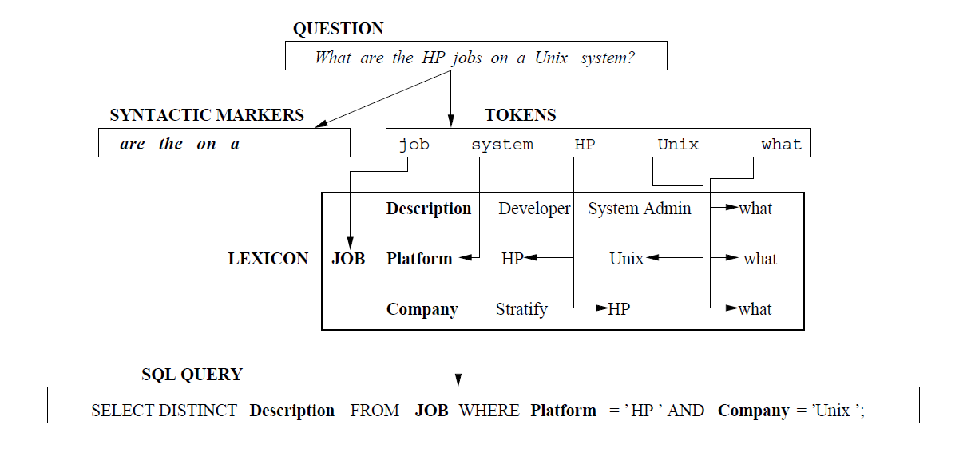
\includegraphics[scale=1.0]{graficos/popescu-example}
    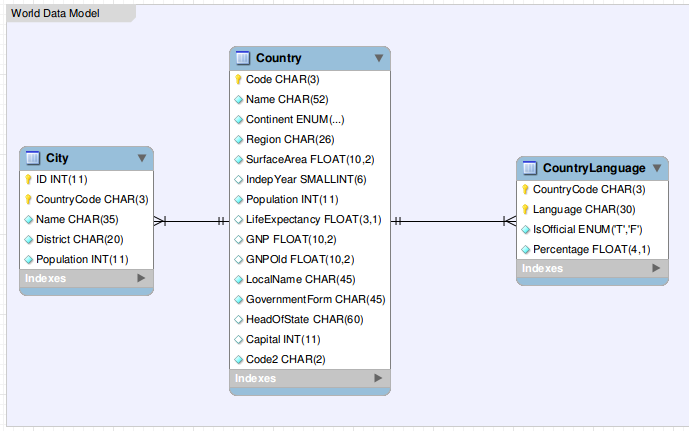
\includegraphics[width=12.823cm,height=8.004cm]{graficos/fuentes/world-db.png}
  \caption{Modelo entidad relación de la base de datos World original}
  \label{fig:world-db}
\end{figure}

La tabla Country tiene información básica acerca de varios países del mundo. La tabla City tiene información sobre las mayores ciudades del mundo y, finalmente, la tabla CountryLanguage tiene información sobre los idiomas hablados en cada país.

Hay una relación de uno a muchos entre Country y CountryLanguage: cada país puede tener más de un idioma y, además, hay una relación de uno a muchos entre Country y City: cada país puede tener más de una ciudad.

\medskip
Las definiciones de las relaciones originales son:
\begin{itemize}
\item Country(Code, Name, Continent, Region, SurfaceArea, IndepYear, Population, LifeExpectancy, GNP, GNPOld, LocalName, GovernmentForm, HeadOfState, Capital, Code2)
\item City(ID, ContryCode, Name, District, Population)
\item CountryLanguage(CountryCode, Language, IsOfficial, Percentage)
\end{itemize}


Para nuestro proyecto, renombramos algunos de los elementos:
\begin{itemize}
\item La relación CountryLanguage fue renombrada a Language
\item El atributo Language de la relación CountryLanguage fue renombrado a Name
\item El atributo IndepYear de la relación Country fue renombrado a IndependenceYear
\end{itemize}

En las tablas X, Y, Z pueden verse algunas filas de ejemplo de cada una de las tablas y, en la tabla W, el total de filas de cada una.
%TODO: HACER TABLAS!!!

Incorporando estos datos al modelo teórico, hasta aquí tenemos definidos: la base de datos, sus elementos ($E$) y el tipo de sus elementos.


\section{Implementación}
\label{sec:popescu-implementacion}

El código de la implementación está disponible en github: acá. Está implementado en java e implementa, con la mayor fidelidad posible, el sistema propuesto por Popescu y descripto en \allref{subsec:closed-domain}.
%TODO: acá

Estructuramos esta sección como sigue. Primero (\ref{subsec:popescu-codigo}), discutimos la implementación en sí misma, analizando los módulos más importantes del sistema  (Fill me, Neddy!), luego (\ref{subsec:popescu-ejemplos}) mostramos y comentamos algunos ejemplos de ejecuciones y, finalmente ((\ref{subsec:popescu-cierre})), analizamos analizamos alcances, límites y trabajo futuro.
%TODO: completar las referencias a subsubsections

\subsection{Código}
\label{subsec:popescu-codigo}

Estructura general y librerías usadas y principales módulos
Lexicon: (wordnet + edu.mit.jwi)
%TODO: Hace intro de código

\subsubsection*{Lexicón}
\label{subsubsec:lexicon}
El lexicón, recordemos, es el módulo encargado de generar un conjunto de tokens para cada  elemento de la base de datos. Una vez construido este conjunto, las responsabilidades del módulo son las siguientes:
\begin{itemize}
	\item Dado un lema, devolver el conjunto de tokens que lo contienen
	\item Dado un token, devolver el conjunto de elementos de la base de datos que le \textit{corresponden}.
\end{itemize}

El lexicón está implementado en la clase $uba.modules.Lexicon$. Debemos distinguir los momentos de construcción y de consulta del mismo. La construcción, cuyo punto de entrada es el módulo $uba.app.CreateLexicon$, ocurre por separado, y debe ejecutarse una vez antes de poder utilizar el sistema para responder preguntas. Esta genera 4 archivos con formato json, que son luego cargados en memoria al momento de realizar consultas.

En el centro la construcción del lexicón se encuentra Wordnet (una base de datos léxica en inglés, que consta de conjuntos de sinónimos, definiciones de los mismos y relaciones semánticas entre ellos). Utilizamos esta base de datos para obtener los sinónimos de los elementos de la base de datos.

El input del algoritmo es la lista de los elementos de la base de datos (relaciones, atributos y valores) como strings. El primer paso es eliminar el camel case y separar y lematizar las palabras (la tokenizamos en el sentido dado por Popescu a token). Por ejemplo, después de este paso, el elemento GovernmentForm se convierte en el token \{government, form\}. En este paso eliminamos también las stopwords (por ejemplo, HeadOfState se convierte en \{head, state\}).

Luego, los datos paran por el TokenAugmenter, que simplemente agrega algunos sinónimos escritos a mano a algunos de estos elementos. Por ejemplo, para el elemento region (atributo de la relación country), agregamos el término location, para el elemento surface area agregamos los términos total size y square kilometers. Este paso es llevado a cabo por la clase uba.db.TokenAugmenter y su intención es mejorar las chances de obtener sinónimos útiles a partir de wordnet, ampliando su input de trabajo. Al salir del TokenAugmenter tenemos, para cada elemento de la base de datos, un conjunto (que puede tener un solo string si el TokenAugmenter no tenía ningún sinónimo) de tokens (que son, a su vez, listas de lemas).

%TODO: tal vez, agregar tabla de TokenAugmenter.

El tercer paso es el central: en este se obtienen, para cada uno de estos tokens, tokens sinónimos. Para esto obtenemos una lista de sinónimos y palabras relacionadas para cada lema del token, luego los combinamos formando todos los sinónimos ordenados. Por ejemplo, si el token original consistía de los lemas (A, B) y para A obtuvimos los sinónimos \{A1, A2\} y para B los sinónimos \{B1 y B2\}, el resultado serán todas las combinaciones ordenadas posibles: \{(A, B), (A, B1), (A, B2), (A1, B), (A1, B1), (A1, B2), (A2, B), (A2, B1), (A2, B2)\}.

Finalmente, intentamos obtener sinónimos también de todas las palabras del token juntas (incluyendo las stopwords), ya que verificamos empíricamente que para algunas de ellas existía una entrada en wordnet (Por ejemplo head of state produce el sinónimo chief of state que se pierde sin este paso).

El conjunto de tokens sinónimos para cada elementos de la base de datos es luego invertido, es decir, en lugar de disponer de un mapeo de elementos de la base de datos a conjunto de tokens sinónimos, construimos un mapeo de tokens en elementos de la base de datos.

Vale mencionar que en este índice invertido agregamos también tokens para cada qword posible, mapeando a un solo elemento especial, de tipado similar a un valor (WhValue), mediante el cual los tokens de qwords acceden al espacio de elementos de la base de datos. Además, para estos WhValues definimos a mano la relación de compatibilidad con atributos de la base de datos tal como se define en los papers. Esta relación está definida en la clase $uba.db.WhGenerator$ tal como la presentamos en la tabla \ref{table:atributos-qwords}.

\begin{center}
\begin{table}[h]
\centering
\begin{tabular}{| l |  p{12cm} |}
\hline
Qword & Atributos relacionados \\ \hline
What & Name, District, Population, Code, Continent, SurfaceArea, LifeExpectancy, GNP, LocalName, GovernmentForm,
                         Capital, IsOfficial, Percentage, Region \\ \hline
Which & Los mismos que para what\\ \hline
Where & Region, Continent, Capital, District\\ \hline
Who & HeadOfState\\ \hline
When & IndependenceYear\\ \hline
\end{tabular}
\caption{Atributos compatibles con cada Qword}
\label{table:atributos-qwords}
\end{table}
\end{center}

A partir de este mapeo son generadas algunas estructuras utilizadas para optimizar la performance del sistema, pero sin valor teórico (por ejemplo, la lista de todos los tokens, que es también el conjunto de índices del índice invertido). Estos datos son finalmente grabados en 4 archivos, que son luego cargados a memoria en el sistema principal.

Desde la perspectiva de la lectura, las operaciones son triviales. La interfaz de servicios ofrece los métodos getTokens() y getMatchingElements(). getTokens() es la encargada de devolver, para un lema, el conjunto de tokens que lo contienen, mientras que getMatchingElements() es la encargada de devolver, dado un token, el conjunto de elementos de la base de datos que le corresponden.

Discutamos ahora la implementación del tercer paso, en el que se obtienen sinónimos y palabras relacionadas para cada lema y luego se combinan.

En el caso ideal, lo que se busca es lograr un conjunto de sinónimos para una serie de palabras. Pero lo que entendemos por conjunto de sinónimos se ve opacado por un fenómeno lingüístico conocido como polisemia que es, en algún sentido, un fenómeno inverso a la sinonímia. Al utilizar wordnet siempre existe este problema. La polisemia refiere al hecho de que una palabra puede tener más de un sentido. Es el caso de la palabra banco, que puede ser tanto un asiento en una plaza como una institución financiera. La polisemia es un fenómeno que ocurre en el espacio de relaciones entre las palabras y los conceptos, al igual que la sinonímia, que refiere al hecho de que diferentes palabras pueden referir al mismo concepto (inodoro y retrete). En el core de wordnet existe el tipo de dato synset (conjunto de sinónimos, a veces traducido como anillo de sinónimos), en el que se agrupan, bajo un sentido o concepto, todas las palabras que lo refieren.

En general, los humanos podemos distinguir qué sentido de una palabra polisémica está en uso por contexto. Entre nuestras funciones cognitivas está el reconocer que si alguien dice voy a hacer un depósito al banco, nosotros entendamos que banco, en este contexto, refiere a la institución financiera y no al asiento de plaza. Pero sin contexto es imposible saber de qué sentido se está hablando.

Este problema no es tematizado en los trabajos de Popescu y, sin embargo, ellos argumentan que el sistema Precise fue construido con wordnet sin ningún tipo de desambiguador contextual previo.
En realidad, existe un atenuante para este problema que es el contexto de uso y el rol que cumplen los conjuntos de sinónimos y es que el conjunto de todos los tokens sinónimos generados funciona como un filtro sobre consultas del usuario y nunca es activo o productivo.
Consideremos, por ejemplo, una base de datos sobre localización de sucursales de bancos y el elemento Banco (por ejemplo, el nombre de una relación).
Buscando en sinonimos.com obtenemos los siguientes sinónimos, separados en dos líneas: 1) entidad crediticia, 2) taburete, escabel, escaño, peana, sitial, asiento. Tomando todos los sinónimos tendríamos el siguiente conjunto de sinónimos: {banco, (entidad, crediticia), taburete, escaño, peana, sitial, asiento} donde hay, mezclados, dos sentidos. Ahora bien: ¿qué uso hacemos de este conjunto? El usuario de una aplicación sobre localización de bancos introduce una pregunta, el sistema la separa, lematiza y chequea si los lemas pertenecen a algún conjunto de sinónimos. En este contexto, ¿es un problema que tengamos en término asiento en nuestro conjunto de sinónimos? Sería un problema solo si el usuario pudiese introducirlo, ya que al conjunto de sinónimos solo se accede a partir de palabras introducidas por el usuario. Si bien este problema es posible, no es probable y, quizás, siguiendo este razonamiento, quienes propusieron el modelo no hicieron ningún énfasis en este problema.

Nuestro sistema no introduce ningún desambiguador de sentido: utilizamos todo los sinónimos disponibles de tipo sustantivo, introduciendo potenciales errores de interpretación en este punto, con la salvedad recién mencionada.


Finalmente, agregamos también derivaciones léxicas lematizadas. Una derivación léxica es una variación de la palabra original que da otro sentido (relacionado) a la palabra original. Por ejemplo: existir, existencia, existencial, existiendo, existente son una serie de variaciones de la misma raíz.  Esta opción es experimental y puede activarse o desactivarse desde el archivo de configuración (uba.app.Config)

En la tabla \ref{table:sinonimos} pueden verse algunos ejemplos de los resultados.

\begin{center}
\begin{table}[h]
\centering
\begin{tabular}{| l |  p{9.5cm} | p{4cm} |} \hline
Lema & Sinónimos & Derivaciones léxicas\\ \hline
city 	&	metropolis, (urban, center)	&	citify, metropolitan\\ \hline
country	&	state, nation, land, commonwealth, (res, publica), (body, politic), (rural, area), area	&	--\\ \hline
language	&	language, linguistic communication, speech, speech communication, spoken communication, spoken language, voice communication, oral communication, lyric, words, linguistic process, terminology, nomenclature & lyricist, lyric, speak, terminological \\ \hline
region	&	region, part, area, neighborhood, realm	&	--\\ \hline
location	&	location, placement, locating, position, positioning, emplacement, localization, localisation, fix	&	locate, position, posit, emplace, localize, localise\\ \hline
continent	&	--	&	continental\\ \hline
gnp	&	gross national product	&	--\\ \hline
government	&	government, authorities, regime, governing, governance, government activity, administration, politics, political science	&	govern, political scientist\\ \hline
form	&	form, word form, signifier, descriptor, kind, sort, variety, shape, pattern, configuration, contour, conformation, human body, physical body, material body, soma, build, figure, physique, anatomy, bod, chassis, frame, flesh, cast, variant, strain, var., phase, class, grade, course, mannequin, manikin, mannikin, manakin	&	signify, sort, form, shape, pattern, contour, anatomic, anatomist, anatomical, shapely, variant\\ \hline
\end{tabular}
\caption{Lemas, sinónimos y derivaciones léxicas}
\label{table:sinonimos}
\end{table}
\end{center}

\subsubsection*{Tokenizer}
\label{subsubsec:tokenizer}

El Tokenizer en el modelo de Popescu, recordemos, es el encargado de generar todas las tokenizaciones completas de la pregunta y, para cada token, consultar al Lexicon y retornar la lista de elementos de la base de datos que le corresponden.

\medskip

El Tokenizer sigue el siguiente procedimiento:
\begin{enumerate}
\item Separar la pregunta en palabras, eliminar puntuaciones y pasar a lower case.
\item Lematizar las palabras. Para esto usamos Freeling
\item Eliminar marcadores sintácticos.
\item Para cada lema, obtener todos los tokens que lo contienen del Lexicon (método getTokens).
\item Para cada token potencial (resultado del paso anterior) verificar que todos sus lemas están presentes en el conjunto de lemas de la pregunta original.
\item Generar el conjunto de partes de todos los tokens hasta aquí obtenidos\footnote{El conjunto de partes de un conjunto dado es otro conjunto formado por todos los subconjuntos del mismo. Por ejemplo, el conjunto de partes de A = \{1, 2, 3\} es: \{ $\varnothing$, \{1\}, \{2\}, \{3\}, \{1, 2\}, \{2, 3\}, \{1, 3\}, \{1, 2, 3\} \}}. \\ \\
	Probando con cada elemento del conjunto de partes en lugar de utilizar solamente el conjunto original podemos obtener subconjuntos que cumplan también la condiciones requeridas para considerarse una tokenización completa (evaluados en 7).
\item Para cada uno de estos subconjuntos, verificar 1) que sus tokens cubran completamente los lemas significativos de la pregunta original y 2) que no haya stems repetidos entre los tokens.
\end{enumerate}

El resultado será un conjunto de tokenizaciones completas. Como se ve, respetamos casi al pie de la letra la implementación sugerida por Popescu. La obtención de los elementos de la base de datos que corresponden a los elementos, por una cuestión implementativa, quedó en manos del Matcher y no del Tokenizer. La implementación, de todos modos, del servicio, está en el Lexicon. Con este conjunto de tokenizaciones completas como input, será responsabilidad del Matcher decidir cuáles de ellas son traducciones válidas.

\subsubsection*{Matcher}
\label{subsubsec:matcher}

El Matcher, por su parte, toma las tokenizaciones completas generadas por Tokenizer y construye el grafo que expusimos con detalle en la sección \ref{subsec:closed-domain} y ejecuta el algoritmo de max flow. El problema de max-flow es un problema de grafos que consiste en “enviar” el máximo flujo posible a través de un grafo dirigido con dos nodos especiales (fuente o source y sumidero o sink) y aristas con cierta capacidad mayor o igual que cero. Este flujo debe ir desde el nodo fuente al nodo sumidero, respetando las capacidades de las aristas y respetando que, para cada nodo, el flujo saliente no puede ser mayor al flujo entrante.

Existen diferentes algoritmos para resolver este problema. En nuestra implementación, tomamos un código libre disponible en internet (aquí: \url{http://web.mit.edu/~ecprice/acm/acm08/MaxFlow.java}).

Las aristas implicadas en el flujo máximo posible asocian 1) los tokens de valor y de atributo y los correspondientes elementos (valores y atributos, respectivamente) de la base de datos y 2) pares de valores y atributos entre sí.

Después de esto, buscamos otras soluciones posibles de máximo flujo, dado que cualquier solución que tenga como valor para el máximo flujo la cantidad de tokens de valor en la pregunta es, potencialmente, una traducción válida. Para hacer esto retiramos, ordenadamente, las aristas del grafo que ocurren entre la columna 2 y 3 (tokens de valor y valores de la db).

Cabe notarse aquí, como ya mencionamos anteriormente, que no soportamos en nuestra implementación la desambiguación de tokens de relación. Esto significa que: asumimos que un token de relación tiene un solo elemento relación asociado y no será necesario decidir si refiere a una relación u a otra. En todos los ejemplos de bases de datos que consideramos, esta asunción era verdadera (es decir, no existía un token de relación que necesite ser desambiguado) y por ello no implementamos esta capacidad del sistema, que quedará como trabajo futuro.

\medskip

Finalmente, verificamos cuales de las soluciones con máximo flujo cumplen las condiciones requeridas para ser una traducción válida según enunciamos en \ref{subsec:closed-domain}:

\begin{enumerate}
\item Todos  los tokens de la tokenización tienen un único elemento de la base de datos asociado y no hay elementos de la base de datos repetidos. (Mapping.meetsConditionOne())
\item Cada token de atributo se relaciona con un único token de valor respetando que: (Mapping.meetsConditionTwo))
\begin{enumerate}
\item el atributo relacionado con el token de atributo y el valor relacionado con el token de valor son compatibles (esta condición está garantizada por el max-flow mismo)
\item ambos tokens están sintácticamente asociados
\end{enumerate}
\item Cada token de relación está relacionado a un token de atributo o bien a un token de valor, cumpliendo las siguientes condiciones: (Mapping.meetsConditionThree())
\begin{enumerate}
\item	la relación de la base de datos que corresponde al token de relación y el elemento de la base de datos que corresponde al token de atributo o token de valor son compatibles
\item ambos tokens (token de relación - token de atributo o bien token de relación - token de valor) están sintácticamente asociados
\end{enumerate}
\item La pregunta tiene una qword (Mapping.oneWhValue())
\end{enumerate}

Notemos que la condición 3 implica que para cada token de relación exista algún token de atributo o de valor a) compatible y b) sintácticamente asociado. La condición a) no está verificada por el algoritmo de máximo flujo y es verificada en el método Mapping.valid()

Para verificar las condiciones de asociación sintáctica (2.b y 3.b) utilizamos la implementación oficial del árbol sintáctico de Charniak (\url{github.com/BLLIP/bllip-parser}), con un wrapper en java que es la clase uba.nlp.CharniakParseTree. Las reglas sintácticas utilizadas por los creadores del modelo no están especificadas en sus trabajos, por lo que creamos nuestras propias reglas tomando los ejemplos de asociaciones sintácticas dadas en los trabajos, evaluando los resultados de diferentes ejemplos y extrapolando reglas a partir de allí.


Veamos, en primer lugar, algunos ejemplos del parse tree:

``What are the HP jobs on a Unix system?''

(S1 (SBARQ (WHNP (WP What)) (SQ (VP (AUX are) (NP (DT the) (NNP HP) (NNS jobs)) (PP (IN on) (NP (DT a) (NNP Unix) (NN system))))) (. ?)))

``What are the capitals of the US states?''
(S1 (SBARQ (WHNP (WP What)) (SQ (VP (AUX are) (NP (NP (DT the) (NNS capitals)) (PP (IN of) (NP (DT the) (NNP US) (NNS states)))))) (. ?)))


``What are the names of cities of Argentina?''
(S1 (SBARQ (WHNP (WP What)) (SQ (VP (AUX are) (NP (NP (DT the) (NNS names)) (PP (IN of) (NP (NP (NNS cities)) (PP (IN of) (NP (NNP Argentina)))))))) (. ?)))

En las figuras \ref{fig:word-tags} y \ref{fig:syntax-tags} pueden verse los diferentes tags para hojas y para nodos intermedios (respectivamente).


\begin{figure}[H]
  \centering
    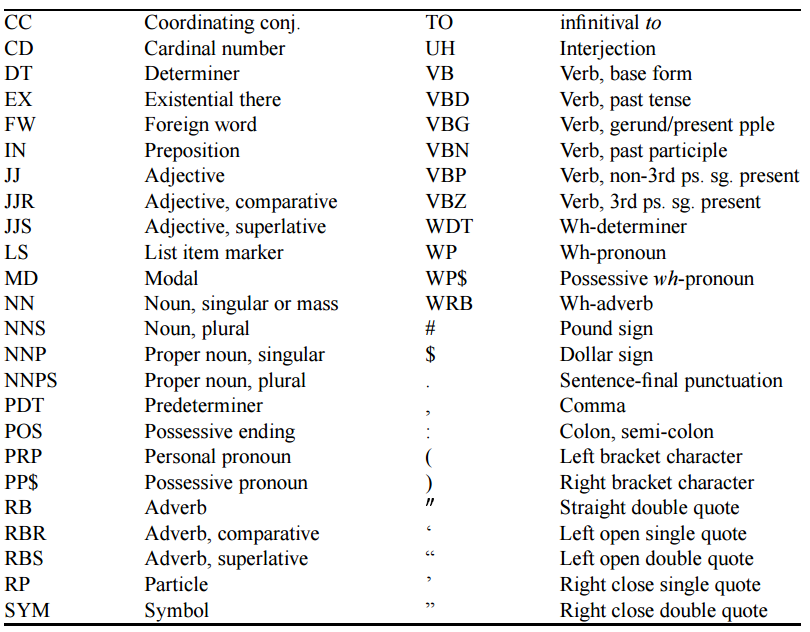
\includegraphics[width=12.823cm,height=8.004cm]{graficos/fuentes/WordTags.png}
  \caption{POS tags de Penn Treebank}
  \label{fig:word-tags}
\end{figure}


\begin{figure}[H]
  \centering
    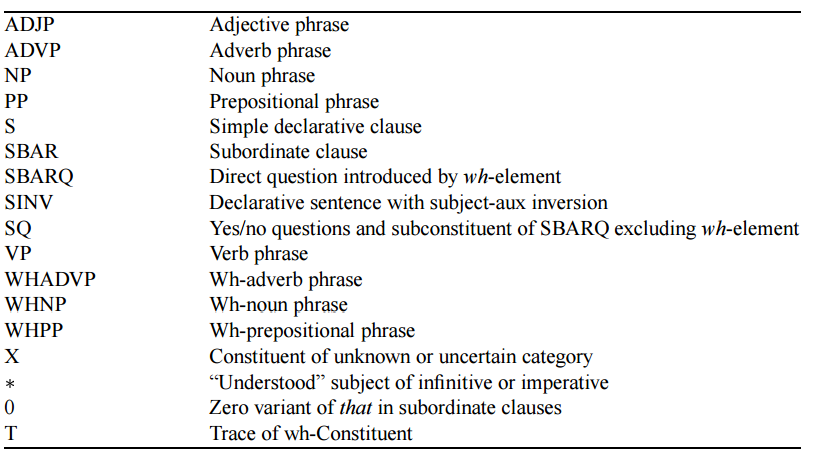
\includegraphics[width=12.823cm,height=8.004cm]{graficos/fuentes/SyntaxTags.png}
  \caption{Conjunto de tags para nodos intermedios del árbol sintáctico}
  \label{fig:syntax-tags}
\end{figure}



Las reglas que construimos son las siguientes. Notar que presentamos flechas unidireccionales (y los nombres dados indican lo mismo) pero las relaciones son simétricas.

\begin{enumerate}
\item Hermanos: NNx <==> NNx <==> Wx si tienen el mismo padre
\item Qwords a sustantivo:
a.	Una Wx dentro de un WHNP ==> un NNx dentro de un NP dentro de un VP dentro de un SQ
\item Sintagma nominal a sintagma preposicional:
a.	NNx dentro de un NP ==> NNx dentro de un NP dentro de un PP del mismo padre que el NP original
\item Sintagma nominal a sintagma verbal
a.	NNx dentro de un NP ==> NNx dentro de un NP dentro de un VP del mismo padre que el NP original
\end{enumerate}

La definición de las reglas se hizo a prueba y error y es posible que sea simple, para alguien con mayores conocimientos lingüísticos, mejorarlas. El sistema ofrece también la opción de no evaluar las asociaciones sintácticas en absoluto ($Config.DO_NOT_CHECK_CHARNIAK$), en cuyo caso se mejora la performance pero aparecen nuevas traducciones válidas que podrían haber sido filtradas por estas condiciones, que el usuario deberá desambiguar manualmente).

Finalmente, todos los resultados de max-flow que cumplen con las condiciones de 1 a  4 son traducciones válidas, que pasan al MappingFilter, que realiza ciertos filtrados que describiremos, de nuevo, en un título aparte.

El resultado de este módulo es una lista de Mappings (una estructura que contiene 1) una tokenización completa de la pregunta original y 2) un mapeo válido entre cada token de la misma en un elemento de la base de datos). Cada mapeo es una traducción válida de la pregunta. Si existe solo uno, entonces este mapeo se traducirá en una query que generará el resultado. Si no, corresponde al MappingFilter realizar filtrados inteligentes de las múltiples soluciones y, en caso de que continuen existiendo múltiples soluciones, entonces se consultará al usuario qué quiso preguntar. Por otro lado, si no fue posible generar ninguna traducción válida, se retornará al usuario sin respuesta, pidiéndole que vuelva a escribir su pregunta de otro modo.


\subsubsection*{MappingFilter}
\label{subsubsec:mapping-filter}

La clase uba.app.MappingFilter contiene una serie de reglas para filtrar traducciones válidas que utilizamos de manera experimental, de las cuales solo conservamos la eliminación de traducciones repetidas. Para eliminar las traducciones repetidas, las transformamos en queries y simplemente comparamos por igualdad, ya que el generador de queries ordena las cláusulas generando, para inputs iguales pero diferentemente ordenados, la misma query.

%TODO: La regla del preferred implicit.


\subsubsection*{QueryGenerator}
\label{subsubsec:query-generator}

El procedimiento para generar una query a partir de una traducción válida es exactamente el mismo que se desarrollo en \ref{subsec:closed-domain} y está implementado en el método Mapping.query().


\subsubsection*{MainProcessor}
\label{subsubsec:main-processor}

Finalmente, el punto de entrada de todo el sistema es uba.app.MainProcessor, que puede utilizarse especificando el parámetro -q QUESTION en cuyo caso responderá a esa pregunta y retornará el control o bien sin parámetros, en cuyo caso ingresa en un loop de preguntas-respuestas. El resultado para cada pregunta es cero, una o más queries de SQL.
Agregamos la opción de desambiguación para que el usuario elija entre dos o más queries si no se pudo generar una y también una presentación de las respuestas una vez determinada la query final, pero es más bien experimental y poco sólido.



\subsection{Ejemplos}
\label{subsec:popescu-ejemplos}


\subsection{Limitaciones y Trabajo Futuro}
\label{subsec:popescu-cierre}
\chapter{Implementación sobre Qanus}
\label{chap:qanus}
\cerradaarg{Sin supervisar}
En este capitulo veremos la implementación del modelo de question answering multilingüe y diferentes evaluaciones realizadas utilizando como guia dos tareas monolingües de la competencia QA@Clef '07, una para español y otra para portugués. El sistema está basado en un framework académico de código abierto llamado Qanus. Este framework está empaquetado con una sistema de QA simple, QA-sys, que resuelve ejercicios de la competencia Trec '07 con soporte para inglés. Nosotros adaptamos este sistema para utilizar como librería de procesamiento de lenguajes a Freeling, generando un sistema baseline multilingüe. A este sistema le agregamos features reseñados en \allref{sec:literatura} y realizamos diferente mediciones sobre las instancias en español y portugués sobre los ya mencionados ejercicios de Clef '07.

La estructura de este capitulo es la siguiente: en \allref{sec:ejecicio-de-clef} se describe con detalle el panorama general de tareas de question answering en la competencia Clef '07, haciendo énfasis en las tareas seleccionadas, en los corpus y las preguntas disponibles y en las decisiones tomadas a la hora de elegir estas tareas; en \allref{sec:sistema} se comenta la adaptación del sistema baseline y las modificaciones realizadas a los algoritmos, {\color{red}mientras que los resultados pueden observarse como apartados en las mismas secciones o como una sección aparte al final}.

\section{Ejercicio de Clef}
\label{sec:ejecicio-de-clef}
\cerradaarg{Sin supervisar}
Tras investigar distintas competencias y métodos de evaluación, optamos por utilizar como guía de trabajo dos ejercicios de la tarea principal de question answering de la competencia Clef de 2007. Principalmente por contar con un subconjunto de ejercicios bastante adecuados para nuestra tesis y disponer de un corpus de datos libre y disponible en el acto para evaluar una parte importante de las funcionalidades implementadas en nuestro proyecto. 

Como mencionamos en \allref{sec:competencias}, Clef (de \textit{Cross-Language Evaluation Forum}) es una organización que busca fomentar la investigación en sistemas de information retrieval cross-language. En particular, una vez por año Clef lanza una competencia de Question Answering multilingüe, con diferentes corpus y diferentes tipos de ejercicios. Estas competencia permiten obtener un patrón estándar de comparación entre distintos desarrollos y una idea general del estado de arte alcanzado en los diferentes idiomas por la diferentes actores académicos o {\color{red}comerciales}. Por lo demás, Clef es el principal organizador de conferencias de question answering multilingüe para idiomas europeos y la tarea principal de '07 presentaba una complejidad adecuada para el scope de esta tesis.

La competencia de 2007 es la quinta campaña de QA multilingüe de Clef, siendo la primera en 2003 {\color{red} tomando la posta dejada por las Trec multilingües}. 

La tarea estandar principal de question answering incorpora algunas particularidades que la diferencian de anteriores campañas: los temas o tópicos, la co-referencia y el uso de wikipedia como corpus de datos parcial. Además de la tarea principal se presentaron tres tareas más: Answer Validation Exercise (AVE) y QUAST, question answering in speech transcription y Question Answering Real Time, con métricas de performance temporales. Como nota general, es importante notar que las tareas fueron de una complejidad elevada y en comparación con los resultados del año anterior, la mejor precisión general bajó del 49\% al 41.75\% para tareas multi-lingües, mientras que, más significativamente, bajó de 68\% a 54\% en tareas monolingües.


\subsection{Tareas}
\label{subsec:tareas}
\cerradaarg{Sin supervisar}
Utilizamos como guia dos ejercicios de la tarea principal de question answering de '07  por varias razones (Ver \cite{GuidelineClef07} y \cite{OverviewClef07} para un detalle exhaustivo de la conferencia en cuestión). Para esta tarea estaban disponibles en acto corpus, inputs de prueba y resultados esperados para una experimentación multilingüe que abarque tanto inglés como español y portugués. Además, estos ejercicios incorporaban, por única vez, diferentes wikipedias como parte del corpus de datos, lo cual resulta de por si atractivo. 

La tarea principal de QA de Clef '07 ofrece dos grandes grupos de ejercicios:
\begin{itemize}
\item Mono-lingual: donde el idioma de la pregunta y el idioma de la fuente de información son el mismo
\item Cross-lingual: donde el idioma de la pregunta y el idioma de la fuente de información difieren
\end{itemize}

En ambos grupos, los sistemas reciben un set de 200 preguntas - que pueden ser de hechos o eventos (FACTOID), definiciones de personas, cosas u organizaciones (DEFINITION), listas de personas, objetos o datos (LIST) - y se exige devolver una respuesta exacta, donde exacta significa sin más información de la mínima necesaria. Siguiendo el ejemplo de Trec, los ejercicios de este año contienen topics, i.e. clusters de preguntas relacionadas con un mismo tema y con posibilidad de co-referencia entre las preguntas del grupo. Ni el tipo de la pregunta ni el tópico es dado a los participantes.

La respuesta tiene que estar soportada por el id del documento del cual se extrajo y por la porción de texto que proveyó contexto suficiente para soportar la corrección de la respuesta. Los “textos de soporte” pueden venir de diferentes partes de documentos relevantes y deben sumar un máximo de 700 bytes. No hubo restricciones sobre la longitud del string de respuesta, pero fragmentos de información innecesaria fueron penalizados marcando la respuesta como ineXacta. 

Otra particularidad de los ejercicios es que hay preguntas sin respuesta en el corpus que esperan como respuesta 'Nil'.


Se consideraron 10 idiomas para preguntas: búlgaro, holandés, inglés, francés, alemán, indonesio, italiano, portugués, romano y español. Todos estos idiomas se usaron como idiomas del corpus, a excepción del indonesio para el que no se disponía de una colección de noticias.

Se propusieron, en total, 37 tareas concretas: 8 monolingües y 29 bilingües. Dada la complejidad de la construcción del ejercicio mismo, la organización solo implementó concretamente las tareas tomadas por algún equipo competidor. 


\begin{figure}
  \centering
    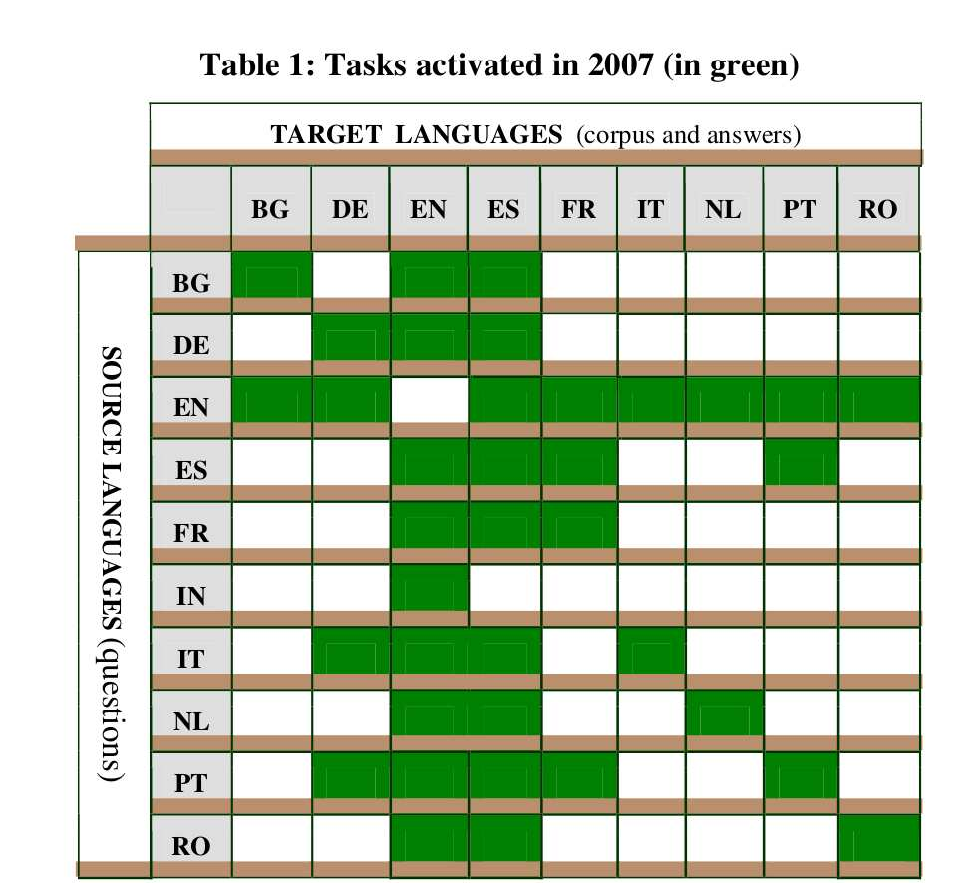
\includegraphics[scale=0.5]{graficos/clef07}
  \caption{Tareas activadas en la competencia Clef '07}
  \label{fig:tareas}
\end{figure}

El corpus de datos propuesto consiste en dos corpora distintos: una serie de de recopilados especificamente por los organizadores de la competencia y utilizado con frecuencia en competencias anteriores y, por otro lado, snapshops de las wikipedias en diferentes idiomas con límite en Diciembre de 2006.

Para nuestro proyecto utilizamos las preguntas y los datos de evaluación de los ejercicios monolingües es-es (español-español) y pt-pt (portugués-portugués) implementando como corpus de datos solo las wikipedias.

Los datos de los ejercicios constan de dos archivos: un archivo con 200 preguntas agrupadas por temas y otro archivo con diferentes traducciones de la pregunta, una respuesta goldstandard con soporte textual y el id del documento de soporte para el idioma target (del corpus). 

Por otro lado, en la guía de ingreso a la competencia\cite{GuidelineClef07} se proveen links para descargar los snapshots de wikipedia sugeridos. Se ofrece una versión de wikipedia en inglés preprocesada de Noviembre de 2006 \footnote{\url{http://ilps.science.uva.nl/WikiXML/}}, dos opciones para descargar wikipedia en español: una imagen estática en html de Noviembre de 2006 \footnote{\url{http://static.wikipedia.org/downloads/November_2006/es/}} y un dump xml de Diciembre de 2006 \footnote{\url{http://download.wikimedia.org/images/archive/eswiki/20061202/pages-articles.xml.bz2}} y también X opciones de portugués.

La guía aclara que, bajo responsabilidad de los participantes, se puede usar
cualquier otra versión de Wikipedia, siempre y cuando sea anterior a noviembre / diciembre de 2006.
Además, se pide que las respuestas sean tomadas de ``entradas reales" o artículos de wikipedia y
no de otros documentos (imagenes, discusión, categoría, template, histórico de reviosones, datos de usuario y páginas con meta información).

Los links a páginas de wikipedia en español y en portugués no estaban más disponibles (ambos respondieron 404), mientras que el formato
preprocesado pedido para el inglés resultaba realmente complejo de instalar y parecía una linea muerta. Por estos motivos,
seguimos la sugerencia sobre el uso responsable de otras wikipedias y utilizamos las siguientes snapshots de Wikidumps\footnote{Ver \url{http://dumps.wikimedia.org/} y \url{http://en.wikipedia.org/wiki/Wikipedia:Database_download\#Other_languages}}.

\begin{center}
\begin{tabular}{ | l | l | l | l |}
    \hline
    Idioma & Fecha & Tamaño & \# Entradas \\ \hline
    Español & 5 de Julio de 2006 & 558M  & 233750  \\ \hline
    Portugués & 1 de Febrero de 2007 & 776M  & 498039  \\ \hline
    Inglés Simple & 4 de Julio de 2006 & 26M   & 18273   \\ \hline
    Inglés & 4 de Noviembre de 2006 & 7,6G  &   \\ \hline
    Español & 26 de Enero de 2007 & 902M  &   \\ \hline
    Español & 14 de Junio de 2013 & 7,3G  &   \\ \hline
    Inglés Simple & 24 de Julio de 2013 & 406M  &   \\ \hline
\end{tabular}  
\end{center}

Utilizando la información disponible en los archivos de respuestas esperadas, discriminamos las preguntas con respuestas con soporte de wikipedia, las soportadas por el corpora de noticias de la organización y las que no tienen respuesta (NIL):

\begin{center}
\begin{tabular}{| l | l | l | l | l |}
\hline
Idioma & Wiki & News & NIL & Total \\ \hline
es & 155 & 37 & 8 & 200 \\ \hline
pt & 130 & 59 & 11 & 200 \\ \hline
\end{tabular}
\end{center}


\subsection{Análisis de las preguntas}
\cerradaarg{Sin supervisar}
Las 200 preguntas del test set están agrupadas por tema, y cada tema tiene de una a cuatro preguntas. Los temas pueden ser entidades nombradas, evento o también categorías como objetos, fenómenos naturales, etc (por ejemplo: Bush, Juegos Olímpicos, notebooks, huracanes, etc). 
Los temas no están dados en el set de test, pero pueden ser inferidos del primer par pregunta respuesta. La relación del tema con el grupo de preguntas respetaba las siguiente condiciones:

\begin{itemize}
\item El tema es nombrado en la primer pregunta o bien en la primera respuesta.
\item Las siguientes preguntas pueden contener co-referencias al tema expresado en el primer par pregunta/respuesta
\end{itemize}


Para ilustrar el punto consideremos el primer grupo de preguntas para el ejercicio de español es:
\begin{itemize}
\item ¿En qué colegio estudia Harry Potter?
\item ¿Cuál es el lema del colegio?
\item ¿En qué casas está dividido?
\item ¿Quién es el director del colegio?
\end{itemize}


{\color{red} El set de preguntas estaba numerado de 1 a 200, sin indicación de si pertenecian a un cluster del mismo tema o no} 

Como ya mencionamos, algunas preguntas podían no tener respuesta en la colección de documentos, y en ese caso la respuesta exacta era “NIL” y la justificación y el docid vacíos. La organización definió como criterio de inexistencia de la respuesta que ni los asesores humanos ni los demás sistemas participantes pudieran encontrar alguna.

En lo que respecta a los tipos de pregunta, el ejercicio considerara tres categorías: Factoid, Definition y Closed List.

\begin{center}
\begin{table}
\begin{tabular}{| l |  p {12cm} |}
\hline
Tipo & Descripción  \\ \hline
FACTOID & preguntas fácticas, preguntando el nombre de una persona, un lugar, la medida de algo, el día en que algo ocurrió, etc. \\ \hline
DEFINITION & preguntas como Qué/ Quién es X? \\ \hline
CLOSED LIST & questions that require one answer containing a determined number of items, e.g \\ \hline
\end{tabular}
\caption{Definición de los tipos de pregunta}
\label{table:question-type-definition}
\end{table}
\end{center}

Todos los tipos de pregunta podian contener restricciones temporales, i. e: una especificación temporal proveyendo importante información para devolver una respuesta correcta. Por ejemplo: \newline
Q: Who was the Chancellor of Germany from 1974 to 1982? \newline
A: Helmut Schmidt.\newline
Q: Which book was published by George Orwell in 1945?\newline
A: Animal Farm.\newline
Q: Which organization did Shimon Perez chair after Isaac Rabin’s death?\newline
A: Labour Party Central Committee.\newline


%Los calculos propios coinciden con el análisis presentado en \cite{OverviewClef07} en la siguiente discriminación del total de preguntas en función de las categorías recién señaladas:
\begin{center}
\begin{table}
\begin{tabular}{| l | l | l | l | l | l |}
\hline
Subset & Idioma & Factoid & Definition & List & Total \\ \hline
\multirow{2}{*}{Todo} & es & 158 & 32 & 10 & 200 \\ \cline{2-6}
 & pt & 159 & 31 & 10 & 200 \\ \hline
 \multirow{2}{*}{Wiki} & es & 122 & 24 & 9 & 155 \\ \cline{2-6}
 & pt & 104 & 18 & 8 & 130 \\ \hline
\end{tabular}
\caption{Totales por tipo de pregunta}
\label{table:totals-type-question}
\end{table}
\end{center}

Los tipos de preguntas disponen a su vez de subtipos. Las preguntas factoid disponen de 8 subtipos, las de definiciones y listas tienen 4.
Se consideraron los siguiente 8 tipos de Factoids: 

\begin{center}
\begin{table}
\begin{tabular}{| l | p{12cm}|}
\hline
Tipo & Ejemplo \\ \hline
PERSON &  Q: Who was called the \dq{Iron-Chancellor}? \newline A: Otto von Bismarck. \\ \hline 
LOCATION & Q: Which town was Wolfgang Amadeus Mozart born in? \newline A: Salzburg. \\ \hline
ORGANIZATION & Q: What party does Tony Blair belong to? \newline A: Labour Party.\\ \hline
MEASURE &Q: How high is Kanchenjunga?\newline A: 8598m. \\ \hline
COUNT & Q: How many people died during the Terror of Pol Pot? \newline A: 1 million.\\ \hline
OBJECT & Q What does magma consist of?\newline A: Molten rock.\\ \hline
TIME & Q: What year was Martin Luther King murdered?\newline A: 1968.\\ \hline
OTHER & i.e. everything that does not fit into the other categories above.\newline Q: Which treaty was signed in 1979? \newline
A: Israel-Egyptian peace treaty.\\ \hline
\end{tabular}
\caption{Tipos de respuesta esperada para preguntas Factoid}
\label{table:type-factoid}
\end{table}
\end{center}

Las preguntas de tipo LIST consisten son enumeraciones de 4 tipos posibles: PERSON, LOCATION, ORGANIZATION y OTHER.
Por ejemplo:\newline
Q: Name all the airports in London, England. \newline
A: Gatwick, Stansted, Heathrow, Luton and City.

Como solo una fuente estaba estaba permitida, los items debían aparecer en secuencia, uno después del otro, en uno documento de la colección .
Con respecto a las preguntas de tipo definition, también cuatro tipos, con otra semántica.


\begin{center}
\begin{table}
\begin{tabular}{| l | p{12cm}|}
\hline
Tipo & Descripción y ejemplo \\ \hline
PERSON & i.e. questions asking for the role/job/important information about someone, \newline
 Q: Who is Robert Altmann? \newline
 A: Film maker. \\ \hline
ORGANIZATION & i.e. questions asking for the mission/full name/important information about an organization \newline
 Q: What is the Knesset? \newline
 A: Parliament of Israel. \\ \hline
OBJECT & i.e. questions asking for the description/function of objects, e.g. \newline
Q: What is Atlantis? \newline
A: Space Shuttle. \\ \hline
OTHER & i.e. question asking for the description of natural phenomena, technologies, legal procedures etc. \newline
Q: What is Eurovision? \newline
A: Song contest. \\ \hline
\end{tabular}
\caption{Tipos de respuesta esperada para preguntas Definition}
\label{table:definition-questions}
\end{table}
\end{center}

\begin{center}
\begin{table}
\begin{tabular}{| l | l | l | l | l | l |l |l|l|}
\hline
Tipo & pt & es & pt-factoid & es-factoid & pt-def & es-def & pt-list & es-list \\ \hline
COUNT & 21 & 22 & 21 & 22 & 0 & 0 & 0  & 0\\ \hline
OBJECT & 11 & 27 & 6  & 18 & 5 & 9 & 0  & 0\\ \hline
MEASURE & 15 & 20 & 15 & 20 & 0 & 0 & 0  & 0\\ \hline
PERSON & 33  & 35 & 21 & 24 & 9 & 8 & 3 & 3\\ \hline
TIME & 19 & 16 & 18 & 16 & 0 & 0 & 1 & 0\\ \hline
LOCATION & 33 & 18  & 30 & 18 & 0 & 0 & 3 & 0 \\ \hline
ORGANIZATION & 31 & 32 & 24 & 22 & 6 & 8 & 1 & 2\\ \hline
OTHER & 37 & 30 & 24 & 18 & 11 & 7 & 2 & 5 \\ \hline
Total & 200 & 200 & 159 & 158 & 31 & 32  & 10 & 10\\ \hline
\end{tabular}
\caption{Tipos de respuesta esperada en función de tipo de pregunta}
\label{table:tipo-general}
\end{table}
\end{center}


\section{Sistema}
\label{sec:sistema}
\cerradaarg{Sin supervisar}
Nuestra implementación está basada en Qanus como framework o arquitectura de diseño de QA y en Freeling como proveedor de servicios de procesamiento de lenguaje multilingue. Qanus (Question-Answering @ National University of Singapore) es un framework de question answering basado en information retrieval y también un sistema de QA funcional simple construido sobre este framework. El proyecto se actualizó por última vez en noviembre de 2012 y contiene herramientas actuales de nlp para inglés (el POS-tagger, el NER-tagger y el Question Classifier de Stanford) y también de information retrieval (índice de búsquedas lucene) bajo licencia de código abierto. El paquete cuenta con un framework (qanus), que cumple un rol equivalente a la arquitectura DeepQA en la organización del proyecto de IBM, y un sistema montado sobre este framework -QA-sys-, equivalente a Watson (Ver Figura ~\ref{fig:Quanus}). 

% La motivación del proyecto es proveer a la comunidad científica un framework para ingresar al mundo de QA de una manera más sencilla y rápida, permitiendo construir nuevos sistemas de QA sobre esta arquitectura. 

\begin{figure}
  \centering
    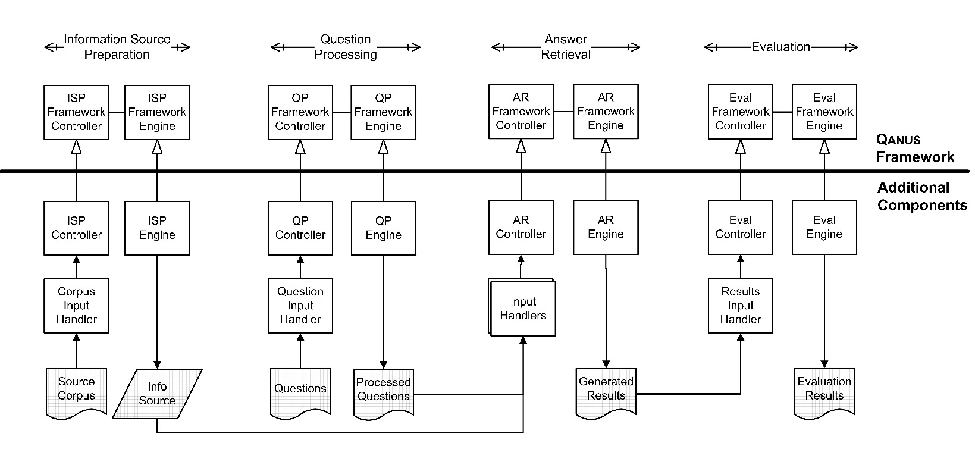
\includegraphics{graficos/Quanus}
  \caption{El framework Quanus y la implementación QA-sys}
  \label{fig:Quanus}
\end{figure}


La arquitectura de Qanus mantiene la estructura de pipeline típica similar a las reseñadas en la sección \allref{chap:estado-de-arte}. 
Consta de los siguientes pasos:

\textbf{Preparación de la fuente de información: } El primer step del pipeline es preprocesar las fuentes de información para un acceso optimizado en pasos posteriores del proceso. La implementación QA-sys incorpora una base de conocimiento en formato XML de AQUAINT\footnote{\ } a un índice de
búsquedas Lucene. En este paso se incorpora todo el conocimiento offline; bases de conocimiento dinámicas como la web se modelan en el pasos posteriores. \newline

\textbf{Análisis de la pregunta: } Este paso, igualmente genérico, permite la incorporación de
distintos componentes para anotar los tokens de la pregunta con datos
útiles para ser consumidos por el paso 3. Otro procesamiento a
realizar en este paso podría ser la generación de queries
entendibles por los distintos motores de almacenamientos de
información del paso 1. En particular, la implementación trae un
pos-tagger, un ner-tagger y un question classiffier, todos de Stanford.
Hablaremos más de estos componentes más adelante. \newline

\textbf{Generación de respuestas: } En este paso se utiliza la información generada en la preparación
de la base de información y en el procesamiento de la pregunta para
generar una respuesta. También puede incorporarse accesos a la web y
validaciones de las respuestas candidatas. La implementación concreta
evalúa cada pasaje de los primeros n documentos retornados por Lucene
para la pregunta original con una serie de componentes ad-hoc de
distancia para adjudicar diferentes grados de confiabilidad a los
distintos pasajes. \newline


Además, se provee de un cuarto paso opcional (el sistema de QA está
completo con los tres pasos anteriores), para la fase de desarrollo y
de evaluación de la performance del sistema:\newline


\textbf{Evaluación: }Este paso está pensado para evaluar las respuestas generadas y
presentarlas de un modo conciso en la fase de desarrollo.
Básicamente, cruza las respuestas obtenidas contra unas respuestas
esperadas escritas a mano y presenta el total de respuestas dadas
correctamente.\newline

En esta sección de la tesis adoptamos el framework Qanus y adaptamos el sistema QA-sys para 1) incorporar Freeling como librería de herramientas de procesamiento del lenguaje permitiendo un funcionamiento multilenguaje, 2) trabajar sobre el corpus de datos y preguntas de los ejercicios de CLEF '07 de español y portugués descriptos en \allref{sec:ejecicio-de-clef} y, finalmente, 3) incorporamos y evaluamos diferentes mejoras tomadas de la reseña a la literatura científica del apartado anterior \allref{sec:literatura}.

\subsection{Implementación de Qanus y QA-sys}
\cerradaarg{Sin supervisar}
El código está escrito en java y mantiene una interfaz común a
todos los pasos: un controller cuyas responsabilidades son cargar los
componentes y un engine que utiliza los componentes para leer el input,
procesarlo y grabar el resultado. La adaptabilidad del framework está
dada en la posibilidad de incorporar componentes respetando la interfaz
especificada para los mismos o bien, en modificar esta misma interfaz.

La implementación QA-sys está desarrollada para correr sobre
el tipo de datos de las evaluaciones Trec 2007. 
Brevemente, la implementación realiza las siguientes tareas:
En el primer paso, incorpora los XML en el formato XML Aquaint propuesto por la competencia a un índice Lucene, en
el segundo paso anota la pregunta con POS tags, NERs y
clasifica el tipo de respuesta con un clasificador entrenado y luego,
en el tercer paso se busca la pregunta sobre el índice lucene y se
retorna una lista con n documentos rankeados. Estos documentos se
subdividen en pasajes. Luego se aplican diferente algoritmos ad-hoc
dependiendo del tipo de respuesta esperada. \ Por ejemplo, si la
respuesta es un nombre de persona, se ejecuta NER sobre los diferentes
pasajes buscando nombres candidatos, si el tipo esperado es una fecha,
se utilizan expresiones regulares escritas a mano, etc. Finalmente, los
pasajes candidatos se evalúan utilizando heurísticas de proximidad
de los candidatos a la pregunta inicial. Para esto se utilizan
diferentes Scorers que rankean los pasajes según diferentes
características (features) y luego se selecciona alguna priorizando
algunas características sobre otras, dependiendo también del tipo
de respuesta esperada. Por último, el evaluador de resultados mide la
exactitud (\textit{accuracy}): total de respuestas correctas sobre
total de preguntas. 

QA-sys funciona sólo sobre preguntas del tipo
factoid y, a modo de comparación, el mejor sistema según la Trec
2007, el LymbaPA07 obtuvo un grado de exactitud del 0.706 y el décimo
(Quanta) obtuvo 0.206, mientras que QA-sys logra el 0.119 disponiendo de una implementación sumamente simple.

En las siguientes secciones de la tesis describiremos la implementación de nuestro sistema de question answering tomando como base los tres pasos principales del pipeline de QA-sys. 

\subsection{Base de conocimiento}
\cerradaarg{Sin supervisar}
El módulo de procesamiento de la base de información de la implementación QA-sys está desarrollada para correr sobre el tipo de datos de las evaluaciones Trec 2007, un formato XML conocido como ``Aquaint". Por otro lado, el mismo framework esta atado al procesador de XMLs SAX, una entre varias implementaciones disponibles en el entorno de java. En nuestra adaptación, incorporamos la librería gwtwiki\footnote{Java Wikipedia API (Bliki engine): \url{http://code.google.com/p/gwtwiki/}} para procesar los xml dumps de wikipedia. Como esta librería no utiliza SAX, nos vimos obligados a modificar el framework. 

En este proceso descartamos artículos mal formados y entradas representado imágenes o discusiones, tal como se sugiere en la guía. 
Los artículos se indexan en índices Lucene como documentos con los siguiente campos: \emph{id, title, body y all}. 
La tabla \ref{table:creacion-indices} muestra algunos datos del proceso de generación de índices, mientra que la figura \ref{fig:LuceneIndexWriterWiki} ilustra el proceso.

\begin{table}
\begin{center}
\begin{tabular}{| l | l | l | l | l | l| l|l|}
\hline
Wikipedia & \# Entradas & Nulas & Redirects & Filtradas & Validas & Tamaño & Tiempo \\ \hline
simple-06 & 18273 & 22 &  3452 & 5241 & 9558 & 26M & 14 secs \\ \hline 
es-06 & 233750 & 52 & 62805 & 34947 & 135946 & 558M & 242 secs\\ \hline 
pt-07 & 498039 & 80 & 210983 & 43390 & 243586 & 776M & 294 secs\\ \hline 
simple-13 & 180067 & 8 & 35600 & 41902 & 102557 & XX & 133 secs\\ \hline 
\end{tabular}
\caption{Datos de procesamiento sobre las diferentes versiones de wikipedia analizadas. Los tiempos de procesamiento están tomados en una Pentium tanto con tanto de RAM y tal OS.}
\label{table:creacion-indices}
\end{center}
\end{table}

La categoría filtradas contiene artículos con alguno de los siguientes prefijos en el título: WP, wp, Biografias, Wikipedia, Wikiproyecto, Imagen, Plantilla, MediaWiki, Template, Category, Help, Image, Ayuda, Portal, Ajuda, Categoria, Categoría, Imagem, Predefinição.

\begin{figure}[H]
  \centering
    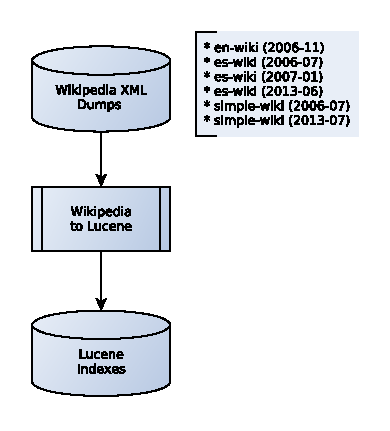
\includegraphics{graficos/LuceneIndexWriterWiki}
  \caption{Lucene Index Writer para dumps de Wikipedia}
  \label{fig:LuceneIndexWriterWiki}
\end{figure}


\subsection{Anotado de la pregunta}
\cerradaarg{Sin supervisar}
El módulo original de QA-sys de procesamiento de la pregunta espera preguntas en el formato Aquaint definido por Trec, al igual que el tipo de datos esperado sobre el corpus en el paso anterior. En el procesamiento lleva a cabo las tareas descriptas de modo general en \allref{subsec:impl-pos}, \allref{subsec:impl-ner} y \allref{subsec:qtype},  utiliza como librerías de procesamiento de lenguaje las el POS-Tagger, el NER-Tagger y el Question Classifier de la Universidad de Stanford, disponibles solo para inglés, descriptas en \allref{sec:stanford-both} y \allref{sec:stanford-qc} respectivamente.
En nuestra adaptación incorporamos los módulos de POS y NERC multilingües de freeling. Con respecto a la clasificación de preguntas, ya mencionamos que no existen clasificadores para español {\color{red} y tampoco para el portugués}. Frente a esta situación podríamos haber implementado clasificadores heurísticos basados en reglas escritas a mano como en el caso del sistema estructurado (\allref{sec:qp-mitic}). Aprovechando la disponibilidad de una traducción confiable al inglés de las preguntas en archivos de datos (debido a la activación de los ejercicios cross-lingual en-es y en-pt), decidimos utilizar el clasificador de Stanford sobre la traducción inglesa de la pregunta.
Las tablas \ref{table:x} y \ref{table:x} presentan la distribución de las 200 preguntas para español y para portugués según las cincos clases principales del esquema de Li \& Roth. Los niveles de confianza en la clasificación logradas oscilan entre tanto y tanto, dato dato dato.


\subsection{Generación de Respuestas}
\subsubsection{Baseline}
\falta
Como baseline de desarrollo y pruebas, adaptamos los algoritmos de Qanus. 
El procesamiento realizado por este módulo del paquete puede estructurarse así:
\begin{itemize}
  \item Filtrado de preguntas
  \item Generación de Queries
  \item Information Retrieval
  \item Extracción y rankeo de oraciones
  \item POS tagging de las mejores oraciones
  \item Heurísticas de AR basadas en el QC
\end{itemize}
En esta subsección vamos a describir esta implementación con detalle, mencionando los cambios más importantes que realizamos para adaptarla a la tarea elegida. En las siguientes comentaremos diferentes modificaciones y algoritmia agregada basada en la literatura. 

El proceso de qanus consiste DETALLE DE LA IMPLEMENTACION DE QUANUS.

Qanus solo trabaja sobre preguntas de tipo "FACTOID". Esto descarta "NO FACTOID" preguntas para español y "NO FACTOID" preguntas para portugués. Esta información depende de los experimentos y las comparaciones.

Para la generación de queries, el sistema baseline tiene 4 algoritmos diferentes según QType, es decir, según el resultado de Question Classifier. 
Los casos son los siguientes:
\textbf{Casos especificos para \sq{HUM:ind}} \\
Hay 3 casos especiales para 'HUM:ind', que se chequean contra regexs. En nuestra adaptación ml del sistema baseline, realizamos estos chequeos contra la traducción al inglés de la pregunta original, disponible en los xml de input. Hacer estadísticas con las preguntas. Descomentar y adaptar código. 

$HUM\_IND\_TYPE1\_IC$

$"[wW]ho/WP (is/VBZ|was/VBD)(([ A-Za-z0-9'\\-]+/NN)*([ A-Za-z0-9'\\-\\?]+/NN)+)") || a_QuestionTextPOS.matches("[wW]ho/WP (is/VBZ|was/VBD) the/DT (([ A-Za-z0-9'\\-]+/NN)*([ A-Za-z0-9'\\-\\?]+/NN)+)"$

$HUM\_IND\_TYPE1$

$"[wW]ho/WP (is/VBZ|was/VBD)(([ A-Za-z0-9'\\-]+/NN)+ of/IN(([ A-Za-z0-9'\\-]+/[A-Z]+)*([ A-Za-z0-9'\\-\\?]+/[A-Z]+)+))")|| a_QuestionTextPOS.matches("[wW]ho/WP (is/VBZ|was/VBD) the/DT (([ A-Za-z0-9'\\-]+/NN)+ of/IN(([ A-Za-z0-9'\\-]+/[A-Z]+)*([ A-Za-z0-9'\\-\\?]+/[A-Z]+)+))"$
			
$HUM\_IND\_TYPE2$

$"[wW]ho/WP( )([^w]+/VBD(([ A-Za-z0-9'\\-]+/[A-Z]+)*([ A-Za-z0-9'\\-\\?]+/[A-Z]+)+))"$

\textbf{Default: FormQuery} \\
El sistema original espera como parámetro, además de la pregunta propiamente dicha, un campo "target", aparentemente definido en la competencia TREC para la que está escrito. 
Utilizamos este valor esperado para completar con el "topic" del grupo de preguntas, lo cual no está permitido en las reglas originales de la competencia. 
El método default FormQuery genera una query que contiene, sin repetir, todas las palabras no-stopwords del campo target y todos los sustantivos, verbos y adjetivos de la pregunta completa según el pos tagger de stanford. 

A partir de la query generada, se hace un pedido al índice lucene. Los documentos son divididos en oraciones de manera indiscriminada, es decir: las oraciones no heredan posición de acuerdo al ranking de los documentos a los que pertenecían.

Las oraciones se evaluan mediante diferentes métricas contra la query generada. La fórmula de ponderación es la siguiente: \\
$l_DocScore += (0.9)*l_CoverageScore + (0.05)*l_FreqScore+ (0.05)*l_ProxScore;$

Siendo estas los descriptas en Anexo tal.

Finalmente, sobre las 40 oraciones mejor rankeadas aplica diferente heurísticas segun el QType.
Define heurísticas para los siguientes casos:
\begin{itemize}
  \item ABBR:exp
  \item ABBR:abb
	\item HUM:gr || ENTY:cremat
  \item HUM:
  \item NUM:period
  \item NUM:count
  \item NUM:
  \item ENTY:
  \item Else
\end{itemize}

\textbf{Adaptación inicial contra inglés}

Como las tareas cross-lingual y monolingual se cruzaban, estaban disponibles también en inglés las preguntas para nuestras tareas. 
Como paso de desarrollo, implementamos una solución sobre una wikipedia en inglés con las herramientas de procesamiento originales del baseline: StanfordNER y StanfordPOS. Lamentablemente, la tarea inglés-inglés no fue propuesta, por lo que no disponemos de las goldstandard answers como las que disponemos para español y portugués. De todos modos, realizamos experimentos sobre este sistema, utilizando la wikipedia en inglés de noviembre de 2006. En el apéndice correspondiente pueden encontrarse resultados sobre estos experimentos.

Ver \allref{chap:resultados-ingles-simple} para una tabla de los datos.

\textbf{Baseline multilingüe}

\subsubsection{Group Entity extraction}
\label{subsubsec:entidad-de-grupo}
\falta
Formas de extraer la entidad de grupo o tópico y de incorporarlo en la query.
\subsubsection{Query Generation}
\falta
Baseline de Qanus.
Resultados.
\subsubsection{Passage Extraction}
\falta
\subsubsection{Lasso Heuristics}
Métricas de medición: definición de documento relevante.
\subsubsection{Qanus baseline}
\falta
\subsubsection{Heuristic 1}
\falta
\subsubsection{Heuristic 2}
\falta
\subsubsection{Heuristic 3}
\falta
\subsubsection{Experimentación de Answer Retrieval}
\falta


\section{Evaluación}
\falta
\subsection{Evaluación y resultados de Clef}
\falta
Como en años anteriores, la respuesta correcta pudo estar copiada y pegada exactamente desde el documento, aún cuando sea gramaticamente incorrecta (por ejemplo: el caso de inflexión no coincide con el requerido por la pregunta). De todos modos, este año se les permitió a los sistemas usar generación de lenguaje natural para corregir inconsistencias morfosintácticas. (Por ejemplo, en alemán cambiar “dem Presidenten” por “der President” si la pregunta implica que la respuesta está en caso nominativo) y para introducir cambios gramáticos y léxicos (por ejemplo: Pregunta: ¿De qué nacionalidad es X? Respuesta: X es de Holanda => Respuesta Exacta: Holandés).


% \chapter{Implementación}
% \label{chap:implementacion}

% \section{Frameworks}

% \subsection{No funcionales}

% Para la implementación de nuestro sistema, originalmente, evaluamos la
% utilización de distintos frameworks disponibles. DeepQA, el producto
% de IBM, no es de código abierto, por lo que acerca de su
% implementación sólo sabemos lo que ventilaron en sus artículos
% técnicos. Just.ask, el sistema basado en web comparado contra
% OpenEphyra no está disponible en la web al momento de escribir este
% trabajo, mientras que OpenEphyra no funciona tal cual está dise\~nado
% originalmente (basado en web), sino que el autor sugiere unos pasos
% esotéricos para configurarlo para usar conocimiento local. Cabe
% destacar que esta falla en la funcionalidad está asociada a la que
% había encontrado [AUTOR DE PAPER EPHYRA1] en Aranea y está
% vinculado con una serie de medidas restrictivas tomadas por las
% compa\~nías de buscadores, que fueron cerrando sus accesos gratuitos
% para la comunidad de investigación bloqueando sus APIs y el acceso
% automático a sus UI. Las alternativas para el uso de buscadores,
% actualmente, se reducen a la configuración de una serie de proxies
% sobre los que rotar el acceso a la UI y así enga\~nar al detector de
% accesos automáticos -alternativa de legalidad cuestionable - o bien al 
% pago por una quota de queries por mes.
% OpenEphyra sobrevivió a Aranea porque sus responsables escribieron
% una interfaz para Bing cuando Google cerró sus puertas, mientras que
% los responsables de Aranea no lo hicieron. Finalmente, Bing también
% bloqueo el acceso automático gratuito. Notar que el mismo tipo de
% discontinuación ocurrió con el API de traducciones de Google. La
% empresa declara, explícitamente, que no está dispuesta a acceder a
% ninguna quota de acceso gratuito para la investigación académica y
% que todos sus servicios son pagos. 

% %Tanto de Aranea como de OpenEphyra podríamos llegar a tomar algunos de
% %sus componentes a la hora de construir nuestro sistema. Por el momento,
% %fueron simplemente dejados de lado.

% \bigskip

% \subsection{Qanus}

% Finalmente, un sistema que \textit{sí} estaba disponible y funcionando
% fue Qanus, que respetaba al pie de la letra su detalle técnico. Al comienzo
% del proyecto, contábamos con un corpus de datos en XML,
% lo cual coincidía, al menos en gran parte, con el input esperado de
% la implementación Qa-sys. A pesar de esto, la adaptación de los
% componentes no fue nada trivial y requirió un tiempo excesivo. En
% particular, existían dos opciones a la hora de construir un sistema
% sobre la arquitectura Qanus: dejar de lado la implementación Qa-sys e
% implementar todos los componentes de cero sobre la arquitectura, respetando las interfaces
% dadas por el framework, o adaptar el sistema funcionando para que
% trabaje sobre los nuevos datos y el nuevo entorno esperado. Frente a
% esta alternativa, se aparece claro que el framework en sí mismo no
% aporta demasiado, pues lo único que hace es atar la implementación
% final a una interfaz estructurada de tres procesos bastante sencillo.
% Además, existe un cierto grado de dependencia de la arquitectura
% hacia la implementación final, quizás no a nivel técnico, pero si
% en el modo en el que está definida la estructura. Por este motivo,
% encaramos una adaptación de Qa-sys a nuestro modelo de datos y a
% nuestros requerimientos, pero los resultados no fueron buenos en
% términos de resultados por tiempo invertido. El tiempo de aprendizaje
% del framework mismo y el tiempo requerido para adaptar las distintas
% componentes propias a las interfaces esperadas por Qanus es demasiado
% alto para la solución que brinda. Como recién mencionamos, en
% realidad, el proceso de pipeline de tres pasos no tiene tantas aristas,
% y adaptarse a un framework es mucho menos ameno que escribirlo. Este
% puede ser uno de los motivos por los cuales, como acertadamente
% se\~nalan los autores de Qanus, no existe ningún framework
% estandarizado dentro del ámbito de la investigación en QA.
% Después de la investigación inicial, podríamos concluir que
% está estandarizado, al menos a modo conceptual, la idea de que la
% resolución del problema se debe enfocar como un pipeline de al menos
% tres pasos que incluyen:
% \begin{itemize}
% \item el preprocesamiento de la base de conocimiento,
% \item el preprocesamiento de la pregunta,
% \item el retorno de la respuesta a partir de los resultados de los dos pasos anteriores. 
% \end{itemize}
% Como último comentario al respecto, el modelo de Qanus resultaba poco atractivo
%  a la hora de incorporar procesamiento en varios idiomas: el mejor approach
% utilizando esta arquitectura era implementar dos sistemas basados en
% Qanus paralelos y utilizar uno u otro de acuerdo con el resultado de
% una detección inicial. 

% \bigskip

% Si bien el modelo de Qanus fue, por los motivos recién expuestos,
% dejado de lado, debemos destacar una serie de puntos en los que fue
% útil.

% En primer lugar, uno de los objetivos de Qanus es facilitar el ingreso
% al área del QA de nuevos investigadores. Creemos que esto está
% logrado perfectamente: el código es muy sencillo y claro y lo mismo
% ocurre con la documentación, lo que hace de Qanus un proyecto muy
% útil desde una perspectiva pedagógica o educativa, más allá de
% que sea esta misma simpleza la que más adelante atente contra la
% usabilidad. El modelo de pipeline, que es el enfoque teórico usual al
% problema, y los distintos componentes y usos típicos de estos
% componentes en los distintos pasos del pipeline se realizan linealmente
% en la implementación de Qanus y Qa-sys. En particular, la similaridad
% entre la descripción del código de IBM (DeepQA y Watson) y el
% enfoque con el que Qanus ataca el mismo problema salta a la vista,
% considerando la diferencia de escalas. 

% En segundo lugar, en el plano de la investigación del estado de arte
% de los sistemas de QA disponibles creemos que el intento con Qanus
% redundó en un cierto escepticismo sobre la posibilidad de resolver
% nuestro problema utilizando herramientas disponibles de gran escala. La
% conclusión es análoga a la que tuvo el equipo de IBM al intentar
% usar OpenEphyra y PIQUANT: el tiempo de customización y adaptación
% de los framework a nuestro problema puntual es demasiado alto en
% comparación con el tiempo necesario para construir una nueva
% arquitectura que cumpla los mismos requisitos. 

% Por último, en un nivel técnico, Qanus nos resultó de utilidad para
% construir nuestro modelo final pues reutilizamos varios de los
% componentes de Qa-sys: En primer lugar, recuperamos el POS tagger, el
% NER tagger y el Question Classiffier (QC) de Stanford, que son las
% librerías principales con las que Qa-sys encara el procesamiento
% lingüístico de la pregunta y parte del proceso de generación de
% respuestas. Todas estas herramientas están disponibles en la web por
% otros medios, pero algunas -principalmente el QC- requieren un cierto
% tiempo de configuración inicial que los autores de Qanus ya habían
% resuelto. Es decir, reutilizamos, además de estos módulos externos,
% bastante de la configuración y las APIs de acceso a estos módulos
% escritos por los singapurenses. Estas herramientas funcionan bien
% sólo para inputs en inglés. Las adaptaciones que hicimos las
% veremos más abajo. Por otro lado, incorporamos casi sin
% modificaciones algunas métricas de distancia entre pasajes que Qa-sys
% usa en el momento de la generación de la respuesta como Scorers.
% Estos son las clases: \textbf{FeatureSearchTermCoverage},
% \textbf{FeatureSearchTermFrequency}, \textbf{FeatureSearchTermProximity},
% \textbf{FeatureSearchTermSpan}. Explicaremos esta métricas en breve, dentro de nuestro
% modelo, bajo en nombre de
% {\textquotedblleft}Comparadores{\textquotedblright}. Este código
% está escrito por los autores de Qanus (es decir, no es una librería externa utilizada por ellos).


% \bigskip

% \section{Arquitectura}

% \subsection{Motivación}

% En este dise\~no respetamos el modelo típico de pipeline de tres pasos que
% abunda en la literatura científica y, por lo demás, parece el
% indicado a la hora de encarar este tipo de problemas. Un momento no-técnico
% importante a destacar es la obtención de una base de datos en
% mongodb, resultado del trabajo del proyecto MITIC, la cual cambió
% sustancialmente el enfoque anterior, basado en XMLs. 
% A partir de estos datos, fue posible delinear un esquema de entidades formal que determinó
% qué se puede responder y qué no. Como vimos, la estrategia de QA
% cuando el tipo de datos es estructurado es radicamente distinta que la
% estrategia cuando los datos son no estructurados. Qanus, por su parte,
% está orientado a un tipo de datos no estructurados: buscar documentos
% rankeados en un índice de búsqueda y rastrear en ellos pasajes
% mediante distintos métodos. Cuando la base de conocimientos consta de
% un tipo de datos estructurado (esto es, de entidades, relaciones,
% atributos de entidades) es posible delimitar una ontología más
% rígida que permita concentrarse en la interpretación de la pregunta
% hacia un lenguaje formal. El arquetipo de este enfoque puede pensarse
% como la traducción de un lenguaje de consulta humano a un lenguaje de
% consulta formal, como por ejemplo, SQL: esta estrategia de QA puede
% entenderse \ como una interfaz inteligente a una base de datos. \ En
% eje principal en este acercamiento está en el análisis
% lingüístico de la pregunta a fin de mapearla a un dominio conocido
% y, por otro lado, no es necesario hacer análisis lingüístico
% sobre el corpus de datos.


% \subsection{Base de datos de dominio cerrado}
% \subsection{Ejercicios de dominio abierto}
% \bigskip





% \subsection{No Estructurado}

% El proceso de generación de respuestas para los ejercicios de la Clef es muy distinto del anterior y puede dividirse en tres pasos principales: obtención de documentos y pasajes, ranking de pasajes y generación de respuesta. En el primer paso se accede a los índices invertido (al corpus) buscando documentos relevantes. Este paso pertenece netamente al área information retrieval. Como mencionamos al comentar Watson (en particular, ver \allref{subsec:deep-qa}), es fundamental que el resultado de este paso sea lo suficientemente amplio como para contener la respuesta pero lo suficientemente acotado como para no sobrecargar el proceso posterior de análisis lingüístico sobre los pasajes. Los documentos rankeados se dividen en pasajes. En el segundo paso, tanto los documentos como los pasajes son contrastados con distintas métricas contra los datos de la pregunta generando distintos valores para estos features. Finalmente, con esta información se procede al tercer paso, que consiste en realizar diferentes filtrados sobre los pasajes en función del tipo de respuesta esperado y en distintas formas de recopilar evidencia a favor de un pasaje o una entidad (depende el caso) para finalmente seleccionar una respuesta (o decidir que no se encontró ninguna).

% \begin{figure}[H]
%   \centering
%     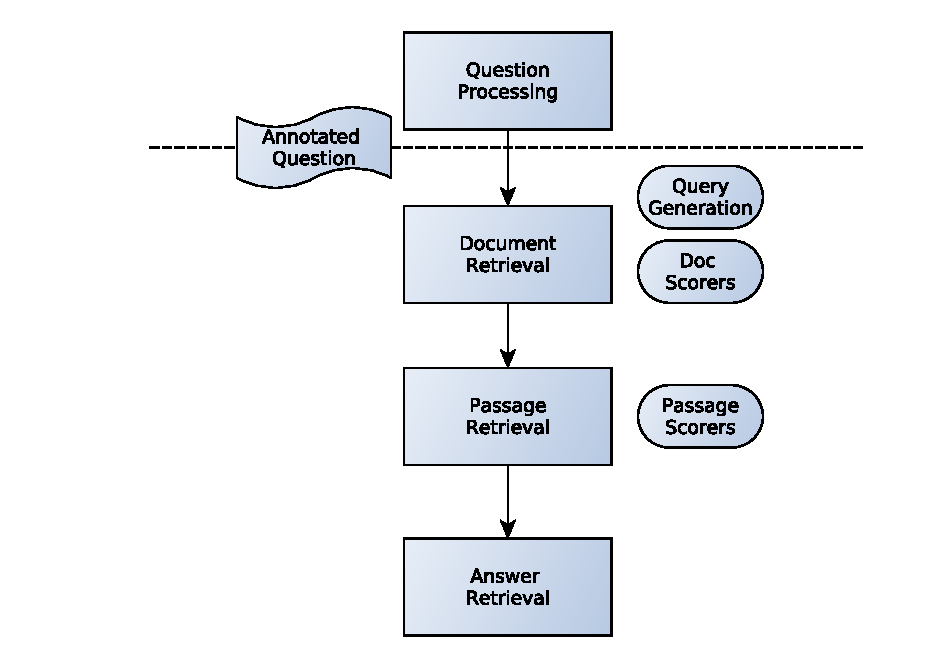
\includegraphics[scale=0.75]{graficos/AnswerRetrievalFlowWiki}
%   \caption{Flow para la Generación de Respuestas - No Estructurado}
%   \label{fig:AnswerRetrievalFlowWiki}
% \end{figure}

% \subsubsection{Documentos}
% \label{subsec:docs}
% En este punto, para una pregunta dada se dispone de la entidad del grupo de preguntas y de las distintas anotaciones hechas a la pregunta en el paso anterior (\allref{sec:qprocess}). Por su parte, los documentos en los índices invertidos poseen los campos $Id$, $Title$, y $Text$. El mecanismo de generación de queries tiene como objetivo priorizar en el ranking los documentos relacionados con el tema asociado al grupo de preguntas. Este paso es un problema de information retrieval puro: esto es, dado un pedido de información, retornar \textit{documentos relevantes}. El análisis semántico tiene peso en el paso posterior, a la hora de rankear pasajes. Por ejemplo, para el primer grupo de preguntas acerca de Harry Potter, solo se espera de este una lista de de documentos relacionados con ese mundo, en primer lugar. Por otro lado, es necesario que los principios de generación de queries no sean demasiado estrictos. Si en este punto quedan afuera muchas ocurrencias de una respuesta, entonces todo el resto del programa se ve afectado de manera irreparable. Es preferible generar documentos de más y luego filtrarlos mediante análisis lingüístico que ser demasiado estrictos y perder respuestas. 
% Para lograr esto, ponderamos los documentos en los que las entidades nombradas reconocidas lingüísticamente aparecen en el título, si se dispone de más de una entidad buscamos documentos que mencionen ambos, luego priorizamos los documentos que poseen estas entidades dentro del cuerpo y también consideramos la presencia de verbos en diferentes conjugaciones y de sustantivos que ocurren en la pregunta. Finalmente, agregamos una lista de documentos enviando la pregunta misma como una query.  

% Dado que finalmente se realizan queries simples (masivas), cabe preguntarse cual es la razón de la generación de queries y la ponderación de documentos. Esta razón es que en el proceso de ranking de pasajes y evaluación de respuesta se utilizan features basados en el score dado por lucene a los diferentes documentos. Si una mejor posición del documento contenedor del pasaje no implica que el pasaje sea correcto, si en cambio es un indicador de que dicho pasaje se encontró más cerca o más lejos del nucleo temático en el que se esperaba encontrarlo. 

% Una vez generada la lista de documentos rankeados según lucene, se procede a analizar algunos features en base a distintos scorers propios. A su vez, estos distintos valores se combinan en una evaluación general del documento, que será utilizada luego a la hora de generar una respuesta. Estas dimensiones buscan en el título y en el artículo diferente medidas sobre las entidades nombradas y sobre la pregunta completa. En concreto, se miden distancias a la entidad nombrada que identifica al grupo de preguntas (ver \allref{subsec:entidad-de-grupo}), las entidades nombradad en la pregunta misma, a la pregunta completa y la respuesta esperada data. Las medidas contra la respuesta esperada -dada por Clef- no pueden usarse para generar la respuesta, pero sí para evaluar la performance del sistema. En el siguiente cuadro se muestran las dimensiones que se consideran sobre los documentos. 

% \begin{center}
% \begin{tabular}{| l | l | l |}
% \hline
% Entidad & Campo & Comparador \\ \hline
% \multirow{6}{*}{Entidad de Grupo} & \multirow{3}{*}{Título} & Span \\ 
% & & Covr \\
% & & Freq \\ \cline{2-3}
% & \multirow{3}{*}{Texto} & Span \\ 
% & & Covr \\
% & & Freq \\ \hline
% \multirow{6}{*}{Entidades de Pregunta} & \multirow{3}{*}{Título} & Span \\ 
% & & Covr \\
% & & Freq \\ \cline{2-3}
% & \multirow{3}{*}{Texto} & Span \\ 
% & & Covr \\
% & & Freq \\ \hline
% \multirow{6}{*}{Todas las entidades} & \multirow{3}{*}{Título} & Span \\ 
% & & Covr \\
% & & Freq \\ \cline{2-3}
% & \multirow{3}{*}{Texto} & Span \\ 
% & & Covr \\
% & & Freq \\ \hline
% \multirow{6}{*}{Pregunta} & \multirow{3}{*}{Título} & Span \\ 
% & & Covr \\
% & & Freq \\ \cline{2-3}
% & \multirow{3}{*}{Texto} & Span \\ 
% & & Covr \\
% & & Freq \\ \hline
% \multirow{6}{*}{Respuesta} & \multirow{3}{*}{Título} & Span \\ 
% & & Covr \\
% & & Freq \\ \cline{2-3}
% & \multirow{3}{*}{Texto} & Span \\ 
% & & Covr \\
% & & Freq \\ \hline
% Score según índice & -- & -- \\ \hline
% \end{tabular}
% \end{center}

% Los comparadores señalados ($Freq$, $Covr$, y $Span$) se utilizan en distintos lugares de esta tesis y su funcionamiento es explicado en el apéndice \allref{sec:comparadores}. Notar que `Entidades de la pregunta' refiere tanto a aquellas reconocidas por el NER-tagger como a construcciones sustantivadas y que `Pregunta' no es la pregunta bruta sino la priorización de verbos conjugados, sustantivos, adjetivos y entidades. 

% El score general del documento es un cálculo ponderado de estas diferentes dimensiones. 

% Lucene permite especificar cuántos documentos queremos recuperar. Para evaluar la performance de este paso, utilizamos medida distintos scores en base a la respuesta dada por dada por la conferencia para el ejercicio. Es importante notar que dado que no utilizamos las imagenes de wikipedia de la primera sugerencia, es esperable que las respuesta no estén `tal cual'. 
% Evaluamos distintos mecanismos de generación de documentos, con distinta cantidad total, bajo distintas métricas. Para generar documentos, probamos la query trivial $ALL: pregunta$ (1), una un poco mejorada $ALL: entidad_de_grupo pregunta$ (2), secuencias concatenadas de queries tal como las describimos más arriba (3) y varios pedidos separados aplanados en un paso posterior (4). Para los cuatro métodos eliminamos los signos de puntuación. Para medir los resultados, utilizamos los comparadores de presencia exacta y diferentes grados de cobertura de términos (.8, .9 y 1). A su vez, evaluamos distintas imagenes de wikipedia para el español. Es total de preguntas del ejercicio, recordamos, es 200. Los resultados son los siguientes.

% \begin{center}
% \begin{tabular}{|l|l|l|l|l|l|l|}
% \hline
% Método & \# Docs & Wikipedia & Exacto & Covr 1 & Covr .9 & Covr . 8 \\ \hline

% \multirow{6}{*}{1 - Trivial} & 
% \multirow{3}{*}{100} & es - 2006 & 132 & 151 & 152 & 159 \\ 
%  &  & es - 2007 & 144 & 159 & 160 & 164 \\
%  &  & en - 2006 & x & x & x & x \\ \cline{2-7}
%  & \multirow{3}{*}{1000} & es - 2006 & 144 & 167 & 167 & 173 \\  
%  &  & es - 2007 & 159 & 177 & 177 & 180 \\
%  &  & en - 2006 & x & x & x & x \\ \hline

% \multirow{6}{*}{2 - Trivial'} & 
% \multirow{3}{*}{100} & es - 2006 & 138 & 156 & 157 & 164 \\ 
%  &  & es - 2007 & 151 & 167 & 168 & 171 \\
%  &  & en - 2006 & x & x & x & x \\ \cline{2-7}
%  & \multirow{3}{*}{1000} & es - 2006 & 147 & 168 & 168 & 174 \\ 
%  &  & es - 2007 & 163 & 178 & 178 & 181 \\
%  &  & en - 2006 & x & x & x & x \\ \hline
% hola & ey &wiki& 137 & 156 & 157 & 160  \\ \hline
% \multirow{6}{*}{3 - Inteligente} & 
% \multirow{3}{*}{100} & es - 2006 & 127 & 144 & 144 & 150 \\ 
%  &  & es - 2007 & 141 & 150 & 151 & 156 \\
%  &  & en - 2006 & x & x & x & x \\ \cline{2-7}

%  & \multirow{3}{*}{1000} & es - 2006 & 143 & 163 & 163 & 170 \\   
%  &  & es - 2007 & 158 & 175 & 175 & 179 \\
%  &  & en - 2006 & x & x & x & x \\ \hline

% \multirow{6}{*}{4 - Inteligente'} & 
% \multirow{3}{*}{100} & es - 2006 & 142 & 160 & 161 & 168 \\ 
%  &  & es - 2007 & 157 & 170 & 171 & 174  \\
%  &  & en - 2006 & x & x & x & x \\ \cline{2-7}


%  & \multirow{3}{*}{1000} & es - 2006 & 147 & 168 & 168 & 174 \\ 
%  &  & es - 2007 & x & 158 & x & x \\
%  &  & en - 2006 & x & x & x & x \\ \hline
 
% \end{tabular}
% \end{center}

% Conclusión de esto.

% \subsubsection{Pasajes}
% Este paso es análogo al anterior, pero con mayor detalle y granularidad. Cada documento generado en el paso anterior, con sus diferentes puntajes para 
% las dimensiones señaladas, se parten en pasajes u oraciones. Nuevamente, sobre estas oraciones realizamos diferentes mediciones y las combinamos generando
% un score final. En esta sección discutiremos las mediciones consideradas y los diferentes métodos de combinación de las mismas. Estos métodos de combinación generan distintos rankings de pasajes. Para evaluar estos rankings, nuevamente, utilizaremos la información disponible sobre las respuestas esperadas, buscando que la respuesta esperada se encuentre entre los $n$ pasajes mejor rankeados.
% En primer lugar, las distintos scorers implementados son los siguientes:

% \begin{center}
% \begin{tabular}{| l | l | l |}
% \hline
% Comparador & Qué & Dónde \\ \hline
% \multicolumn{3}{|c|}{Estadísticos} \\ \hline
% Freq & Pregunta & Pasaje \\ \hline
% Span & Pregunta & Pasaje \\ \hline
% Covr & Pregunta & Pasaje \\ \hline
% \#Tokens & -- & Pasaje \\ \hline
% \multicolumn{3}{|c|}{Basados en NLP} \\ \hline
% Presencia & Entidad de Grupo & Pasaje \\ \hline
% Presencia & Entidades de pregunta & Pasaje \\ \hline
% Presencia & Verbos de pregunta & Pasaje \\ \hline
% Presencia & Sustantivos de pregunta & Pasaje \\ \hline
% \multicolumn{3}{|c|}{Para evaluación} \\ \hline
% Freq & Respuesta & Pasaje \\ \hline
% Span & Respuesta & Pasaje \\ \hline
% Covr & Respuesta & Pasaje \\ \hline
% \end{tabular}
% \end{center}

% A estos Scorers se le suman los scores del documento asociado al pasaje (ver \allref{subsec:docs}). 
% Sobre estas dimensiones disponibles, intentamos las siguientes combinaciones de priorización:

% \begin{center}
% \begin{tabular}{|l|l|l|}
% \hline
% \#& Nombre & Fórmula \\ \hline
% 1& Simple & $2+2=4$ \\ \hline
% 2& Respuesta & $2+2=4$ \\ \hline
% 3& Compleja & $2+2=4$ \\ \hline
% \end{tabular}
% \end{center}

% Y consideramos la ocurrencia de respuestas, de la misma manera que en el apartado anterior (Match Exacto y tres medidas de covertura de tokens: 1, .9 y .8), 
% sobre los primeros $n$ pasajes, con $n$ = 1, 5, 10, 20, 50 y 100.

% \begin{center}
% \begin{tabular}{|l|l|l|l|l|l|}
% \hline
% Fórmula & \#Docs & Exacto & Covr 1 & Covr .9 & Covr . 8 \\ \hline
% \multirow{6}{*}{1} & 1 & x & x & x & x \\  \cline{2-6}
%  & 5 & x & x & x & x \\ \cline{2-6}
%  & 10 & x & x & x & x \\ \cline{2-6}
%  & 20 & x & x & x & x \\ \cline{2-6}
%  & 50 & x & x & x & x \\ \cline{2-6}
%  & 100 & x & x & x & x \\ \hline
% \end{tabular}
% \end{center}


% \subsubsection{Respuestas}





% \begin{figure}
%   \centering
%     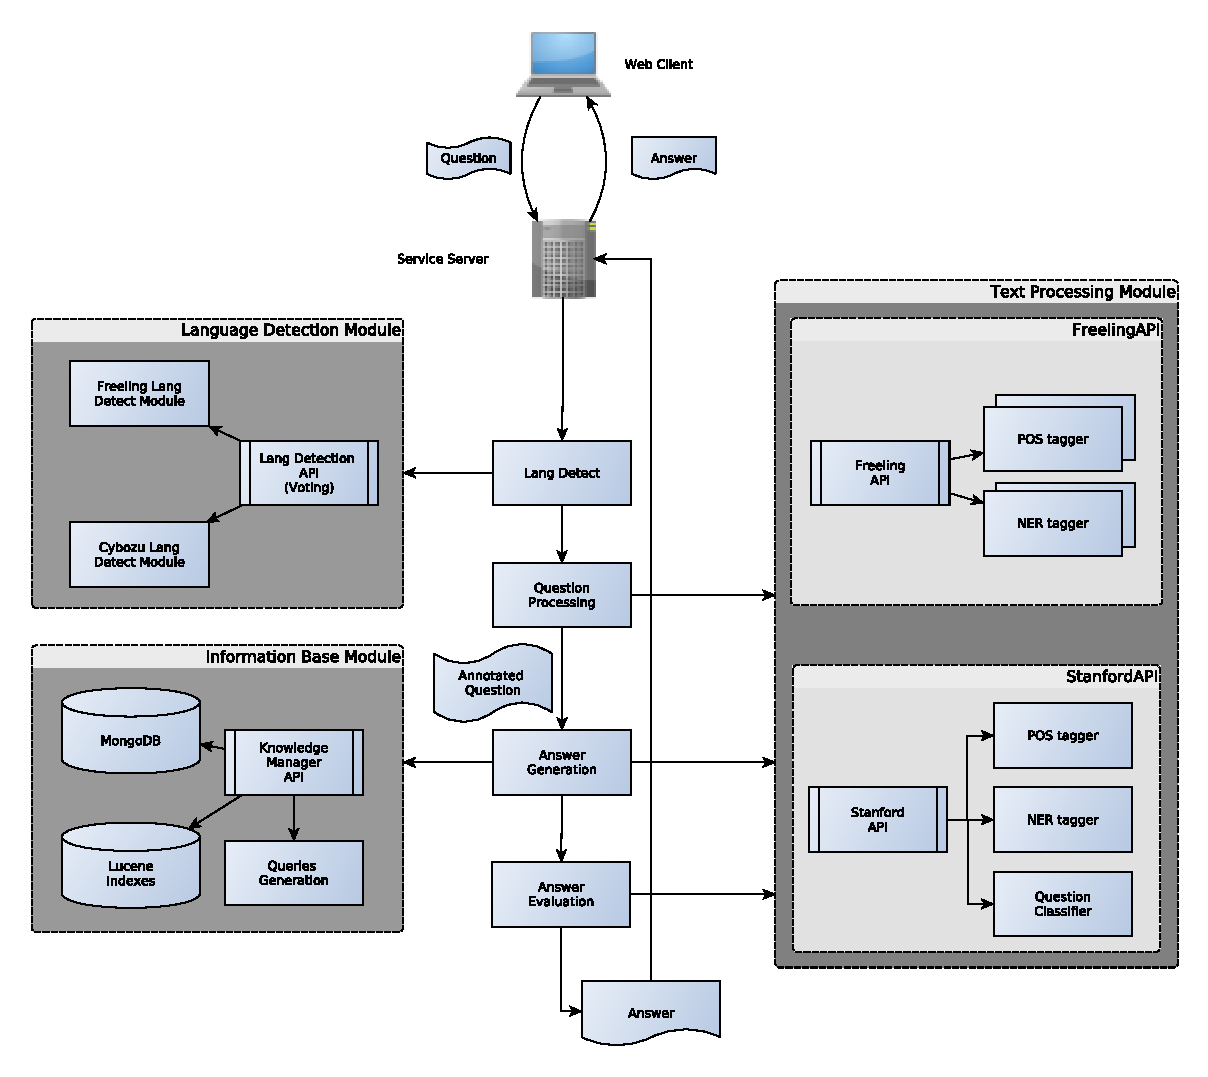
\includegraphics[scale=0.86]{graficos/Architecture}
%   \caption{Arquitectura}
%   \label{fig:Architecture}
% \end{figure}

% %\end{document}

\chapter{Conclusiones y trabajo futuro}


% \appendix
\nocite{*}

\begin{appendices}
  \appendix
\chapter{Herramientas}
\label{chap:herramientas}

\section{Stanford Question Classifier}
\label{sec:stanford-qc}
El Question Classifier de Stanford \cite{QC2} es un sistema de clasificación de preguntas basado en machine learning que utiliza la arquitectura de aprendizaje SNoW. Es un sistema jerárquico guiado por una semántica de dos niveles que permite la clasificación en categorías granulares. Según los tests de los autores, el proceso logra una efectividad del 90\% sobre 50 diferentes clases finales, utilizando features sintácticos y semánticos.

El clasificador dispone de una taxonomía de dos capas basada en los tipos de respuesta típicos de la TREC. Las clases superiores son seis: abreviatura, entidad, descripción, humano, lugar y numérico; divididas a su vez en 50 subclases más finas no solapadas (50 en total). La motivación de la existencia de clases superiores es doble: por un lado, ellas preservan compatibilidad y coherencia con las clases usadas en trabajos previos de clasificación de preguntas. Por otro, se esperaba obtener mejoras de performance aplicando dos fases de clasificación, pero esta intención no se corroboró en la experiencia

La tabla siguiente muestra la taxonomía de clasificación dividida en clases y subclases \footnote{Puede encontrarse en esta url: \url{http://cogcomp.cs.illinois.edu/Data/QA/QC/definition.html} y está explicada en \cite{QC2} y \cite{QC3}}


\begin{center}
\begin{longtable}{| l | l |}
\hline
Clase y subclase & Definición \\ \hline
ABBREVIATION &  abbreviation \\ \hline
  abb & abbreviation\\ \hline
  exp & expression abbreviated\\ \hline
ENTITY  & entities\\ \hline
  animal  & animals\\ \hline
  body & organs of body\\ \hline
  color & colors\\ \hline
  creative & inventions, books and other creative pieces\\ \hline
  currency & currency names\\ \hline
  dis.med. & diseases and medicine\\ \hline
  event & events\\ \hline
  food & food\\ \hline
  instrument & musical instrument\\ \hline
  lang & languages\\ \hline
  letter & letters like a-z\\ \hline
  other & other entities\\ \hline
  plant & plants\\ \hline
  product & products\\ \hline
  religion  & religions\\ \hline
  sport & sports\\ \hline
  substance & elements and substances\\ \hline
  symbol & symbols and signs\\ \hline
  technique & techniques and methods\\ \hline
  term  & equivalent terms\\ \hline
  vehicle & vehicles\\ \hline
  word & words with a special property\\ \hline
DESCRIPTION & description and abstract concepts\\ \hline
  definition & definition of sth.\\ \hline
  description & description of sth.\\ \hline
  manner & manner of an action\\ \hline
  reason & reasons\\ \hline
%\end{tabular}
%\begin{tabular}{| l | l |}
%\hline
HUMAN & human beings\\ \hline
  group & a group or organization of persons\\ \hline
  ind & an individual\\ \hline
  title & title of a person\\ \hline
  description & description of a person\\ \hline
LOCATION & locations\\ \hline
  city & cities\\ \hline
  country & countries\\ \hline
  mountain & mountains\\ \hline
  other & other locations\\ \hline
  state & states\\ \hline
NUMERIC & numeric values\\ \hline
  code  & postcodes or other codes\\ \hline
  count & number of sth.\\ \hline
  date  & dates\\ \hline
  distance &  linear measures\\ \hline
  money & prices\\ \hline
  order & ranks\\ \hline
  other & other numbers\\ \hline
  period  & the lasting time of sth.\\ \hline
  percent & fractions\\ \hline
  speed & speed\\ \hline
  temp & temperature\\ \hline
  size & size, area and volume\\ \hline
  weight & weight\\ \hline
\end{longtable}
\end{center}


Uno de los principales problemas que tuvieron los autores al enfrentarse a clases tan específicas fue la ambigüedad instrínseca de ciertas preguntas. Los siguientes ejemplos de este problema están tomados de \cite{QC2}:
\begin{itemize}
\item What is bipolar disorder? (¿Qué es el desorden bipolar?)
\item What do bats eat? (¿Qué comen los murciélagos?)
\end{itemize}
La primer pregunta puede pertenecer a la clase \textit{definición} o bien a la clase \textit{enfermedad / medicina} y la segunda a \textit{comida}, \textit{planta} o \textit{animal}. Para abordar este problema, el clasificador asigna diferentes clases ponderadas y no una única clase.

Los dos niveles de clasificación están implementados como dos clasificadores simples en secuencia, ambos utilizando el algoritmo Winnow de SNoW. El primero etiqueta la pregunta en función de las clases más generales y el segundo asigna las clases más finas (dentro de las suclases determinadas por la clase del primero).
El modelo para el algoritmo de aprendizaje representa las preguntas como listas de características (\textit{features}) tanto sintácticos como semánticos. Los features utilizando son, en total, más de 200.000, siendo casi todos combinaciones complejas de un set acotado de features simples basados en palabras, pos tags, chunks (componentes constitucionales de la oración), chunks principales (por ejemplo: componente nominal principal), entidades nombradas y palabras semánticamente relacionadas a ciertas clases. De estos seis tipos de features primitivos, tres son sintácticos (pos tags, chunks, chunks principales) mientras que otros son semánticos (named entities, palabras relacionadas).

El clasificador, al igual que el resto de las herramientas de nlp de Stanford, está implementado en java.


\section{Stanford POS \& NER Taggers}
\label{sec:stanford-pos}
\label{sec:stanford-both}
El POS tagger de Stanford es un algortimo basado en entropía máxima (\textit{maximum entropy}), implementado en java originalmente en \cite{POS2}, con algunos agregados y mejoras técnicas realizadas en \cite{POS1}. Al descargar el paquete, también está disponible uno más complejo con soporte para los idiomas árabe, chino y alemán. En este trabajo utilizamos el paquete sencillo, que consta de dos modelos entrenados para inglés, usando, como señalamos en \allref{subsec:pos} el tagset de Penn Treebank.


Por su parte, el NER tagger de Stanford, es una implementación general de

It comes with well-engineered feature extractors for Named Entity Recognition, and many options for defining feature extractors. Included with the download are good named entity recognizers for English, particularly for the 3 classes (PERSON, ORGANIZATION, LOCATION), and we also make available on this page various other models for different languages and circumstances, including models trained on just the CoNLL 2003 English training data. The distributional similarity features in some models improve performance but the models require considerably more memory.

Stanford NER is also known as CRFClassifier. The software provides a general implementation of (arbitrary order) linear chain Conditional Random Field (CRF) sequence models. That is, by training your own models, you can actually use this code to build sequence models for any task. (CRF models were pioneered by Lafferty, McCallum, and Pereira (2001); see Sutton and McCallum (2006) or Sutton and McCallum (2010) for more comprehensible introductions.)

The CRF code is by Jenny Finkel. The feature extractors are by Dan Klein, Christopher Manning, and Jenny Finkel. Much of the documentation and usability is due to Anna Rafferty. The CRF sequence models provided here do not precisely correspond to any published paper, but the correct paper to cite for the software is:

Jenny Rose Finkel, Trond Grenager, and Christopher Manning. 2005. Incorporating Non-local Information into Information Extraction Systems by Gibbs Sampling. Proceedings of the 43nd Annual Meeting of the Association for Computational Linguistics (ACL 2005), pp. 363-370. http://nlp.stanford.edu/~manning/papers/gibbscrf3.pdf
The software provided here is similar to the baseline local+Viterbi model in that paper, but adds new distributional similarity based features (in the -distSim classifiers). The big models were trained on a mixture of CoNLL, MUC-6, MUC-7 and ACE named entity corpora, and as a result the models are fairly robust across domains.
Named Entity Recognition Stanford Named Entity Recognizer (Finkel,
Grenager and Manning 2005)

Finkel, Jenny Rose, Trond Grenager, and Christopher Manning. "Incorporating
Non-local Information into Information Extraction Systems by Gibbs Sampling."
roceedings of the 43nd Annual Meeting of the Association for Computational
Linguistics. 2005.



\section{Freeling}
\label{sec:freeling}
\label{subsec:freeling-pos}
\label{subsec:freeling-mods}
Freeling es una librería de c\'odigo abierto que provee distintas herramientas de
procesamiento de lenguaje natural, desarrollada y mantenida por el Centre de Tecnologies
i Aplicacions del Llenguatge i la Parla (TALP) de la Universidad Politécnica de Catalu\~na (UPC).
Freeling está dise\~nado para ser usada como una librería externa y ofrece un API en distintos lenguajes
de programaci\'on. Su principal virtud es ser multilingüe, esto es, los diferentes analizadores que provee funcionan
para un conjunto bastante amplio de idiomas. La última versi\'on a la fecha (3.1) soporta los siguientes idiomas:

\begin{itemize}
\item Asturian (as)
\item Catalan (ca)
\item English (en)
\item French (fr)
\item Galician (gl)
\item Italian (it)
\item Portuguese (pt)
\item Russian (ru)
\item Slovene (sl)
\item Spanish (es)
\item Welsh (cy)
\end{itemize}

Cabe destacar que no todos los m\'odulos soportan todos los idiomas. Sin embargo, dado que el proyecto está radicado en Espa\~na,
los idiomas necesarios para los fines de nuestro trabajo (espa\~nol e inglés), soportan todos los m\'odulos disponibles
en la librería.
Freeling 3.1 ofrece los siguientes analizadores lingüisticos:

\begin{itemize}
\item Detecci\'on de idioma
\item Tokenizer
\item Sentence splitting,
\item Análisis morfol\'ogico
\item NER y NEC (Detecci\'on y Clasificaci\'on de Entidades Nombradas)
\item Reconocimiento de fechas, números, magnitudes físicas, monedas
\item Codificaci\'on fonética
\item POS tagging,
\item Shallow parsing
\item Dependency parsing
\item Wordnet-based sense annotation
\item Word Sense Disambiguation
\item Coreference resolution
\end{itemize}


El módulo de POS tagging de Freeling dispone de dos tagger. El primero, $hmm\_tagger$, es un algoritmo clásico que utiliza Hidden Markov Models (HMMs) con tri-gramas. La descripción del algoritmo de tagging basado en HMM se encuentra con detalle en  en \cite{POS0}. Por otro lado, el módulo incorpora un método llamado $relax\_tagger$ que permite la creación de un sistema híbrido que permite reglas escritas a mano y modelos estadísticos.

\section{Apache Lucene}
\label{sec:lucene}
Lucene es una librería de information retrieval, de c\'odigo abierto, escrita en Java y distribuida
bajo la licencia Apache Software License por la Apache Software Foundation. No está pensada para
usuarios finales sino para ser integrada dentro de proyectos informáticos, resolviendo
la parte de bajo nivel y brindando servicios a través de un API en diferentes lenguajes de programaci\'on.
Su core es un índice invertido como el que describimos anteriormente. La implementaci\'on de un sistema
que utiliza Lucene consta de dos pasos separados:
\begin{itemize}
\item La \textbf{creaci\'on} del índice, es por lo general un proceso offline en el cual
se incorporan distintas fuentes de informaci\'on al índice
\item La \textbf{búsqueda} de documentos en el índice creado en el paso anterior, a partir de una query
ingresada por el usuario final. Este proceso se incorpora dentro del flujo `online' del sistema.
El resultado de esta búsqueda es una lista de documentos rankeados con un cierto puntaje.
\end{itemize}

Es importante señalar que si bien el proceso de creaci\'on del índice suele estar desacoplado del resto
del sistema, las fuentes de informaci\'on no tiene por que ser `offline' en el sentido de ser documentos
en un disco local. De hecho, Nutch, otro proyecto de c\'odigo abierto de la Apache Software Foundation es
un motor de búsqueda web basado en Lucene que incorpora un crawler para indexar sitios web. Lucene soporta
cualquier fuente de informaci\'on que pueda convertirse en texto mediante algoritmia.
\newline
Los conceptos fundamentales de Lucene son: índice, documento, campo, término y query.
\begin{itemize}
\item Un índice contiene un conjunto de documentos
\item Un documento es un conjunto de campos
\item Un campo es el nombre de una secuencia de términos
\item Un término es un token (una palabra)
\item Una query es una lista de términos conectados con distintos operados l\'ogicos
\end{itemize}
  
\chapter{Placeholders}
\section{MyMemory}
MyMemory es la Memoria de Traducción más grande del mundo: 300 millones de segmentos a finales de 2009

Como las MT tradicionales, MyMemory almacena segmentos con sus traducciones, ofreciendo a los traductores correspondencias y concordancias. El proyecto se diferencia de las tecnologías tradicionales por sus ambiciosas dimensiones y por su arquitectura centralizada y basada en la colaboración colectiva. Todos pueden consultar MyMemory o hacer aportaciones a través de Internet; la calidad de las aportaciones será cuidadosamente ponderada.
MyMemory gives you quick access to a large number of translations originating from professional translators, LSPs, customers and multilingual web content. It uses a powerful matching algorithm to provide the best translations available for your source text. MyMemory currently contains 644.377.834 professionally translated segments.

Las memorias de traducción son almacenes compuestos de textos originales en una lengua alineados con su traducción en otras. Esta definición de memorias de traducción coincide literalmente con una de las definiciones más aceptadas de corpus lingüístico de tipo paralelo (Baker, 1995). Por esto se puede decir que las memorias de traducción son corpus paralelos.


Por el momento, no estamos utilizando ningún módulo de traducciones:
todo el enfoque multilingüe está dado por la detección del idioma
de la pregunta y la determinación de distintas herramientas de
análisis según qué idioma sea. Sin embargo, en un momento se
evaluó un enfoque distinto, basado en la traducción. Por ejemplo:
utilizar módulos de procesamiento sólo en inglés y
{\textquotedblleft}normalizar{\textquotedblright} los inputs en otros
idiomas (en principio, en espa\~nol), a este idioma interno, y luego lo
mismo con la generación de respuestas. A pesar de que no es el
enfoque actual, hubo una fase de investigación dentro del dominio de
la traducción, que resultó en un módulo de traducción basado en
MyMemoryAPI.

Intento con google translator y la privatización. ?`La falta de
software de traducción offline? El módulo de mymemory, robado de
algún lugar. El sistema de cobro. 

\section{Citas a Textos trascriptos pero no usados}
\begin{itemize}
\item QC: \cite{QC1}, \cite{QC2} y también \cite{QC3} (y \cite{QC-other})
\item Clef: \cite{GuidelineClef07} y \cite{OverviewClef07} 
\item POS: El manual \cite{POS0} y los dos de Stanford: \cite{POS1} y \cite{POS2}
\item LangDetect: \cite{nakatani2010langdetect}
\item NER: Survey \cite{NER1} y el NER de Stanford: \cite{NER2}
\item Watson: \cite{WATSON1} y \cite{WATSON2}
\item Qanus: \cite{QANUS1}
\item RE: Survey \cite{RE1}, for QA \cite{RE2} y reverb: \cite{RE3}
\item Ephyra: \cite{EPHYRA1}
\item Freeling: \cite{FREELING1} y \cite{FREELING2} (este no impreso)
\item Wordnet para web ir: \cite{WN1} (no leido)
\item Varios de QA: Yago \cite{YAGO-QA1}, sobre una teoria de QA como interfaz a DBs: \cite{QADB1}. Corpus: \cite{TRAIN-QA1}, qall-me: \cite{QALL-ME1}, practical QA: \cite{QAS1}, simple QA: \cite{QAS2} y Surface de Ravishandran: \cite{SURF1}. Introducción a QA: \cite{QA1} y \cite{QA2} y \cite{QA3}
\item Aranea: \cite{ARANEA1} (no leido)
\item Passage retrieval evaluation: \cite{PASSAGE1}
\item Evaluacion de las TREC8 (metrica de \cite{QA3} LASSO): \cite{TREC8}
\item QA survey: \cite{QA-survey}
\end{itemize}

\end{appendices}

%%%% BIBLIOGRAFIA
\backmatter
\bibliographystyle{apalike}
\cleardoublepage
\phantomsection
\addcontentsline{toc}{chapter}{Bibliografía}
\bibliography{tesis}


\end{document}
